% Options for packages loaded elsewhere
\PassOptionsToPackage{unicode}{hyperref}
\PassOptionsToPackage{hyphens}{url}
\PassOptionsToPackage{dvipsnames,svgnames,x11names}{xcolor}
%
\documentclass[
  11pt,
  a4paper,
]{book}
\title{De energietransitie doorgerekend}
\usepackage{etoolbox}
\makeatletter
\providecommand{\subtitle}[1]{% add subtitle to \maketitle
  \apptocmd{\@title}{\par {\large #1 \par}}{}{}
}
\makeatother
\subtitle{Welke samenstelling van zon, wind en kernenergie levert een haalbare mix op?}
\author{P. Maas}
\date{Proefversie 2.1, 2022-04-14}

\usepackage{amsmath,amssymb}
\usepackage{lmodern}
\usepackage{iftex}
\ifPDFTeX
  \usepackage[T1]{fontenc}
  \usepackage[utf8]{inputenc}
  \usepackage{textcomp} % provide euro and other symbols
\else % if luatex or xetex
  \usepackage{unicode-math}
  \defaultfontfeatures{Scale=MatchLowercase}
  \defaultfontfeatures[\rmfamily]{Ligatures=TeX,Scale=1}
\fi
% Use upquote if available, for straight quotes in verbatim environments
\IfFileExists{upquote.sty}{\usepackage{upquote}}{}
\IfFileExists{microtype.sty}{% use microtype if available
  \usepackage[]{microtype}
  \UseMicrotypeSet[protrusion]{basicmath} % disable protrusion for tt fonts
}{}
\usepackage{xcolor}
\IfFileExists{xurl.sty}{\usepackage{xurl}}{} % add URL line breaks if available
\IfFileExists{bookmark.sty}{\usepackage{bookmark}}{\usepackage{hyperref}}
\hypersetup{
  pdftitle={De energietransitie doorgerekend},
  pdfauthor={P. Maas},
  colorlinks=true,
  linkcolor={Maroon},
  filecolor={Maroon},
  citecolor={Blue},
  urlcolor={CornflowerBlue},
  pdfcreator={LaTeX via pandoc}}
\urlstyle{same} % disable monospaced font for URLs
\usepackage[margin=2cm]{geometry}
\usepackage{longtable,booktabs,array}
\usepackage{calc} % for calculating minipage widths
% Correct order of tables after \paragraph or \subparagraph
\usepackage{etoolbox}
\makeatletter
\patchcmd\longtable{\par}{\if@noskipsec\mbox{}\fi\par}{}{}
\makeatother
% Allow footnotes in longtable head/foot
\IfFileExists{footnotehyper.sty}{\usepackage{footnotehyper}}{\usepackage{footnote}}
\makesavenoteenv{longtable}
\usepackage{graphicx}
\makeatletter
\def\maxwidth{\ifdim\Gin@nat@width>\linewidth\linewidth\else\Gin@nat@width\fi}
\def\maxheight{\ifdim\Gin@nat@height>\textheight\textheight\else\Gin@nat@height\fi}
\makeatother
% Scale images if necessary, so that they will not overflow the page
% margins by default, and it is still possible to overwrite the defaults
% using explicit options in \includegraphics[width, height, ...]{}
\setkeys{Gin}{width=\maxwidth,height=\maxheight,keepaspectratio}
% Set default figure placement to htbp
\makeatletter
\def\fps@figure{htbp}
\makeatother
\setlength{\emergencystretch}{3em} % prevent overfull lines
\providecommand{\tightlist}{%
  \setlength{\itemsep}{0pt}\setlength{\parskip}{0pt}}
\setcounter{secnumdepth}{5}
\usepackage{float}
\usepackage[dutch]{babel}

\pagestyle{plain}
\setlength{\parindent}{24pt}
\setlength{\parskip}{2pt}

% zorg dat notes aan het eind van het hoofdstuk komen
% below is a trick that turns hyperlinks in text into footnotes: 
% \renewcommand{\href}[2]{#2\footnote{\url{#1}}}
% \usepackage{endnotes}
% \let\footnote=\endnote
% \renewcommand{\notesname}{Eindnoten}

% truuk om figuren tegen elkaar aan te krijgen
\newcommand{\squeezeup}{\vspace{-2.5mm}}

\usepackage{xcolor}
\definecolor{figachtergrond}{HTML}{F3F1ED}
\definecolor{boxachtergrond2}{HTML}{EEDBC3}
\definecolor{backbrown}{HTML}{F6EEDD}
\definecolor{headbrown}{HTML}{4C2B00}
\definecolor{backmoccasin}{HTML}{FFF0D7}
\definecolor{headmoccasin}{HTML}{4C2B00}
\definecolor{backblue}{HTML}{EEFAFF} 
\definecolor{headblue}{HTML}{013A4D}
\definecolor{financialtimes}{HTML}{FFEDEF}

\definecolor{onbenutsurplus}{HTML}{E8C4C4}
\definecolor{benutsurplus}{HTML}{C6E1BF}
\definecolor{hulpbron}{HTML}{56B4E9}
\definecolor{opslag}{HTML}{006300}
\definecolor{wind}{HTML}{00FF00}
\definecolor{zon}{HTML}{FFFF00}

\usepackage{tcolorbox}
\newtcolorbox{inhetkortbox}{
  colback=backbrown,
  colframe=white,
  coltext=headmoccasin,
  boxsep=5pt,
  arc=1pt}
\newtcolorbox{infobox}{
  colback=backblue,
  colframe=white,
  coltext=headblue,
  boxsep=5pt,
  arc=1pt}

\usepackage{colortbl}
\usepackage{booktabs}
\usepackage{longtable}
\usepackage{array}
\usepackage{multirow}
\usepackage{wrapfig}
\usepackage{float}
\usepackage{colortbl}
\usepackage{pdflscape}
\usepackage{tabu}
\usepackage{threeparttable}
\usepackage{threeparttablex}
\usepackage[normalem]{ulem}
\usepackage{makecell}
\usepackage{xcolor}
\ifLuaTeX
  \usepackage{selnolig}  % disable illegal ligatures
\fi
\usepackage[]{natbib}
\bibliographystyle{plainnat}

\begin{document}
\maketitle

\begin{titlepage}



\begin{center}

\bigskip

\bigskip

\bigskip

\bigskip

\bigskip

\bigskip

\bigskip

    \Large{Voor Knud} 
\end{center}

\end{titlepage}

{
\hypersetup{linkcolor=}
\setcounter{tocdepth}{4}
\tableofcontents
}
\hypertarget{aan-de-proeflezer}{%
\chapter*{Aan de proeflezer}\label{aan-de-proeflezer}}
\addcontentsline{toc}{chapter}{Aan de proeflezer}

Welkom! Dit project is een poging uit te vinden hoe de energietransitie er uit ziet, straks, als deze voltooid is. In principe zou er dan alleen nog CO\textsubscript{2}-vrij energie worden geproduceerd. Welke samenstelling van wind-, zon- en kernenergie levert een haalbare energiemix op? Wat werkt?

Dit project is onstaan uit een groepje geïnteresseerde mensen die zich afvroegen waar Nederland met de energietransitie op weg naar toe is. Een aantal daarvan hadden het fantastische boek van natuurkundeprof David MacKay -- \href{https://www.withouthotair.com/download.html}{\emph{Sustainable energy without the hot air}} -- gelezen en daaruit geleerd dat de meeste vormen van duurzame energie een lage energiedichtheid hebben. Tweederde van de groene energie werd in Nederland in 2019 bijvoorbeeld nog opgewekt door verbranding van gewassen (o.a. houtsnippers). Gewassen hebben een bedroevend lage energiedichtheid en het leek uitgesloten dat we daarmee straks \emph{net-zero} zouden bereiken. Waarom zetten we er dan op in?

Er lijkt niet echt een plan te zijn. Wat we niet konden ontdekken, in Nederland, maar ook in de rest van de rijke wereld, is met welke middelen we \emph{net-zero} daadwerkelijk zouden kunnen bereiken. Dat is eigenlijk vreemd, want de transitie vervangt fossiele energiebronnen met een hoge energiedichtheid door duurzame bronnen die een lage dichtheid hebben. Nederland is een klein land, en veel ruimte heeft al een bestemming. Zouden we het redden met windmolens? Met zon?

Het niet hebben van een plan kan grote gevolgen hebben. We mikken op `klimaatdoelen' kennelijk onder andere door in te zetten op het verbranden van houtsnippers, maar dat kan niet de eindoplossing zijn (Bedenk dat Europa in de middeleeuwen ontbost raakte omdat voor koken, verwarming en industrie hout de enige brandstof was. Hoe zouden we dat nu met een veel hoger verbruik wel voor elkaar moeten krijgen?). Het behalen van een kleine reductie brengt ons niet bij \emph{net-zero}. Zelfs het halen van een klimaatdoel brengt ons niet automatisch bij \emph{net-zero}. Is investering in techniek waarmee het einddoel niet wordt gehaald dan eigenlijk wel een slimme zet? Kan dat geld niet beter worden ingezet voor techniek die toekomst heeft, die ons op lange termijn tot \emph{net-zero} kan leiden?

Langzaam kwam de realisatie dat schaal in de energietransitie belangrijk is. Het is onvoldoende een bron te selecteren enkel omdat deze duurzaam is. Kan de bron ook voldoende worden opgeschaald om er \emph{net-zero} mee te bereiken? Het is belangrijk om na te denken over hoeveelheid, bijvoorbeeld hoeveel windmolens en zonnecellen er nodig zijn en waar je die neerzet.

Een tweede punt dat het groepje opviel is dat de twee opties waar nu voor wordt gekozen, zon en wind, lang niet altijd volop energie leveren. Wat doe je met windstilte? Opgevallen was dat vanaf eind september de zonnecellen op de boot niet meer voldoende waren om het verbruik te dekken en de accu's vol te krijgen, waar dat in de zomer nog probleemloos lukte. In de winter was men afhankelijk van de walstroom. Hoe werkt dat eigenlijk op het niveau van Nederland, als een heel land permanent energie nodig heeft?

Die vragen waren bij MacKay onderbelicht gebleven. Er wordt door hem kort gerekend aan de problematiek van uitval, maar niet voor de energiehuishouding van een heel land, voor een representatieve periode van vele jaren. Daarmee werd het huidige project eigenlijk geboren. Zou je dat voor Nederland kunnen schatten? Zou je kunnen schatten hoeveel extra molens je nodig zou hebben om uitval te voorkomen, of hoeveel accu's je nodig zou hebben om energie in te kunnen opslaan? Het bleek dat de KNMI daar geweldige data voor heeft: zoninstraling en windsnelheid per tijdsvakken van tien minuten, en dat over de afgelopen tientallen jaren. Dat leverde een berg met data waar een schatting mee gemaakt kon worden. Er werd programmacode geschreven om het uit te rekenen. De conclusies die daaruit konden worden getrokken hebben hun weerslag gevonden in deze tekst.

Helaas is Knud Boucher, de andere geestelijke vader van dit project, niet meer onder ons. Hij had een zeldzaam breed blikveld die werd gecombineerd met een kritische houding zonder daarbij de welwillendheid te verliezen. Hij wilde echt een oplossing. Als je de energietransitie zou willen laten slagen, hoe doe je dat dan zonder dat daarbij fysieke grenzen overschreden worden? Wat zou een verstandige aanpak zijn?

Onze inzet, die van Knud en die van mij, was om onderzoek te doen naar de mogelijkheden, zonder daarbij te kiezen voor een bepaalde uitvoering. Dat wordt graag overgelaten aan de democratische besluitvorming. Sommigen willen geen kernenergie, anderen vinden windmolens lelijk. Dat moet ieder voor zich weten, en wij met z'n allen op een of andere manier zien te besluiten. De tekst wil wat dat betreft neutraal zijn. Het gaat ons om de randvoorwaarden bij een bepaalde energiemix. Daarvoor is er gerekend aan verschillende inrichtingen van een energiemix. Wij hoopten te leren welke inrichtingen haalbaar zijn. Met haalbaar wordt bedoeld: het bereiken van \emph{net-zero}, zodanig dat Nederland zonder uitval van energie wordt voorzien. De insteek hier is om een eenvoudig rekenmodel te gebruiken om een schatting te maken van de schaal van de onderneming. Misschien geeft dat een indruk wat betere en wat minder goede oplossingen zijn.

Niet iedere duurzame energiebron wordt in het model meegenomen. Van de niet-continue energiebronnen leveren wind en zon het meeste op. Andere mogelijke bronnen zoals bijv. gewassen of aardwarmte werden minder zinvol geacht om mee te nemen wegens de lage opbrengst. De lezer wordt van harte aangeraden om MacKay er op na te slaan om zelf een indruk te krijgen van de potentie van verschillende energiebronnen. In tegenstelling tot dit stuk is MacKay vrij compleet. Hetzelfde geldt voor opslagmethoden, waar er drie van worden bekeken (accu's, spaarbekkens en waterstofopslag). Andere vormen zoals compressed air storage of ondergrondse opslagbekkens schalen slecht en worden minder zinvol geacht. Het kan natuurlijk zijn dat hierbij inschattingfouten zijn gemaakt en er een mooie vorm van opslag of energieopwekking ten onrechte genegeerd is. Hopelijk kan een toekomstige versie van de tekst daar dan op worden aangepast.

Natuurlijk ben je als (proef)lezer van harte uitgenodigd te reageren. Ik zou vooral willen dat de tekst neutraal en betrouwbaar is. \emph{Neutraal} in de zin dat er naar feiten wordt gekeken. Als de lezer ergens het gevoel krijgt dat er een keuze wordt opgedrongen, dan hoor ik het graag, want dat is niet de bedoeling. \emph{Betrouwbaar} in de zin dat de tekst en conclusies afleidbaar zijn. Bronverantwoording voor de gebrachte feiten moet betrouwbaar zijn. Naast MacKay wordt Wikipedia vaak gebruikt als bron. Voor factuele zaken wordt Wikipedia betrouwbaar genoeg geacht. Het is in ieder geval een openbare bron die makkelijk verder te toetsen is. Mochten er bepaalde feiten niet kloppen, of er een betere bronvermelding mogelijk zijn, dan kan een toekomstige versie daarop worden aangepast. Ik zou het geweldig vinden als de gebruikte feiten en bronnen in dit verhaal steeds beter geborgd zouden worden. De programmacode van de gebruikte berekeningen moet nog openbaar op internet breikbaar worden gemaakt, zodat ook deze gecontroleerd kan worden. Ik zou graag nog een onafhankelijk controleur over de schouders mee laten kijken of alle berekeningen kloppen. Zou je dat willen doen of ken je iemand, dan houd ik me zeer aanbevolen.

Tot slot: vind je het onderwerp belangrijk en de tekst iets toevoegen, geef het dan door. Voor wie de printversie heeft gekregen: er is ook een elektronische versie beschikbaar die zich makkelijker laat verspreiden.

\bigskip

\noindent
Dank voor het lezen!

\bigskip

\noindent
Pascal Maas,

\noindent
Januari 2022

\hypertarget{inleiding}{%
\chapter*{Inleiding}\label{inleiding}}
\addcontentsline{toc}{chapter}{Inleiding}

Peinzend werd er naar de molen opgekeken. Het ding is serieus groot. Op `t moment stond i stil. Er staat nauwelijks wind, genoeg om de boot voort te doen kruipen, maar onvoldoende om de molen te laten draaien. 'Als we straks nou veel van die molens hebben, voor onze energievoorziening, wat doen we dan op dit soort momenten?'

Een goede vraag. Zeilers willen graag windkracht vier, maar weten ook dat die er lang niet altijd staat. In het bijzonder niet in het weekend dat zij nu juist wilden gaan zeilen. Voor een land dat dag in, dag uit energie gebruikt, vormt uitval een nadeel.

Fossiele brandstoffen kunnen worden verbrand wanneer het uitkomt. De vraag naar energie kan altijd meteen worden beantwoord. Het feit dat wind en zon zelf bepalen wanneer zij produceren, schept een geheel nieuwe problematiek.

Wie met het autotootje, of, voor de dapperen onder ons, met de fiets, van het oude land het nieuwe inrijdt, ziet windmolens van horizon tot horizon. De Flevopolder telt ondertussen aardig wat windmolens, en ook in en langs het IJsselmeer is men druk aan het plaatsen.

Zon en wind zijn energiebronnen met een lage energiedichtheid in vergelijk met wat we nu zijn gewend van fossiele brandstoffen. We zullen meer moeite moeten doen, meer middelen moeten inzetten om hetzelfde niveau te behouden.

Hoe groot zijn deze problemen eigenlijk? Hoe ziet een voltooide energietransitie er eigenlijk uit?

Probeer de volgende vragen eens te beantwoorden. Wees niet bang om een gokje te doen. Hoeveel oppervlak van Nederland is er nodig om aan ons energiegebruik te voldoen met behulp van de wind? Hoeveel dagen per jaar waait het onvoldoende om in onze behoefte te voorzien? Hebben we in de winter iets aan zonne-energie? Is een combinatie van wind- en zonne-energie in staat om Nederland continu van energie te voorzien? Is het bijplaatsen van enkele kerncentrales afdoende om wind- en zonarme perioden door te komen?

Het is verbazingwekkend moeilijk om daar als geïnteresseerde burger een goed beeld van te krijgen. Informatie blijft vaak steken in details. Dat maakt het lastig een inschatting te maken met welke middelen de transitie het beste voltooid kan worden. Toch is het absoluut van belang daar een beeld van te krijgen. Als onze huidige ideeën en oplossingen niet zouden blijken te werken op de schaal die uiteindelijk nodig is, dan is er veel tijd en moeite verloren gegaan. Het is nuttig te proberen een beeld te krijgen van de grootte van de onderneming en de middelen die daarbij moeten worden ingezet.

Dat is wat dit project poogt te doen.

Het doel is om verschillende mogelijke inrichtingen van een energiemix door te rekenen om een idee te krijgen van de gevolgen de gekozen oplossing. Welke `mix' levert een haalbare oplossing op? De bedoeling is niet om een conclusie te souffleren. Het doel is uit te vinden hoe het zit, hoe het werkt. Puzzel gerust mee. Overtuig jezelf, in plaats van je te laten overtuigen. Dit project is onstaan uit een groepje mensen die chocolade wilde kunnen maken uit de constante stroom van media-artikelen en onderzoeken. Die wilden begrijpen hoe een energietransitie werkt, misschien wel net zoals jijzelf.

Een aantal uitgangspunten zijn belangrijk in de aanpak die hier wordt gehanteerd.

\emph{De interesse gaat uit naar een voltooide energietransitie}. De manier waarop er invulling wordt gegeven aan de huidige energietransitie, is door in te zetten op het behalen van klimaatdoelen. De middelen waarmee een klimaatdoel wordt bereikt zijn echter niet noodzakelijkerwijs de middelen waarmee ook \emph{net zero} behaald kan worden. Het kan zelfs averechts werken als de oplossingen waarvoor wordt gekozen inadequaat zijn om de transitie te volbrengen. Nadenken over een voltooide energietransitie dwingt tot nadenken over schaal. Ideeën die werken op kleine schaal doen dat niet noodzakelijkerwijs ook op grote schaal.

\emph{De berekeningen moeten gebonden zijn aan ons totale energieverbruik}. De productie van hernieuwbare bronnen wordt vaak afgezet tegen het elektriciteitgebruik van huishoudens. Elektriciteit vormt echter maar een beperkt gedeelte van het energiegebruik van een huishouden en huishoudens zijn maar een beperkt gedeelte van de economie. De berekeningen zullen uitgaan van het totale energieverbuik in Nederland: huishoudens, industrie, vervoer, alles.

\emph{De energievoorziening moet gewaarborgd blijven}. Het uitgangspunt is dat Nederland niet zonder energie mag komen te zitten. Dat betekent dat als er variabele energiebronnen worden gebruikt (zon en wind) de fluctuaties daarvan zullen moeten worden opgevangen door een alternatief.

\emph{De boekhouding moet kloppen}. Niets is makkelijker dan ons er van af te maken door eenvoudigweg alle energie uit het buitenland te betrekken. Het buitenland moet dat gewoon groen doen en we zijn collectief in één keer van ons schuldgevoel af. Knaagt er toch iets? Uiteindelijk is \emph{net zero} een mondiaal probleem. Hier wordt het benaderd door alleen naar Nederland te kijken. De productie van energie moet daarbij kunnen worden verantwoord. Een model dat energie importeert van elders, is lek. Waait het wel bij de buren? Hebben zij wel de energiecentrales neergezet die wij kennelijk niet bereid zijn te betalen?

De berekeningen richten zich in eerste instantie op fysieke haalbaarheid. Dat wil niet zeggen dat economie niet belangrijk is. Integendeel. De energietransitie is een massieve onderneming in vergelijk waarbij de Deltawerken kinderspel zijn. Ineffectieve keuzes kunnen duur uitpakken. Kosten zijn echter moeilijk te schatten. Het is afhankelijk van de ervaring die men met een proces heeft, de te produceren aantallen, van regelgeving. Al deze zaken veranderen in de loop van tijd. Wat misschien beter is dan kosten inschatten, is te proberen de fysieke gevolgen van een bepaalde keuze te achterhalen. Hoeveel windmolens zijn er nodig? Hoeveel energiecentrales? Het geeft een beeld van de complexiteit van de oplossing. Meer infrastructuur kost meer moeite om te realiseren. Een complexere oplossing is waarschijnlijk ook duurder.

\hypertarget{verbruik}{%
\chapter{Verbruik}\label{verbruik}}

\noindent Als de energietransitie eenmaal voltooid is, wordt alle energie in Nederland hernieuwbaar opgewekt. Alle fossiele brandstoffen zijn dan vervangen. Hoe gaat die toekomst eruit zien? Hoeveel windmolens, zonnecellen of kerncentrales zijn daarvoor nodig? Dat antwoord is afhankelijk van de hoeveelheid energie die Nederland gebruikt.

\hypertarget{bronnen}{%
\section{Bronnen}\label{bronnen}}

Het energieverbruik van Nederland wordt door het Centraal Bureau voor Statistiek (CBS) bijgehouden. In 2019, het jaar dat in deze tekst wordt gebruikt, was het totale energieverbruik 3047 petajoule (\href{https://opendata.cbs.nl/statline/\#/CBS/nl/dataset/83140NED/table?dl=38AA0}{Bron: CBS Energiebalans}). Figuur 1.1 neemt de data van het CBS als basis om een overzicht te krijgen van het totale verbruik. De figuur telt op tot 100\%.

\begin{figure}[!b]

{\centering 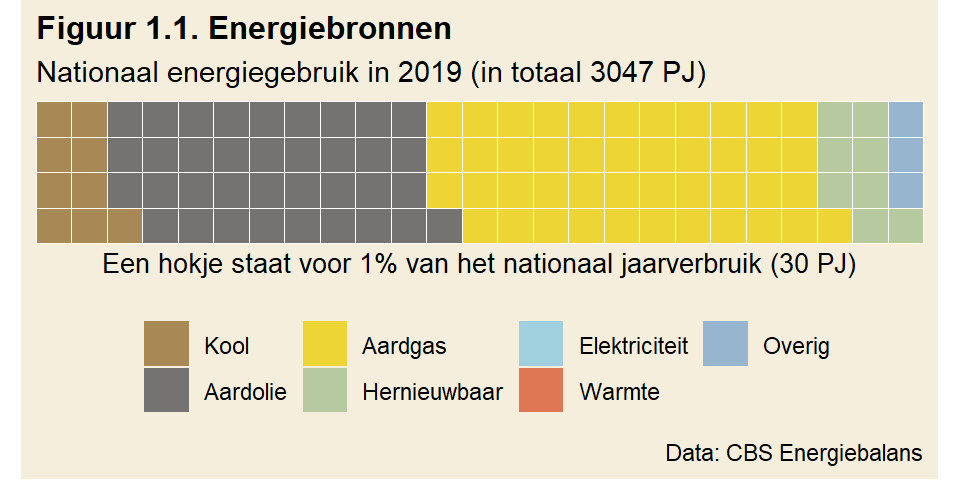
\includegraphics{02-Verbruik_files/figure-latex/figuur1_1-1} 

}

\end{figure}

Wat meteen opvalt is dat fossiele grondstoffen het overgrote deel van het energieverbruik uitmaken. Nederland draait dus, nog steeds, op aardgas, aardolie en kool. In totaal nemen deze fossiele bronnen 89\% van ons energieverbruik voor hun rekening.

Hoe zit het met hernieuwbare energie? In 2019 werd afgerond 8\% (figuur 1.1) van onze energie duurzaam opgewekt. Figuur 1.2 toont hoeveel er door iedere hernieuwbare bron apart werd geproduceerd. Ter vergelijk is ook kernenergie, als CO\textsubscript{2}-vrije bron, hieraan toegevoegd. Let op bij het tellen: de schaal is nu anders. Een vierkant staat nu voor een tiende procent van het nationaal energieverbruik.

Uit figuur 1.2 blijkt dat ruim een procent van ons energieverbruik wordt opgewekt door windenergie. Zonne-energie telt mee voor minder dan een procent en biomassa is goed voor ruim vijf procent. Wie kernenergie wil meerekenen, kan er nog een procent bij optellen.

Het grootste deel van de hernieuwbaar opgewekte energie komt dus voort uit \href{https://longreads.cbs.nl/hernieuwbare-energie-in-nederland-2019/biomassa/}{biomassa}. Biomassa bestaat onder andere uit hout- en afvalverbranding, en biotransportbrandstoffen die verplicht in benzine wordt ingemengd. Biomassa komt in oorsprong voort uit gewasgroei. De energiedichtheid van gewassen is laag in vergelijk met bijvoorbeeld de opbrengst van zonne- en windenergie (Zie \href{https://www.withouthotair.com/download.html}{MacKay}, p43, figuur 6.11). Op onze breedte kan zonne-energie 20 W/m\textsuperscript{2} leveren. Vergelijk dat met gewassen: MacKay gaat uit van 0,5 W/m\textsuperscript{2} voor `energy crops', o.a. hout. Biomassa concurreert rechtstreeks met landbouw of natuurgebied. In combinatie met de lage opbrengst per vierkante meter is het geen ideale vorm van brandstof.

\begin{figure}[!t]

{\centering 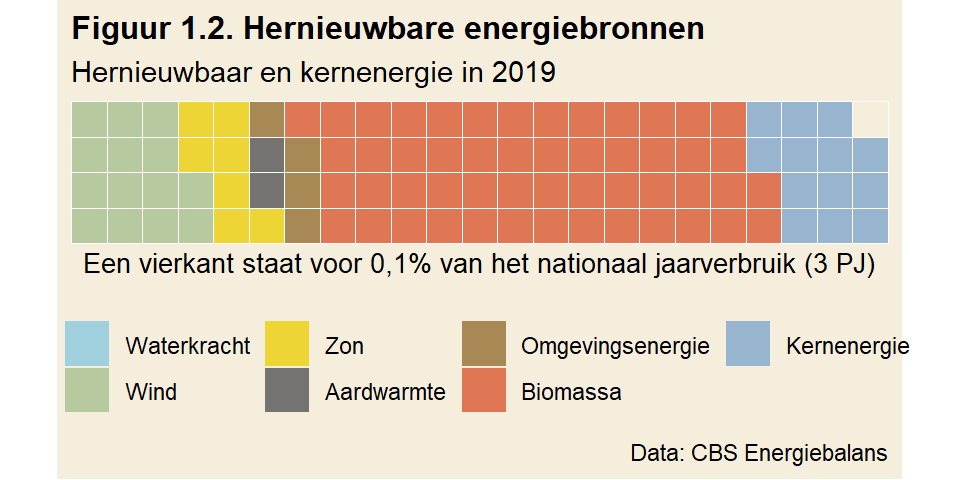
\includegraphics{02-Verbruik_files/figure-latex/unnamed-chunk-1-1} 

}

\end{figure}

Met kernenergie meegerekend als CO\textsubscript{2}-vrije bron, is uiteindelijk 9\% van het nationale energieverbruik CO\textsubscript{2}-vrij. Wil Nederland straks al zijn energie groen opwekken, dan is er dus nog een weg te gaan.

\hypertarget{omzettingen}{%
\section{Omzettingen}\label{omzettingen}}

De energiebronnen zoals opgesomd in figuur 1.1 worden door het CBS geclassificeerd als `aanbod'. Deze bronnen worden verder verwerkt. Een deel ervan wordt niet rechtstreeks gebruikt door afnemers, maar eerst omgezet in andere vormen van energie. Aardgas en kolen worden bijvoorbeeld deels omgezet in elektriciteit. Het resultaat van de omzetting wordt in Figuur 1.3 inzichtelijk gemaakt.

\begin{figure}[b]

{\centering \includegraphics{02-Verbruik_files/figure-latex/unnamed-chunk-2-1} 

}

\end{figure}

Elektriciteit maakt na omzetting 14\% uit van ons energieverbruik. Deels wordt dat al groen opgewekt, en deels vertegenwoordigt dat indirect gebruik van fossiele brandstoffen. Daarnaast is er direct verbruik door afnemers: voor 36\% van het totale energieverbruik wordt aardolie gebruikt en voor 25\% aardgas.

De gegevens in de energiebalans maken de omzettingen helaas niet expliciet. Er is niet af te leiden hoe bijvoorbeeld de 8\% hernieuwbare energie uit figuur 1.1 wordt omgezet. In figuur 1.3 resteert slechts 2\% `hernieuwbaar'. De overige 6\% is omgezet in andere vormen van energie, bijvoorbeeld elektriciteit.

\hypertarget{afnemers}{%
\section{Afnemers}\label{afnemers}}

Door wie worden al deze verschillende energievormen verbruikt? Het CBS houdt dat in de energiebalans voor iedere sector bij. Het wordt samengevat in figuur 1.4. Hierbij wordt de naamgeving van het CBS gevolgd, waarbij nadruk is gelegd op de grote verbruikers. Er kan weer geteld worden in de figuur: ieder vierkant staat voor een procent van ons nationaal jaarverbruik. De oplettende lezer merkt op dat de figuur optelt tot 84\%, dat komt omdat omzettingsverliezen niet meer meetellen.

Figuur 1.4 geeft een beeld door wie de verschillende energiebronnen worden verbruikt. Ons vervoer draait op aardolie en is goed voor 15\% van ons energieverbruik. Veel aardolie en ook wat aardgas gaan in het maken van producten (niet-energetisch gebruik, 17\%). Een fors deel van de bronnen wordt dus gebruikt om producten te maken. Denk bijvoorbeeld aan alles wat van plastic gemaakt wordt, maar er zijn natuurlijk vele andere voorbeelden. Huishoudens (categorie `Woningen') verbruiken 13\% van onze energie. Dat is voornamelijk aardgas, gebruikt voor verwarming. Dat zijn zo'n beetje de grote verbruikers.

\begin{figure}[b]

{\centering \includegraphics{02-Verbruik_files/figure-latex/unnamed-chunk-3-1} 

}

\end{figure}

\hypertarget{verbruik-1}{%
\section{Verbruik}\label{verbruik-1}}

Met welk energieverbruik moet men rekenen? Hoe groot was het energieverbruik van Nederland in 2019?

De energiebalans van het CBS somt energiedragers op, hoeveel van de drager gebruikt wordt en waarvoor. Een deel van de energiedragers wordt gevormd door grondstoffen, zoals aardolie of aardgas. Een ander deel van deze grondstoffen wordt \emph{niet} gebruikt voor de opwekking van energie, het zogenaamde `niet-energetisch gebruik'. Deze grondstoffen worden voornamelijk gebruikt voor producten. Trekt men dat af van het totaal, dan gebruikte Nederland in 2019 voor 2551 petajoule aan bronnen puur voor de opwekking van energie.

Hoeveel is dat, 2551 petajoule? Volgens het CBS (zie toelichting op de energiebalans): Petajoule (PJ) is een eenheid voor energie. Dit is 1 000 000 000 000 000 joule (een 1 met 15 nullen). Eén PJ komt overeen met 31,6 miljoen kubieke meter aardgas of 278 miljoen kilowattuur elektriciteit.

Hernieuwbare bronnen leveren vaak elektriciteit. Het is dus praktisch om het nationaal verbruik uit te drukken in een eenheid die veel wordt gebruikt bij elektriciteitsproductie. De terawattuur past daarbij het best als het gaat om het energieverbruik van een heel land (tera staat voor een 1 met 12 nullen). Omgerekend verbruikte Nederland in 2019 in totaal 706 TWh aan energie. Wie 706 TWh in een energieopslag heeft zitten, kan Nederland een jaar van energie voorzien. Gesteld dat de nationale energievraag constant is, verbruikt Nederland continu zo'n 81 GW aan energie (706 TWh / (365d * 24h) = 0,081 TW = 81 GW). Energiecentrales met een gezamenlijk vermogen van 81 GW kunnen Nederland permanent van energie voorzien.

\hypertarget{transitie}{%
\section{Transitie}\label{transitie}}

Wat worden de energiedragers van de toekomst? Daar lijken twee kandidaten voor te zijn: elektriciteit en waterstof, gemaakt van elektriciteit. De energietransitie is in die zin een transitie van fossiele brandstoffen naar elektriciteit. Processen die nu fossiele brandstoffen gebruiken, moeten omschakelen naar elektriciteit. De vraag is of dat in alle gevallen kan en de beste oplossing is.

Aangezien elektriciteit de energiebron van de toekomst is, ligt het voor de hand zoveel mogelijk processen te elektrificeren. Waterstof moet eerst geproduceerd worden, een proces dat op zichzelf energie kost. Elektriciteit gebruiken is dus in beginsel efficiënter. Daarnaast maakt elektrificatie in sommige gevallen het proces er efficiënter op. Dat zou meteen een besparing op het energieverbruik opleveren.

Persoonlijk vervoer is een goede kandidaat voor elektrificatie. Als het zou lukken ieder voertuig elektrisch te laten rijden, zou dat een besparing van 80\% op ten opzichte van de verbrandingsmotor kunnen opleveren (\href{https://www.withouthotair.com/download.html}{MacKay, p127}). Dat is meteen een aanzienlijke besparing ten opzichte van het totaal, want vervoer gebruikt 15\% van onze energie (figuur 1.4). Dit zou dus een besparing van 12\% op ons totale energieverbruik opleveren. Tenminste, als al het verkeer ge-elektrificeerd kan worden, maar dat lijkt met vrachtverkeeer niet het geval.

Een andere categorie waar winst valt te behalen, is `Woningen'. Het grootste verbruik hier is aardgas (9\%, zie figuur 1.4). Dat wordt voornamelijk gebruikt voor het verwarmen van huizen. Het kiezen voor een andere manier van verwarming, namelijk via warmtepompen, levert ook een besparing op. Een warmtepomp (een omgekeerde ijskast) kan een efficiëntie halen van 400\% of meer. Dat klinkt gek, maar een warmtepomp kan voor 1 kWh aan stroom 4 kWh aan warmte de kamer in krijgen (\href{https://www.withouthotair.com/download.html}{MacKay, p147}). Aangenomen dat verwarming via gas 100\% efficiënt is (wat niet gehaald wordt), kan hier (maximaal) een besparing van 75\% behaald worden. Dat zou betekenen dat hier een dikke 6\% besparing ten opzichte van het totale verbruik valt te behalen.

Zo bezien valt er dus best wat te besparen door efficiëntieverbeteringen, zonder dat daarbij aan comfort wordt verloren. Er zijn echter nog andere verbruikers te vinden in figuur 1.4: Chemie (5\% fossiel), Diensten (4\%), (overige) Nijverheid (4\%), de Energiesector (4\%) en Landbouw (2\%). Hoeveel van deze sectoren uiteindelijk ge-elektrificeerd kunnen worden is hier niet verder uitgezocht. Sommige zaken die niet ge-elektrificeerd kunnen worden, of waar het op z'n minst inefficiënt is, zijn industriële processen waarbij hoge temperatuur nodig is, vrachtvervoer, luchtvaart en openbaar vervoer (zie bijv. \href{https://energypost.eu/which-sectors-need-hydrogen-which-dont-transport-heating-electricity-storage-industry/}{hier}). Voor deze zaken ziet men waterstof als oplossing.

`Producten' (niet-energetisch gebruik, 17\% fossiel) is in dit plaatje een beetje een buitenbeentje. Afhankelijk van hoe hier tegenaan wordt gekeken, moet dit brongebruik ook vergroend worden of kan het juist buiten beschouwing worden gelaten. Vanuit de optiek dat alle fossiele brandstoffen vervangen moeten worden, omdat deze ooit uitgeput raken, zal ook dit fossiel gebruik moeten worden vervangen en dus worden meegeteld in de energierekening. Deze vervanging gaat waarschijnlijk juist meer energie vergen dan nu het geval is. De koolwaterstoffen die er nu voor worden gebruikt zijn in feite al `op voorraad', maar in de toekomst zullen deze moeten worden geproduceerd. Dat kost ongetwijfeld energie.

Een ander gezichtspunt is dat, aangezien productgebruik geen CO\textsubscript{2} uitstoot en de voorraad voorlopig niet uitgeput zal raken, dit kan worden weggestreept en aan toekomstige generaties kan worden overgelaten. Beide zienswijzen hebben hun merites. De berekeningen zullen uitgaan van alleen het energetisch gebruik.

Wat verder opvalt is het aandeel omzettingsverliezen (figuur 1.3), dat 16\% uitmaakt. Als deze verliezen bij verdere elektrificatie van de maatschappij voorkoombaar zouden zijn, dan levert dat in feite een besparing op.

Hoeveel er in de toekomst ge-elektrificeerd kan worden blijft de vraag. Het lijkt in elk geval aannemelijk dat er zowel elektriciteit als waterstof nodig zullen zijn.

\hypertarget{besparen}{%
\section{Besparen}\label{besparen}}

Besparen op ons energieverbruik wordt gezien als een deel van de oplossing van de energietransitie. Dat is logisch: een direct gevolg van besparingen is dat er minder CO\textsubscript{2} wordt uitgestoten. Een ander bijkomend voordeel is dat er minder energie vervangen hoeft te worden, en dat scheelt infrastructuur. Voor zover besparingen voortkomen uit efficiëntieverbeteringen, levert dat alleen maar winst op. Er wordt niets voor ingeleverd. Een LED-lamp is zuiniger dan een gloeilamp. Er komt evenveel licht uit, maar het verbruikt minder stroom.

Efficiëntieverbeteringen zijn echter eindig. De andere manier om het energieverbruik te verminderen, is om te bezuinigen door dingen te laten. Er wordt dan in feite welvaart ingeleverd. In termen van het voorbeeld van zoëven: er worden minder lampen aangedaan in huis. Of dat er minder treinen rijden, of de reis langer duurt. Of dat er bij ziekte minder vaak een MRI wordt gemaakt.

Op zich is er niets mis met meer energie gebruiken, zolang het schoon en duurzaam geproduceerd wordt. Een bezuiniging kan tijdelijk van aard zijn, bijvoorbeeld om uitstoot te verminderen. Als een bezuiniging onderdeel van de oplossing wordt, zijn de gevolgen groter. Een permanente verkleining van het energiebudget sluit energieafhankelijke innovatie uit. Denk bijvoorbeeld aan het terugvangen en opslaan van CO\textsubscript{2} (\emph{direct air capture}). (Een proeffabriek in IJsland is net operationeel geworden. Het geeft de mogelijkheid een \href{https://climeworks.com/subscriptions}{abonnement} te nemen om CO\textsubscript{2} uit de lucht te laten verwijderen.) Als DAC werkelijkheid zou worden, zal het in elk geval energetisch kostbaar zijn (\href{https://www.withouthotair.com/download.html}{MacKay}, p244). Voor het inzetten van \emph{Urban agriculture} om de negatieve effecten van intensieve landbouw te verminderen, geldt dat ook. Big data, betere gezondheidszorg, waterstof produceren als schone brandstof, irrigratie in gebieden die te droog zijn (door desalinatie van zeewater). Ook dat kost allemaal veel energie. Het zijn een paar voorbeelden die nu voorstelbaar zijn, maar vooruitgang gaat eigenlijk juist over de dingen die we nu nog niet weten, maar ons veel kunnen opleveren. Wie ziek is, denkt niet graag terug aan een wereld zonder moderne gezondheidszorg. Daarbij gaat het ook om wat wij toekomstige generaties aan vooruitgang in welvaart gunnen.

Hoe ver is Nederland nu met besparen? Er worden al geruime tijd efficiëntiemaatregelen getroffen om besparingen te realiseren, zoals het isoleren van huizen. Een ander voorbeeld is de verplichting aan bedrijven om te bezuinigen op energie, als dat mogelijk is. Hoe ver zijn we al met de reductie van ons energiegebruik? Figuur 1.5 toont het verloop van ons energiegebruik over de afgelopen jaren. Het ijkjaar in de figuur is 2007, waar het gebruik op 100\% werd gesteld. Ten opzichte van dat jaar werd er in 2019 8\% minder energie gebruikt.

\begin{figure}[!h]

{\centering 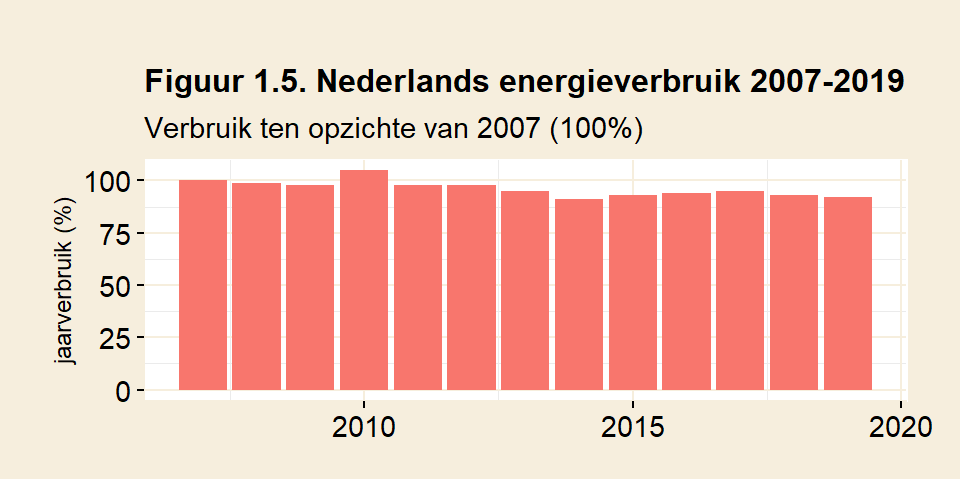
\includegraphics{02-Verbruik_files/figure-latex/unnamed-chunk-4-1} 

}

\end{figure}

\hypertarget{windenergie}{%
\chapter{Windenergie}\label{windenergie}}

Dit hoofdstuk schat de energieopbrengst en het ruimtegebruik van windmolens. Daarnaast wordt gekeken welk effect de onregelmatige opbrengsten uit wind hebben op de betrouwbaarheid van de energievoorziening.

\hypertarget{energie-uit-wind}{%
\section{Energie uit wind}\label{energie-uit-wind}}

Windmolens halen energie uit bewegende lucht. Meer wind betekent meer energie. De toename is exponentieel (de basisformule om dat te berekenen is \(\frac{1}{2} \rho v^3\) (\href{https://www.withouthotair.com/download.html}{MacKay}, p263. Zie ook bijlage A1)). Als de wind toeneemt van een windkracht twee (2 m/s) naar een windkracht drie (4 m/s) dan wordt de potentiële opbrengst verachtvoudigd, in plaats van verdubbeld. Een molen die staat op een plek waar het harder waait, ook al is dat weinig, wordt beloond.

Kijk eens naar figuur 2.1. Daar wordt de gemiddelde windsnelheid weergegeven voor een aantal meetmasten in Nederland (bron: \href{https://www.knmiprojects.nl/binaries/knmiprojects/documents/publications/2014/12/01/knmi-windkaart-van-100-m-hoogte/KNMI+-+Windkaart+van+100+m+hoogte.pdf}{KNMI, Windkaart van Nederland op 100m hoogte}). Voor alle masten geldt dat het op grotere hoogte harder waait. Eerste conclusie: hogere windmolens brengen meer op. Meetmast Cabauw staat op land, nabij Utrecht. OWEZ staat op zee. Interessant is dat het windprofiel op zee verschilt met dat in het binnenland. Boven land wordt de wind aan het oppervlak meer afgeremd. De windsnelheid neemt de eerste honderd meter snel toe, om daarna af te vlakken. Het is dus een goed idee om de molens op land in elk geval hoger dan 100m te maken. Op zee is het effect minder duidelijk.

\begin{figure}[t]

{\centering 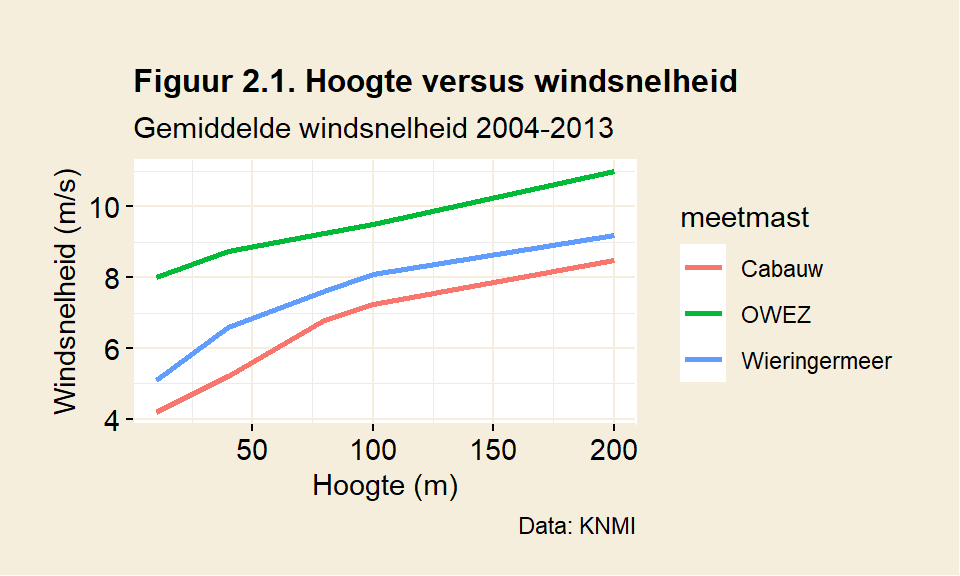
\includegraphics{03-Windenergie_files/figure-latex/hoogtevssnelheid-1} 

}

\end{figure}

De exponentiële toename van energie maakt het berekenen van de opbrengst van een windmolen er niet makkelijker op. Stel dat men de opbrengst over twee dagen wil berekenen. Op de eerste dag waait het 2 m/s en op de tweede dag 4 m/s. Omdat de windsnelheid in de formule tot de derde macht wordt verheven, is het middelen van windsnelheid niet zo'n goed idee. Rekent men met de gemiddelde windsnelheid (3m/s) dan geeft dat als uitkomst \(3^3 = 27\). Berekent men beide dagen apart, dan wordt de opbrengst hoger: \(\frac{2^3 + 4^3}{2} = 36\). Dit verschil neemt toe naarmate de periode waarover men middelt langer wordt.

Rekenen met de gemiddelde windkracht onderschat dus de totaalopbrengst. Het is beter om meetgegevens te gebruiken met een korte periode, in plaats van te rekenen met jaargemiddelden. Het KNMI heeft langjarige gegevens voorhanden die de windsnelheid in tijdsvakken van tien minuten weergeven (\href{https://dataplatform.knmi.nl}{KNMI Data Platform}). De berekeningen die volgen maken gebruik van deze fijnmazige data.

Figuur 2.2 laat de windsnelheid voor een heel jaar zien. De gebruikte data is afkomstig van KNMI's meetmast in Cabauw, nabij Utrecht. De metingen werden gedaan op 140 meter hoogte. Om de figuur enigzinds overzichtelijk te houden is de tienminutendata teruggebracht tot daggemiddelden. Hoewel dit de snelheidsverschillen afvlakt, is er duidelijk variatie in de windsnelheid te zien.

\begin{figure}[b]

{\centering 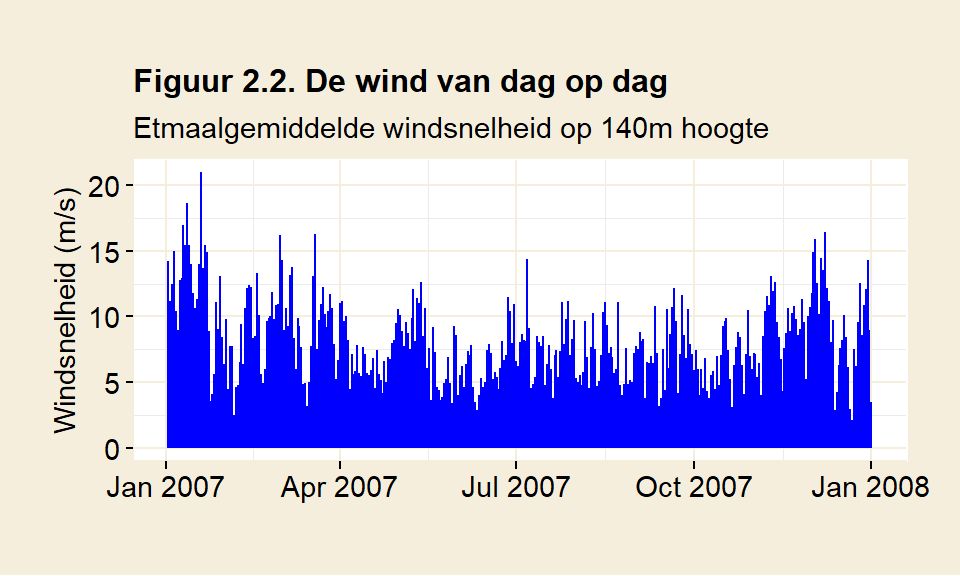
\includegraphics{03-Windenergie_files/figure-latex/wind2007-1} 

}

\end{figure}

De variatie in de windsnelheid wordt uitvergroot in de opbrengst. Verschil in windkracht leidt tot een nog groter verschil in opbrengst. Een exploitant van een windmolen moet rekening houden met pieken en dalen. Misschien geeft een bepaalde molen bij windkracht vier een mooie opbrengst. Deze windkracht staat er in werkelijkheid zelden. Bij een windkracht twee brengt de molen veel minder op. Bij een windkracht zes leidt het juist tot veel vermogen. Energietekorten, maar ook overschotten, worden zo uitvergroot. De uitschieters van 15 m/s in figuur 2.2 brengen in theorie zes keer meer op dan de gemiddelde windsnelheid over 2007 (8 m/s). Zakt de wind naar 4 m/s, dan blijft er slechts een achtste van de opbrengst over.

Windkracht heeft dus een grote invloed op de opbrengst van een molen. Verderop wordt ingegaan op hoe windsnelheid door een windmolen vertaald kan worden in opbrengst.

Daarnaast is er een tweede factor die grote invloed heeft op de opbrengst. Windmolens staan doorgaans bij elkaar, in een windpark. Molens die in elkaars buurt staan, vangen wind van elkaar af. De bovenwindse molens verstoren de lucht voor benedenwindse molens. Dat verlaagt de efficiëntie van het park.

Een belangrijke maat daarbij is de separatieafstand: de afstand tussen de molens in wiekdiameters. Om dezelfde separatie te behouden, moeten molens met grotere wieken verder uit elkaar worden geplaatst. Twee verschillende windparken met dezelfde separatieafstand zijn even efficiënt. De wiekdiameter van de gebruikte molen maakt daarbij niet meer uit. (Zie ook bijlage A1.)

Een alleenstaande molen heeft geen last van verstoring, en brengt dus meer op dan een molen in een park. Uit onderzoek van \href{https://www.researchgate.net/publication/230284417_Optimal_turbine_spacing_in_fully_developed_wind_farm_boundary_layers}{Meyers \& Meneveau} blijkt dat het efficiëntieverlies in een windpark een factor is om rekening mee te houden. \emph{Horns Rev} is een windpark op zee in Denemarken. Uit metingen daar blijkt dat een molen in het park slechts 60\% van de opbrengst realiseert in vergelijk met een alleenstaande molen. De molens in \emph{Horns Rev} hebben een separatieafstand van zeven wiekdiameters. Dat is \href{https://en.wikipedia.org/wiki/Wind_turbine\#Wind_turbine_spacing}{vrij normaal voor een windpark}. Uit het onderzoek van Meyers \& Meneveau blijkt dat een afstand van vijftien wiekdiameters optimaler zou zijn. Om de verstoring verwaarloosbaar te krijgen, moeten de molens op een afstand van meer dan honderd wiekdiameters staan.

Als windenergie een betekenisvolle bijdrage wil leveren, dan moet er rekening gehouden worden met dit efficiëntieverlies. Enkele windmolens op een dijk volstaan dan niet meer. De ruimte zal nuttig gebruikt moeten worden en dat betekent plaatsing in twee dimensies: een windpark.

Lees voor een uitgebreide beschrijving hoe de (theoretische) opbrengst uit windmolens berekend wordt bijlage A1.

\hypertarget{de-energieopbrengst-van-windmolens}{%
\section{De energieopbrengst van windmolens}\label{de-energieopbrengst-van-windmolens}}

Tot zover is het verhaal voornamelijk theoretisch. Nu nemen we een stapje richting de praktijk. Voor het berekenen van de opbrengst van windmolens gaat gebruik gemaakt worden van het opbrengstprofiel van een bestaande windmolen, de Enercon-126. Deze molen wordt bijvoorbeeld gebruikt in (\href{https://www.windparknoordoostpolder.nl/}{Windpark Noordoostpolder}), op de dijk bij Urk. Het zijn enorme molens. De doorsnede van de mast is bij de grond 14,5 meter. Daar kan een stadsbus ruim in geparkeerd worden. De molens zijn 200 meter hoog.

Een windmolen heeft in de praktijk een lagere opbrengst dan de theorie voorspelt. Er zijn in de praktijk natuurlijk efficiëntieverliezen, bijvoorbeeld door frictie in de aslagering, maar de grootste handicap is dat windmolens worden ontworpen op een bepaald windbereik. Binnen dat bereik is de molen efficiënt en wordt de theorie redelijk benaderd. Buiten dat bereik neemt de opbrengst snel af. (In bijlage A.2, \emph{windmolens in de praktijk}, wordt uitgebreid beschreven hoe de opbrengstberekening tot stand komt.)

Om de opbrengst van een windmolen te simuleren, wordt gebruik gemaakt van een opbrengstcurve (in dit geval van de Enercon-126, zie bijlage A2). Een opbrengstcurve geeft voor iedere windsnelheid weer hoeveel energie de molen kan leveren. Daarvoor kan de data van de KNMI worden gebruikt. Die geeft de gemiddelde windsnelheid over een tijdsvak van tien minuten. Uit de data wordt de windsnelheid op 140 meter hoogte gekozen, ongeveer de ashoogte van de Enercon-126. Aan de hand van de curve wordt dan vervolgens de opbrengst in het tijdsvak bepaald. Voor de berekening is aangenomen dat de windmolens onderling een separatieafstand hebben van 7 wiekdiameters. Dat brengt de efficiëntie van het windpark op 60\%. De opbrengst van het veld met windmolens wordt daarop aangepast.

\begin{figure}[t]

{\centering 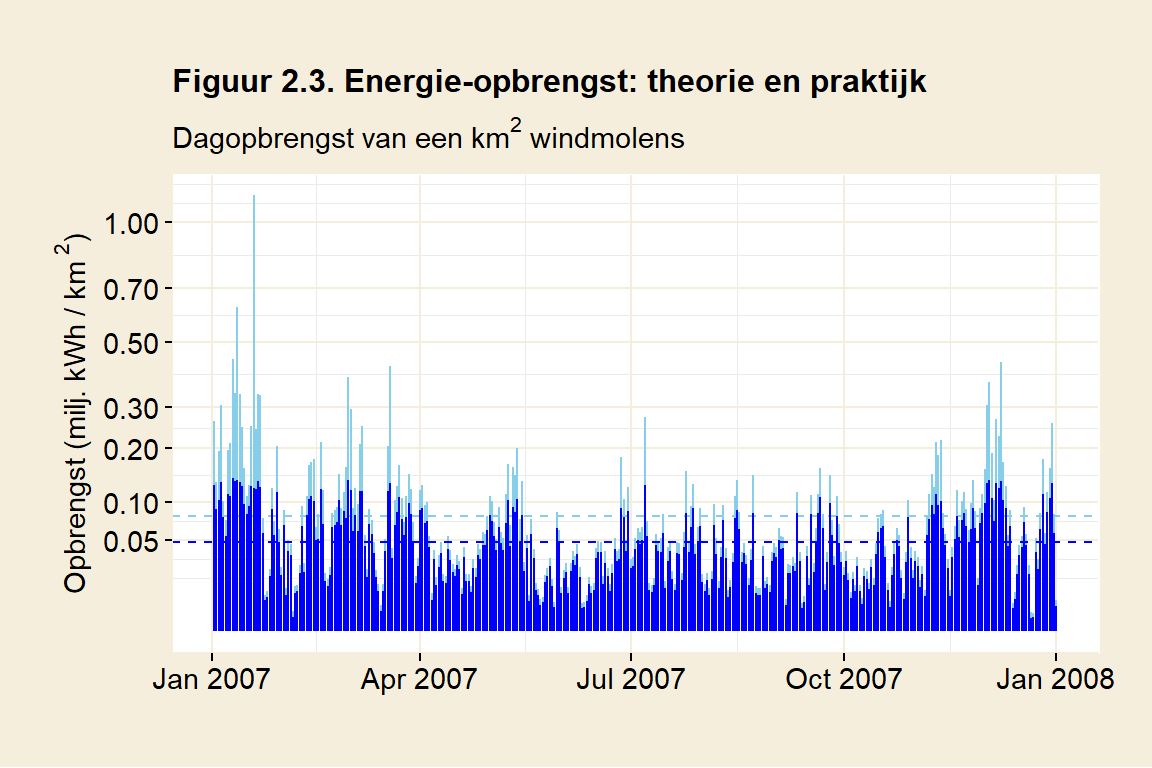
\includegraphics{03-Windenergie_files/figure-latex/Windopbrengst_theorie_en_praktijk-1} 

}

\end{figure}

De windsnelheden uit figuur 2.2 kunnen daarmee worden omgerekend in een energieopbrengst. Figuur 2.3 geeft die opbrengst weer. Zowel theorie als (gesimuleerde) praktijk worden getoond (Voor de berekening van de theoretische opbrengst, zie bijlage A1).

Op dagen met veel wind blijft de productie in de praktijk ver achter op de theoretische opbrengst (Let op: de schaalverdeling in figuur 2.3 is niet lineair. De verschillen lijken kleiner dan ze in werkelijkheid zijn). Vergelijk bijvoorbeeld eens de grootste dagopbrengst van de gesimuleerde Enercon-126 (in blauw) in figuur 2.3 met de theoretische opbrengst (in lichtblauw): 0.14 miljoen kWh per vierkante kilometer ten opzichte van 1.13 miljoen kWh. Het volle potentiëel kan niet worden gerealiseerd. Een windmolen in de praktijk brengt volgens deze berekening iets meer dan de helft op van een ideale windmolen (0.05 tegen 0.08 miljoen kWh per km\textsuperscript{2}). Je zou zeggen dat er dus ruimte voor verbetering is, maar dat valt tegen. Een ontwerper van een windmolen zit vast aan een bepaald windbereik. Huidige molens zijn \emph{in dat bereik} al heel efficiënt. Een grote verbetering in opbrengst valt dus niet te verwachten.

\hypertarget{ruimtegebruik}{%
\section{Ruimtegebruik}\label{ruimtegebruik}}

Figuur 2.3 toont een jaar met de dagopbrengsten van een vierkante kilometer met windmolens. Door alle dagen op te tellen, kan er een
jaaropbrengst worden berekend. Nu toont figuur 2.3 alleen 2007, zomaar een willekeurig jaar. Het nemen van een langere periode geeft een betere
schatting van gemiddelde jaaropbrengst. Als de computer de opbrengst berekent in de periode van 2006 tot en met 2015, dan blijkt de
gemiddelde jaaropbrengst uit te komen op 16 miljoen kWh per km\textsuperscript{2}.

Stel nu dat we \emph{alle} energie in Nederland zouden willen opwekken met wind. Daarbij wordt niet alleen het elektriciteitsgebruik, maar ook
fossiele brandstoffen meegenomen. Alles is gedekt: niet alleen gezinnen worden van energie voorzien, ook de gehele industrie, het vervoer, de
overheidsdiensten, alles. Dat verbruik kwam voor 2019 in totaal neer op 706 TWh, zoals werd toegelicht in hoofdstuk 1
(Verbruik).

In dit scenario is er dan, om Nederland van energie te voorzien, een oppervlakte van

\[ \frac {706 \; miljard\; kWh} {16 \;miljoen\;kWh / km^2} = 42966 \; km^2\]
\noindent nodig. Nederland beslaat \href{https://nl.wikipedia.org/wiki/Nederland}{41873 km\textsuperscript{2}}. Om energiedekkend te
worden met windenergie moet dan

\[ \frac {42966 \; km^2} {41873 \; km^2} = 103 \%\]
\noindent van Nederland ruimte bieden aan windmolens. Dat is meer landoppervlak dan Nederland heeft, en daarbij werden Waddenzee,
IJsselmeer en Zeeuwse stromen meegerekend. Op dit oppervlak zouden dan zo'n 54000
molens moeten staan. Het berekende oppervlakte is precies genoeg om Nederland van energie te voorzien, tenminste als men fluctuaties in de
energievoorziening buiten beschouwing laat.

Windmolens kunnen ook op zee worden geplaatst. De KNMI heeft daar helaas geen fijnmazige data voorhanden, dus het is hier niet
berekend. Een grove schatting van de opbrengst valt te geven door te kijken naar het verschil in windsnelheid tussen land en zee. Daarvoor
kan figuur 2.1 worden gebruikt. Op 140m hoogte heeft OWEZ, de locatie op de noordzee, een gemiddelde windsnelheid van
10.1 m/s. Cabauw geeft voor de zelfde hoogte
7.8 m/s. Op zee zou men dan een twee keer grotere opbrengst verwachten (10.1\textsuperscript{3} /
7.8\textsuperscript{3} =
2.2), aangenomen dat de windfluctuaties ongeveer
hetzelfde zijn op beide locaties.

De installatie zou in dat geval met de helft kunnen worden verkleind. Volgens een \href{https://nl.wikipedia.org/wiki/Windturbines_in_Nederland}{schatting op
wikipedia} is 40\% van het continentale plat, oftewel 23.000 km\textsuperscript{2}, beschikbaar voor
plaatsing van windmolens. Het continentale plat zou dan ongeveer volgeplaatst zijn, in het geval alle energie van zeewind zou komen.

Plaatsing op zee heeft wel zijn eigen uitdagingen. De zee vormt een corrosieve omgeving waardoor het onderhoud toeneemt. De bereikbaarheid
is aanzienlijk slechter dan op land. Deze zaken zorgen ervoor dat windmolens op zee duur zijn. Volgens de US Energy Information
Administration is wind op zee bijna drie keer duurder dan op land, drie keer duurder dan gascentrales, en anderhalf keer duurder dan kernenergie
(\href{https://www.eia.gov/outlooks/aeo/pdf/electricity_generation.pdf}{EIA Annual Energy Outlook 2020, tabel 1b, pg7}).

\hypertarget{opbrengstfluctuaties}{%
\section{Opbrengstfluctuaties}\label{opbrengstfluctuaties}}

Als heel Nederland voorzien wordt van windmolens kan er dus \emph{gemiddeld} gezien aan ons energieverbruik worden voldaan. Daarmee zijn we er echter nog niet. Wat gebeurt er met de energievoorziening als het niet waait? Dan zit Nederland zonder energie. Perioden met weinig wind veroorzaken een energietekort. Energie zal op die momenten prijzig worden. Er moet worden gekozen wie recht heeft op energie in tijden van krapte. Dat wil men waarschijnlijk voorkomen. Het is dus belangrijk om een beeld te krijgen van de grootte van de energietekorten.

Figuur 2.5 geeft de maandopbrengsten weer van een fictief park met windmolens met de
opbrengstkarakteristieken van de Enercon-126. Hierin is aangegeven welke maanden een overschot hebben en in welke maanden er een tekort onstaat. Groene maanden geven een bovengemiddelde opbrengst aan, rode maanden een opbrengst onder het gemiddelde. De aanname hierbij is dat Nederland iedere maand een constante hoeveelheid energie gebruikt en dat de gemiddelde opbrengst van de windmolens de vraag dekt. De rode stippellijn geeft de energievraag aan.

\begin{figure}[!t]

{\centering 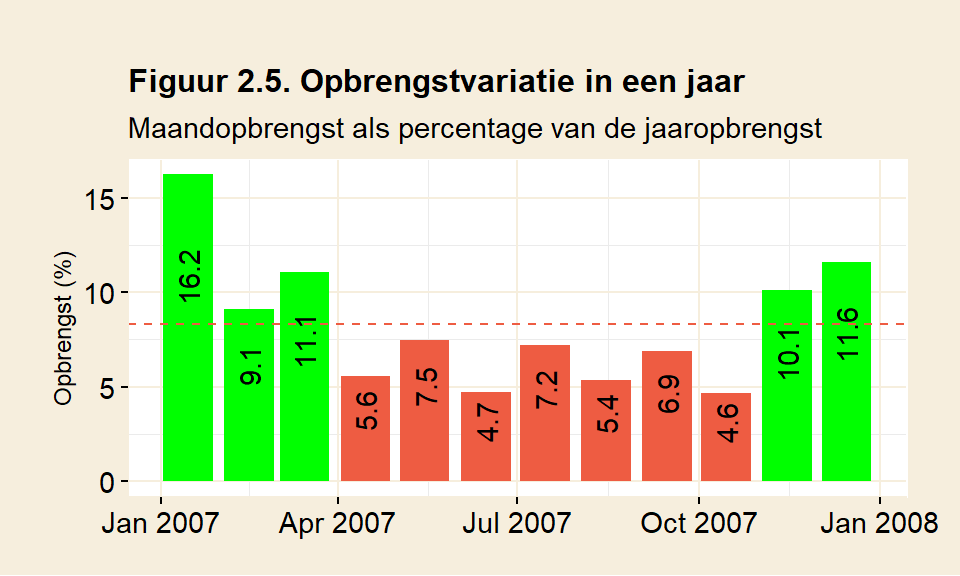
\includegraphics{03-Windenergie_files/figure-latex/opbrengstvariatie2007-1} 

}

\end{figure}

De maandopbrengst wordt weergegeven in procenten van de totale jaaropbrengst. In een gemiddelde maand mag er dus een opbrengst van \(\frac{100 \%}{12} = 8\frac{1}{3}\%\) verwacht worden. In 2007 is te zien dat er in januari t/m maart en in november en december overschot is: er wordt meer dan gemiddeld geproduceerd. Schaarste ontstaat in de zomerperiode, van april t/m oktober. Dan onstaat er een tekort ten opzichte van het gemiddelde. Er is een seizoenseffect te zien dat kenmerkend is voor wind: in de wintermaanden is de productie duidelijk groter dan in de zomer. Dat is niet ongewoon, de meeste jaren kennen dit patroon.

Hoe groot is het overschot? Neem januari. Januari genereert 16.2\% van de totale jaaropbrengst. In januari kan
er dus bijna twee keer meer geproduceerd worden dan het gemiddelde van \(8\frac{1}{3}\)\%. Tekorten zijn er ook. Neem oktober, dat een opbrengst heeft van 4.6\%. Ten opzichte van het gemiddelde wordt er nu slechts de helft geproduceerd. De opbrengstverschillen zijn dus aanzienlijk.

Het kijken naar maandgemiddelden geeft een duidelijk beeld van seizoensvariaties. De variatie binnen een maand blijft zo echter verborgen. Ook een maand met gemiddelde opbrengst kan best een week hebben waarin het niet waait. Figuur 2.6 laat zien hoe dat verliep voor maart van 2007. Maart is meestal een maand met op zich voldoende opbrengst, deze maart in 2007 brengt iets meer dan gemiddeld op. Figuur 2.6 belicht de opbrengstvariatie van dag op dag.

\begin{figure}[b]

{\centering 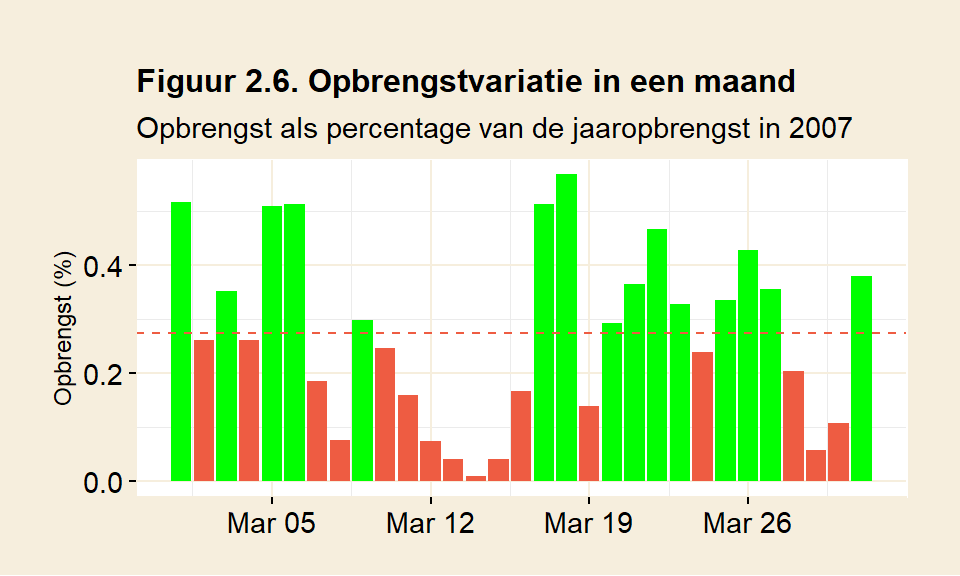
\includegraphics{03-Windenergie_files/figure-latex/opbrengstvariatie2007.d-1} 

}

\end{figure}

Er zijn vier dagen in maart te zien waarin de opbrengst vrijwel nihil is: in de periode van 12 t/m 15 maart wordt weinig geproduceerd. Op 14 maart is er een dagtekort van 96\%: het waait bijna niet. Op deze dag moet de energie dus bijna in z'n geheel ergens anders vandaan komen.

\hypertarget{windarme-maanden}{%
\subsection{Windarme maanden}\label{windarme-maanden}}

In 2007 was maart een windrijke maand, met bovengemiddelde opbrengst. Maanden met overschot zijn het minst problematisch, hoewel ook variatie binnen een maand best een dagenlang tekort kan veroorzaken. De grootste tekorten zijn echter te verwachten in maanden met een ondergemiddelde opbrengst. Dat zijn vaak de zomermaanden. Figuur 2.7 laat juni in 2018 zien, een willekeurige zomermaand. De opbrengst wordt fijnmazig weergegeven, iedere staaf vertegenwoordigt tien minuten in deze maand.

\begin{figure}[t]

{\centering \includegraphics{03-Windenergie_files/figure-latex/opbrengstvariatie2018j-1} 

}

\end{figure}

De fijnmazigheid laat goed zien hoeveel variatie zo'n windmaand eigenlijk heeft. De rode stippellijn vertegenwoordigt de gemiddelde energievraag in 2018 voor een tijdsvak van 10 minuten (ongeveer 0,002\% van de jaaropbrengst). Duidelijk is dat veel tijdsvakken onvoldoende opbrengen, namelijk onder de rode stippellijn. Vaak blijft de opbrengst ver onder het gemiddelde. In de eerste tien dagen van de maand komt de opbrengst tot 28\% van de gemiddelde energievraag. Een groot gedeelte van het energieverbruik, namelijk 72\%, zal in deze periode dus moeten worden aangevuld.

Er zijn ook regelmatig perioden met windstiltes te tellen: op het oog zijn er een paar te onderscheiden. Telt de computer, dan is het in totaal 16\% van de tijd windstil (gedefinieerd als minder dan een twintigste van de gemiddelde opbrengst). Er zijn ook langere perioden van meer dan een week waarin het structureel minder waait.

Hier werden twee vrij willekeurige maanden bekeken; er is niet speciaal gezocht naar de maand met de minste opbrengst. Historische gegevens zijn bruikbaar voor een algemene indruk. Dat betekent niet dat er zich in de toekomst geen grotere extremen kunnen voordoen. Eigenlijk moet er bij de inschatting van mogelijke perioden met tekorten dus nog extra marge ingecalculeerd worden voor extreme weerssituaties.

\bigskip\noindent Wat betekenen deze overschotten en tekorten? Stel, men zet een bepaald windpark neer gebaseerd op het aantal kilowattuur dat men per jaar wil produceren. Hoewel er voldoende capaciteit is, kan er niet altijd aan de energievraag worden voldaan. Op die momenten zal de energie ergens anders vandaan moeten komen.

Op dit moment voorziet windenergie volgens het CBS in ruim één procent van onze energiebehoefte (Zie figuur 1.2, in hoofdstuk 1). Gebrek aan wind kan makkelijk worden opgevangen door fossiele energiecentrales het tekort te laten aanvullen. Het aandeel van windenergie is immers nog niet zo groot en de energiecentrales staan er toch al.

Naarmate windenergie in aandeel groeit, worden deze tekorten echter vervelender. Essentiële afnemers zoals ziekenhuizen moeten op ieder moment bediend kunnen worden, maar ook voor andere afnemers geldt dat afname op het moment dat zij het nodig hebben essentiëel is voor hun economisch functioneren. Hoe stellen we de energievoorziening zeker met een fluctuerende bron zoals windenergie?

\hypertarget{fluctuaties-opvangen-met-opslag}{%
\section{Fluctuaties opvangen met opslag}\label{fluctuaties-opvangen-met-opslag}}

Een optie is om de fluctuaties op te vangen door middel van energieopslag. Die kan gebruikt worden om overschotten en tekorten te vereffenen. Overproductie van energie kan worden bewaard; in tijden van schaartste kan de opslagen energie worden geleverd aan gebruikers. Energie zou kunnen worden opgeslagen in bijvoorbeeld accu's, in waterstof of in spaarbekkens. Om hoeveel energie gaat het dan eigenlijk? Hoe kan worden ingeschat hoe groot deze opslag zou moeten zijn? Om dat te kwantificeren wordt hier gekeken naar het grootste cumulatieve tekort over een bepaalde periode.

In figuur 2.5 kan men een lange windarme periode zien, lopend van april tot en met oktober. April vormt de eerste maand met een tekort (8,3\% - 5,6\% = 2,7\%) en in de daaropvolgende maanden loopt het tekort verder op. In totaal ontstaat zo een `lopend' tekort in dit jaar van 16.5\% (zie bijlage A.4,
\emph{berekenen van lopend tekort} voor een nadere uitwerking). Dat betekent dat, om de fluctuaties in de stroomproductie voor dit jaar op te vangen, er opslag ter grootte van 16.5\% van de jaarproductie voorhanden had moeten zijn. Een `accu' ter grootte van 16.5\% van het jaarverbruik had de tekorten kunnen opvangen, tenminste als de `accu' bij aanvang voldoende gevuld was.

Het tellen van het tekort in figuur 2.5 geeft een eerste indruk, maar een beter beeld wordt verkregen door een langere periode te bekijken. In figuur 2.8 wordt tien jaar windenergie gesimuleerd in combinatie met opslag. Er wordt een denkbeeldige accu gebruikt om windenergie in op te slaan en tekorten te kunnen aanvullen. Er wordt weer uitgegaan van een windmolenpark dat voldoende opbrengst heeft om gemiddeld gezien aan de vraag te voldoen, en dat deze energievraag constant is.

Om het overzichtelijk te houden, geeft de figuur maandtotalen. De berekeningen gaan zoals eerder uit van kortere perioden van tien minuten. Per tien minuten kunnen zich twee situaties voordoen.

\begin{enumerate}
\def\labelenumi{\arabic{enumi}.}
\tightlist
\item
  \emph{Er is meer windenergie dan er vraag is}. Het surplus wordt bewaard
  in de opslag (de lichtgroene staven in de figuur). Het andere deel
  van de opgewekte windenergie wordt direct door afnemers gebruikt (\emph{wind}, de groene staven in de figuur).
\item
  \emph{Er is te weinig wind om aan de vraag te voldoen}. Nu moet er
  energie uit de opslag worden gebruikt om het tekort aan te vullen
  (\emph{aangevuld}, de donkergroene staven in de figuur). De opgewekte
  windenergie wordt ook onthouden en komt in de groene staven terecht.
\end{enumerate}

\begin{figure}[!t]

{\centering 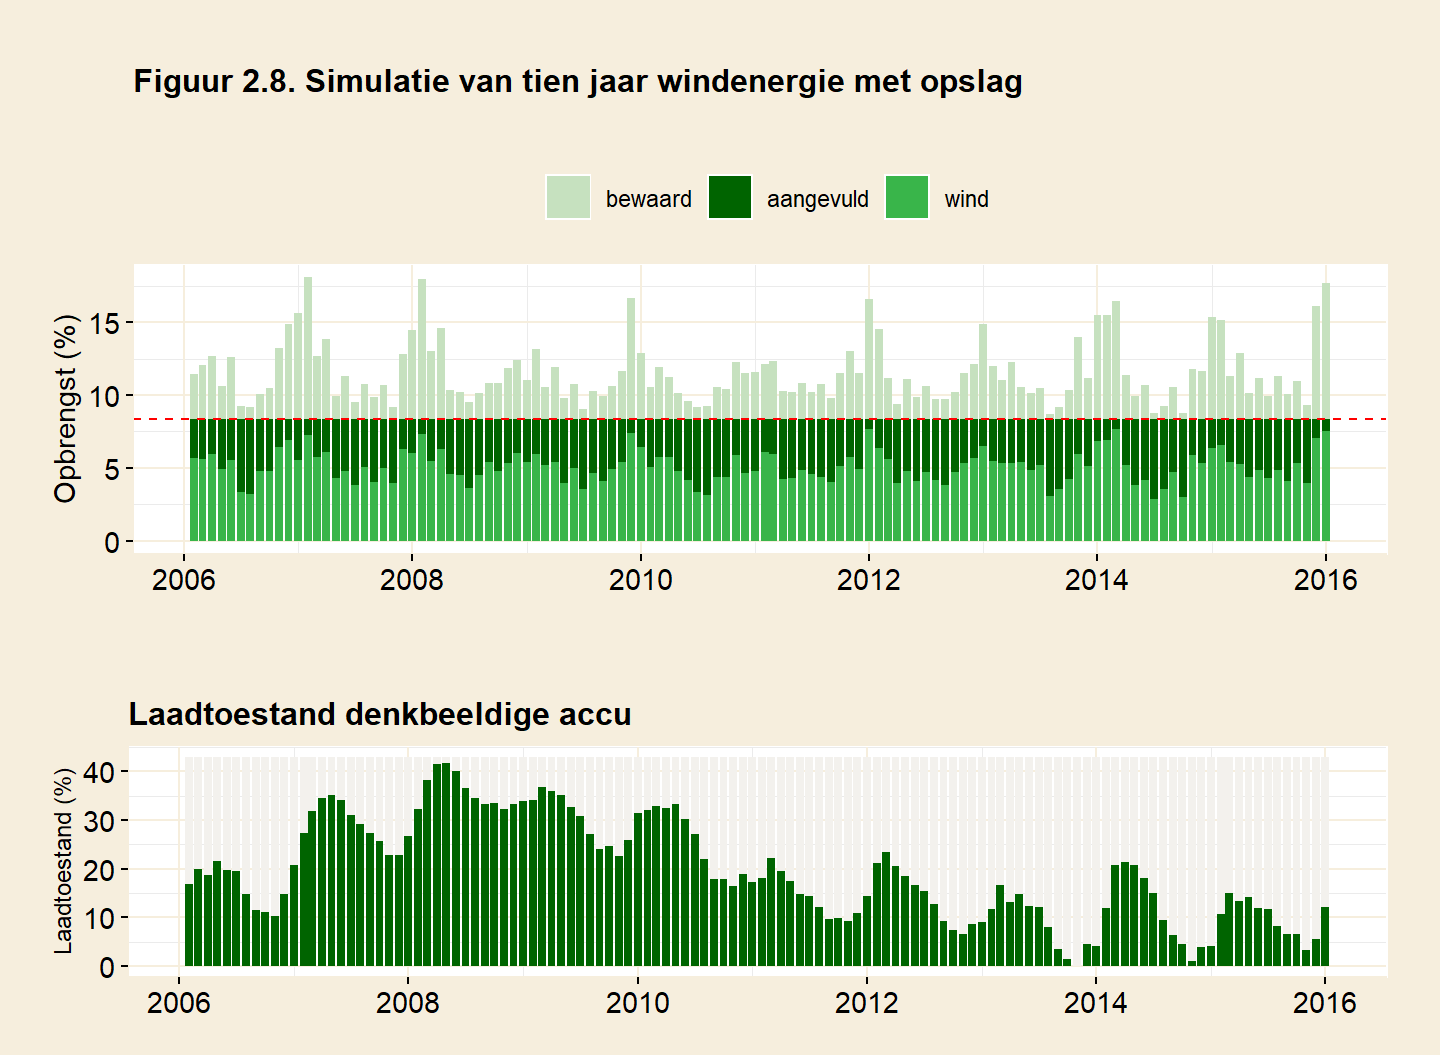
\includegraphics{03-Windenergie_files/figure-latex/infographic_opslag-1} 

}

\end{figure}

\noindent
In figuur 2.8 is te zien dat iedere maand netjes wordt voldaan aan de vraag: de directe productie uit wind plus energie aangevuld uit de accu reikt precies tot de rode stippellijn. Het probleem van de niet-continue opbrengst is dus opgelost. Overproductie uit wind wordt steeds bewaard in de accu. In een maand met een overschot aan wind neemt de laadtoestand van de accu toe. In een maand met tekort neemt de laadtoestand af. Over het algemeen zorgt de winterperiode voor het laden van de accu, terwijl er in zomerperiode vooral wordt ontladen. Dat is te zien aan het golfpatroon in het verloop van de laadtoestand.

De accu lijkt in 2006 te starten op een vrij willekeurige laadtoestand, ergens boven de 15\% van het jaarverbruik. Dat heeft te maken met het feit dat de accu eind 2013 nét leegraakt. Een hogere beginstand--en daarmee een ruimere accu--had ook gewerkt, maar deze benadering geeft ons de minimale benodigde opslagcapaciteit: 44\% van het jaarlijks energieverbruik (307 TWh). Dat komt neer op een opslag ter grootte van 5 maanden nationaal verbruik.

Dat is aanzienlijk meer dan berekend in het eerdere voorbeeld (16,5\% voor alleen 2007). Dat komt omdat de berekening van tekorten nu over een langere periode wordt gedaan. Als een tekort in de winterperiode niet helemaal weer wordt aangevuld, kan deze in de loop van tijd uitdiepen. Hier gebeurt dat in de periode tussen 2008 en 2014. De accu raakt gedurende deze 10 jaar steeds leger. De zomers zijn niet meer genoeg om de accu te vullen. De capaciteit van 44\% is genoeg om \emph{deze} tien jaar te dekken, maar de vraag is hoeveel jaar dat nog goed zou gaan. De steeds leger wordende accu is een indicatie dat deze waarschijnlijk te klein is voor de taak.

\hypertarget{fluctuaties-opvangen-met-een-hulpbron}{%
\section{Fluctuaties opvangen met een hulpbron}\label{fluctuaties-opvangen-met-een-hulpbron}}

Naast opslag is er een tweede manier om tekorten op te vangen. Er kan een alternatieve energiebron worden aangesproken. De bron wordt \emph{stand-by} gehouden totdat er vraag optreedt. In principe komt iedere bron die in staat is om snel te reageren op de vraag in aanmerking. Daarbij kan bijvoorbeeld gedacht worden aan gas- of kerncentrales. Opslag wordt hier nu buiten beschouwing gelaten.

In figuur 2.9 wordt weer tien jaar windenergie gesimuleerd, waarbij ditmaal een hulpbron wordt gebruikt om tekorten aan te vullen. Ook hier kunnen er zich per tien minuten twee situaties voordoen, ditmaal met andere gevolgen.

\begin{figure}[!t]

{\centering \includegraphics{03-Windenergie_files/figure-latex/infographic_hulpbronnen-1} 

}

\end{figure}

\begin{enumerate}
\def\labelenumi{\arabic{enumi}.}
\tightlist
\item
  \emph{Er is meer windenergie dan er vraag is}. Het surplus gaat verloren,
  want in dit scenario is er geen opslag (\emph{ongebruikt}, de grijze staven in de figuur). Het andere
  deel van de opgewekte windenergie wordt direct door afnemers gebruikt (\emph{wind}, de groene staven in de
  figuur).
\item
  \emph{Er is te weinig wind om aan de vraag te voldoen}. Nu moet er worden
  bijgedraaid door de hulpbron om het tekort aan te vullen (de
  blauwe staven in de figuur). Ook hier komt de opgewekte
  windenergie in de groene staven terecht.
\end{enumerate}

\noindent Het volgende beeld onstaat. Door de hulpbron energie bij te laten draaien kan iedere maand inderdaad precies aan de energiebehoefte van Nederland worden voldaan. Windenergie (groen) en hulpbron (blauw) tezamen komen uit op de stippellijn: het verbruik van Nederland. Tevens is te zien dat er windenergie onbenut blijft, de grijze staven. Een maand kan zowel overschot (grijs) als tekort (blauw) bevatten. In iedere maand zijn er vele perioden van tien minuten te vinden met een overschot, en anderen juist weer met een tekort.

In dit scenario blijkt windenergie 61\% van de jaarlijkse energievraag te leveren en de hulpbron moet dus 39\% van de benodigde energie bijdraaien.

Er zit nog een andere kant aan het gebruik van een hulpbron. Er zullen momenten zijn dat het helemaal niet waait, zoals bijvoorbeeld op 14 maart 2007. Op zo'n moment moet de hulpbron de volledige last van de vraag dragen. Dat wil zeggen dat het vermogen van de hulpbron in staat moet zijn de maximale energievraag te dekken. Deze hoeveelheid vermogen vertaalt zich in het aantal energiecentrales. Zelfs al zou er maar weinig wordt geleverd door de hulpbron op jaarbasis, kan men niet af met `een paar' gas- of kerncentrales: men zal een installatie moeten hebben staan die de volledige vraag van Nederland kan dekken.

\hypertarget{zonne-energie}{%
\chapter{Zonne-energie}\label{zonne-energie}}

Het doel van dit hoofdstuk is een schatting te geven van de energie-opbrengst en het ruimtegebruik van zonne-energie. Daarnaast wordt gekeken naar de gevolgen van fluctuaties in de opbrengst van zonne-energie.

\hypertarget{variatie-in-zonneschijn}{%
\section{Variatie in zonneschijn}\label{variatie-in-zonneschijn}}

Figuur 3.1 laat op dagbasis zien hoeveel straling Nederland in 2007 ontving, hetzelfde jaar als er bij wind werd gekozen. Het lijkt een jaar te zijn met een vrij slechte zomer (weinig zon), maar het algemene beeld is vergelijkbaar met andere jaren. Op de breedtegraad van Nederland varieert de invalshoek van de zonnestraling gedurende het jaar aanzienlijk. De zon staat hoog aan de hemel in de zomer en laag in de winter. Dat is te zien aan de golfbeweging in de grafiek, die een beetje een sinusoïde vorm heeft. Het seizoenseffect is groot en tegelijkertijd regelmatig. Het andere regelmatige ritme wat betreft de intensiteit van de straling, niet zichtbaar in deze grafiek, is natuurlijk het dag-nachtritme. 's Nachts is er geen straling te verwachten; op het midden van de dag het meeste. Tot zover is het allemaal heel voorspelbaar.

\begin{figure}[!b]

{\centering 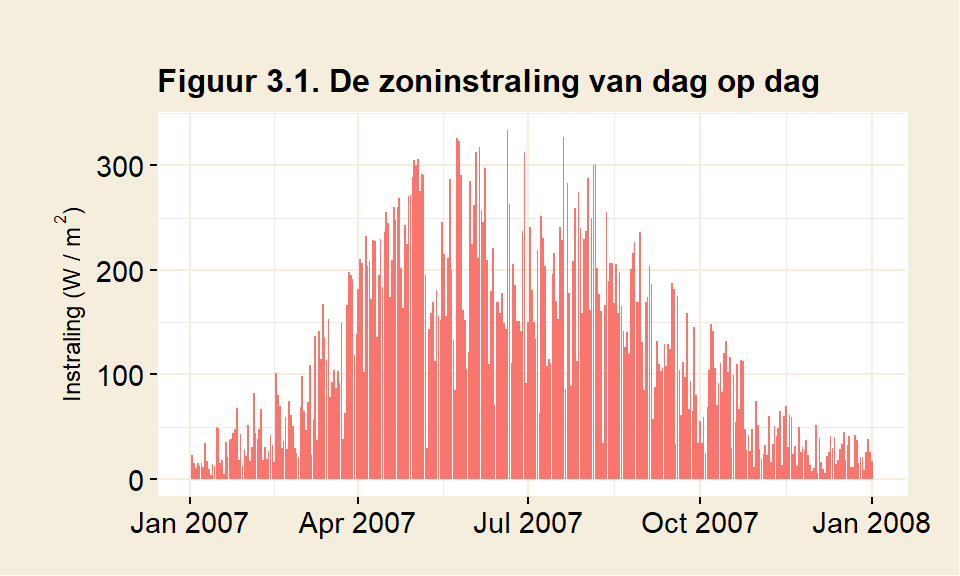
\includegraphics{04-Zonne-energie_files/figure-latex/zon2007-1} 

}

\end{figure}

Figuur 3.1 laat ook zien dat er, hier met name in de zomer, flinke gaten vallen in de hoeveelheid ontvangen zonnestraling. Dat heeft te maken met het weer. Bewolking heeft een grote invloed op de opbrengst van zonnecellen. Als het bewolkt is, is het niet ongewoon dat een zonnecel maar een tiende levert van wat deze in volle zon zou leveren (\href{https://www.withouthotair.com/download.html}{MacKay}, p45). Het weer kan dus een grote invloed hebben op de opbrengst van zonnecellen.

\hypertarget{de-energie-opbrengst-van-zonnecellen}{%
\section{De energie-opbrengst van zonnecellen}\label{de-energie-opbrengst-van-zonnecellen}}

Zonnecellen zetten straling om in elektriciteit. De relatie tussen energie-opbrengst van zonnecellen en de instralingswaarden zoals deze bijvoorbeeld door het KNMI worden gegeven, is betrekkelijk eenvoudig. De opbrengst is gelijk aan het rendement van het zonnepaneel maal de hoeveelheid ingevallen straling. Heeft een bepaald soort zonnecellen bijvoorbeeld een rendement van 20\% en is de hoeveelheid ingevallen straling gelijk aan 1100 kWh per m\textsuperscript{2} per jaar, dan zal een vierkante meter van deze zonnecellen in een jaar 220 kWh opbrengen. In tegenstelling tot wind is de relatie tussen straling en opbrengst bij zon lineair. Dat maakt de zaak een stuk eenvoudiger.

Een belangrijke vraag is daarmee welk rendement er voor zonnecellen verwacht mag worden. Een hoger rendement bepaalt de hoeveelheid oppervlak dat voor zonnecellen nodig is. Voor de \emph{variatie} in de opbrengst maakt het niet uit, die blijft hetzelfde of er nu meer of minder efficiënte zonnecellen worden gebruikt.

Gewone zonnepanelen, zoals die nu beschikbaar zijn, zijn gevoelig voor licht van slechts één bepaalde golflengte (het paneel bestaat uit zogenaamde enkelvoudige of \emph{single-junction} cellen). Het maximaal theoretisch rendement van een enkelvoudige cel is gebonden aan de \href{https://en.wikipedia.org/wiki/Shockley\%E2\%80\%93Queisser_limit}{Shockley-Queisser limiet} van ongeveer 34\%. Commerciële cellen halen nu tot 24\% rendement. Dat is al dicht in de buurt van de te verwachten praktische limiet van \href{https://en.wikipedia.org/wiki/Solar_cell}{ongeveer 26\%}.

Er bestaan ook cellen met \href{https://en.wikipedia.org/wiki/Multi-junction_solar_cell}{meervoudige juncties} die een hoger rendement hebben dan cellen met een enkelvoudige junctie. Deze cellen bestaan uit verschillende materialen, waardoor er in principe uit verschillende golflengtes energie kan worden gewonnen. De theoretische limiet, bij een stapeling van een oneindige hoeveelheid lagen, is zo'n 69\%. Het beste gerealiseerde rendement tot nu toe is 47\%, maar daarbij werd zonlicht geconcentreerd. Het concentreren kost ruimte: een hoger rendement betekent dan ook niet automatisch een hogere opbrengst per vierkante meter. Zie \href{https://en.wikipedia.org/wiki/Solar_cell_efficiency}{wikipedia/ solar cell efficiency} en verdere verwijzingen daarin.

\bigskip\noindent
Voordat er gesproken kan worden over opbrengst, moet er gekozen worden van welk rendement er moet worden uitgegaan. De keuze zal ergens moeten liggen tussen de theoretische limiet van 69\% voor meervoudige zonnecellen en 6\% voor goedkope silicium-gebaseerde zonnecellen. Bij de berekeningen hier wordt uitgegaan van (duurdere) zonnecellen met een rendement van 20\% (zie ook bijlage B.1 \emph{Berekenen van opbrengst}). Dat zijn zonnecellen met een hoog rendement, weliswaar duur, maar wel algemeen beschikbaar.

De instralingsgegevens van het KNMI uit figuur 3.1 kunnen gebruikt worden om de opbrengst te berekenen van een vierkante kilometer zonnecellen. Er wordt van uitgegaan dat de zonnecellen tegen elkaar aan geplaatst worden, zonder enige tussenruimte. Figuur 3.2 toont deze energieopbrengst.

\begin{figure}

{\centering 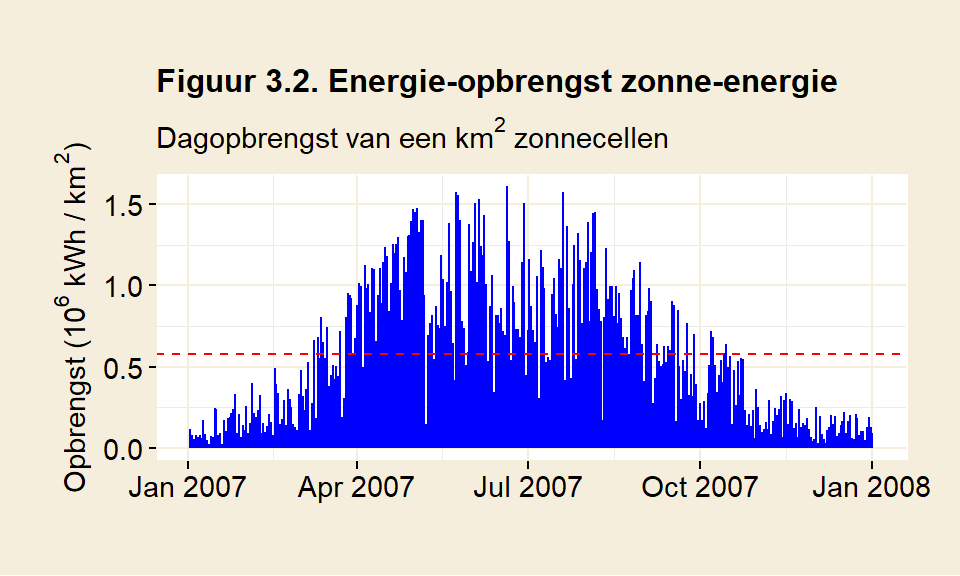
\includegraphics{04-Zonne-energie_files/figure-latex/opbrengstzon2007-1} 

}

\end{figure}

De zonnestraling die Nederland ontvangt is volgens het \href{https://www.knmi.nl/over-het-knmi/nieuws/zonnestraling-in-2019}{KNMI} doorgaans rond 1000 à 1100 kWh per m\textsuperscript{2} per jaar. De berekende jaaropbrengst voor 2007, getoond in figuur 3.2, komt uit op 211 kWh voor een vierkante meter zonnepaneel. Voor een zonnepaneel met een effciëntie van 20\% komt dat mooi in de buurt voor een gemiddelde instraling van iets boven de 1000 kWh. Het gebruik van een efficiënter paneel zou de opbrengst in figuur 3.2 verhogen, maar de vorm van de grafiek niet veranderen. Met andere woorden: de hoeveelheid fluctuatie blijft gelijk.

\hypertarget{ruimtegebruik-1}{%
\section{Ruimtegebruik}\label{ruimtegebruik-1}}

Laten we, net zoals bij windenergie werd gedaan, een denkbeeldig scenario nemen om een inschatting te kunnen maken van de hoeveelheid benodigde ruimte voor zonnecellen. Stel dat alle energie die Nederland gebruikt weer door een duurzame bron wordt opgewekt, ditmaal door zonne-energie.

Net zoals bij wind wordt ook hier weer een periode van 10 jaar gebruikt, van 2006 tot en met 2015. Aan de hand van de gegevens van het KNMI wordt iedere 10 minuten, op basis van de straling in dat tijdsvak, de energie-opbrengst uitgerekend van een vierkante kilometer zonnecellen (belegd met panelen met een rendement van 20\%). Als in deze periode van 10 jaar alle opbrengsten bij elkaar worden opgeteld en vervolgens een jaargemiddelde wordt berekend, dan volgt daaruit een opbrengst van 218 miljoen kWh per km\textsuperscript{2}.

Dan kan nu worden berekend hoeveel ruimte er nodig zou zijn in een scenario waarbij Nederland al zijn energie opwekt met behulp van de zon. Er wordt daarbij wederom vanuit gegaan dat de panelen zonder tussenruimte tegen elkaar aan geplaatst worden. Het totale energieverbruik van Nederland in 2019 was 706 miljard kWh (zie hoofdstuk 1).

Hoeveel vierkante kilometer zonnepanelen zou er nodig zijn om het gehele energiegebruik van Nederland te dekken? Daarvoor delen we ons energieverbruik door de opbrengst van zonne-energie per vierkante kilometer:

\[ \frac {706\; miljard \; kWh} {218 \; miljoen \; kWh/km^2} = 3237 \; km^2  \]
\noindent
Deelt men het oppervlak benodigd voor zonnecellen door het oppervlak van Nederland dan blijkt dat

\[ \frac {3237 \; km^2} {41873 \; km^2} = 7.7 \% \]
\noindent
van Nederland nodig is om ons hele energieverbruik te dekken. Dat is grofweg de grootte van de provincie Zuid-Holland. Daarmee is zonne-energie veel efficiënter dan windenergie. De opbrengst per vierkante kilometer is veel hoger.

\hypertarget{opbrengstfluctuaties-1}{%
\section{Opbrengstfluctuaties}\label{opbrengstfluctuaties-1}}

De opbrengst van een zonnecel varieert met de hoeveelheid ingevallen straling op een bepaald moment. Bij windenergie bleek deze variatie tot substantiële tekorten te leiden. Hoe zit dat bij zon?

Figuur 3.3 geeft de opbrengstvariatie weer op maandbasis voor het jaar 2007. De aanname daarbij is weer dat Nederland iedere maand een gelijke hoeveelheid energie gebruikt en de panelen over het hele jaar genomen de vraag dekken.

\begin{figure}[t]

{\centering 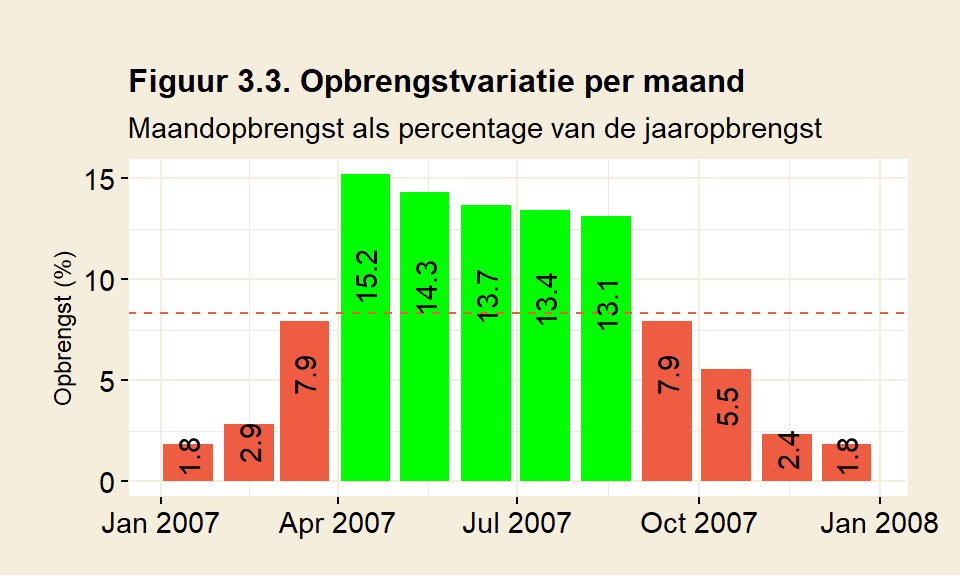
\includegraphics{04-Zonne-energie_files/figure-latex/opbrengstvariatiezon2007-1} 

}

\end{figure}

Er blijkt een duidelijk seizoenseffect uit figuur 3.3. Het is een beetje een ongewoon jaar in de zin dat de meeste opbrengst niet in juni en juli valt, hetgeen aangeeft dat ook weersinvloeden een factor van belang zijn. In tegenstelling tot wind is hier zoals verwacht de zomer de beste periode. In de winter zakt de opbrengst daarentegen tot ver onder het gemiddelde. Januari brengt 1.8\% op, dat is 78\% minder dan gemiddeld. Mei is een maand met overvloed, hier kan 72\% meer dan gemiddeld worden geproduceerd.

Figuur 3.3 maakt de seizoensinvloeden inzichtelijk, maar de opbrengstvariatie die binnen een maand optreedt blijft verborgen. Figuur 3.4 toont de opbrengst op dagbasis voor de maand september in 2007. In totaal had deze maand een (bijna) gemiddelde opbrengst, dus in principe dekkend voor het energieverbruik in die maand.

\begin{figure}[b]

{\centering 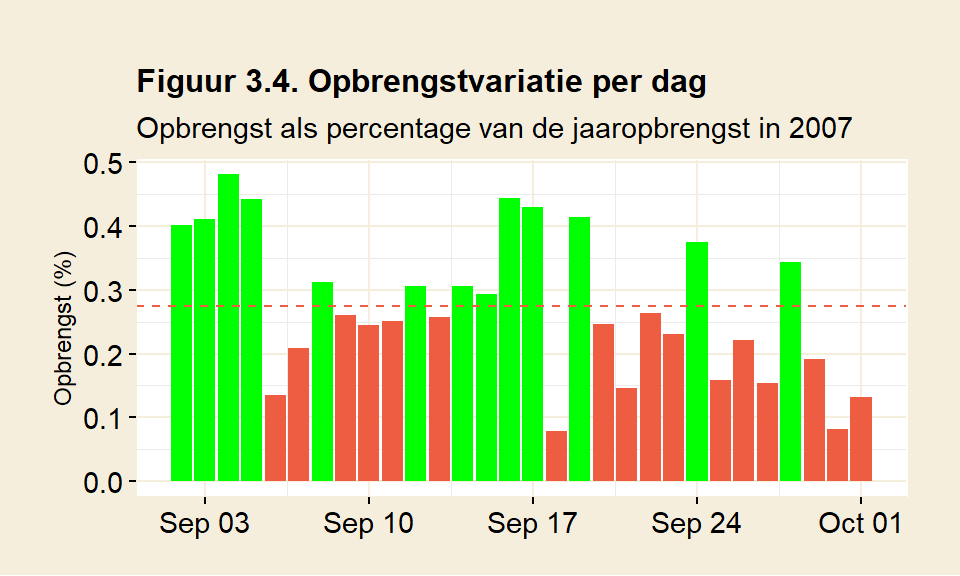
\includegraphics{04-Zonne-energie_files/figure-latex/opbrengstvariatiezon2007.d.plot-1} 

}

\end{figure}

Figuur 3.4 laat echter zien dat de maand september zelf op dagbasis nog aanzienlijke variatie kende. In deze september waren er 6 dagen waar er ruim 50\% meer dan gemiddeld kon worden geproduceerd. Omgekeerd kwam er op 4 dagen in deze maand minder dan de helft van het gemiddelde binnen.

\hypertarget{zonarme-maanden}{%
\subsection{Zonarme maanden}\label{zonarme-maanden}}

\begin{figure}[b]

{\centering \includegraphics{04-Zonne-energie_files/figure-latex/opbrengstvariatie2018j-1} 

}

\end{figure}

De grootste tekorten zijn te verwachten in maanden met weinig zon. Dat is doorgaans in de winter. Figuur 3.5 laat januari van 2018 zien. Aan het wit onder de stippellijn is te zien dat er een groot tekort aan zon is. Er zijn in de hele maand slechts 46 uren waarin de zon voldoende opbrengt om aan de vraag te voldoen. Januari telt in totaal 744 uren. Dat betekent dat er 94\% van de tijd een tekort is.

Net zoals dat bij wind het geval was, blijkt ook bij zon dat vraag en aanbod niet goed op elkaar zijn afgestemd. Dat tekort is vooral 's nachts en in de winter groot, maar ook een bewolkte dag kan voor een tekort zorgen. De tekorten zijn dieper en langer dan bij windenergie. Ook hier zullen deze moeten worden opgevangen om de energievoorziening op peil te houden.

\hypertarget{fluctuaties-opvangen-met-opslag-1}{%
\section{Fluctuaties opvangen met opslag}\label{fluctuaties-opvangen-met-opslag-1}}

De variatie in opbrengst van zonne-energie kan, net zoals dat bij windenergie werd gedaan, met behulp van een vorm van energie-opslag vereffend worden. Eerst maar kijken naar opslag. Figuur 3.6 simuleert de opbrengst van zonne-energie voor een periode van tien jaar, gebaseerd op de tienminutendata van het KNMI. De hoeveelheid zonnecellen wordt weer zodanig gekozen dat de totaalopbrengst gelijk is aan het nationaal verbruik.

\begin{figure}[t]

{\centering 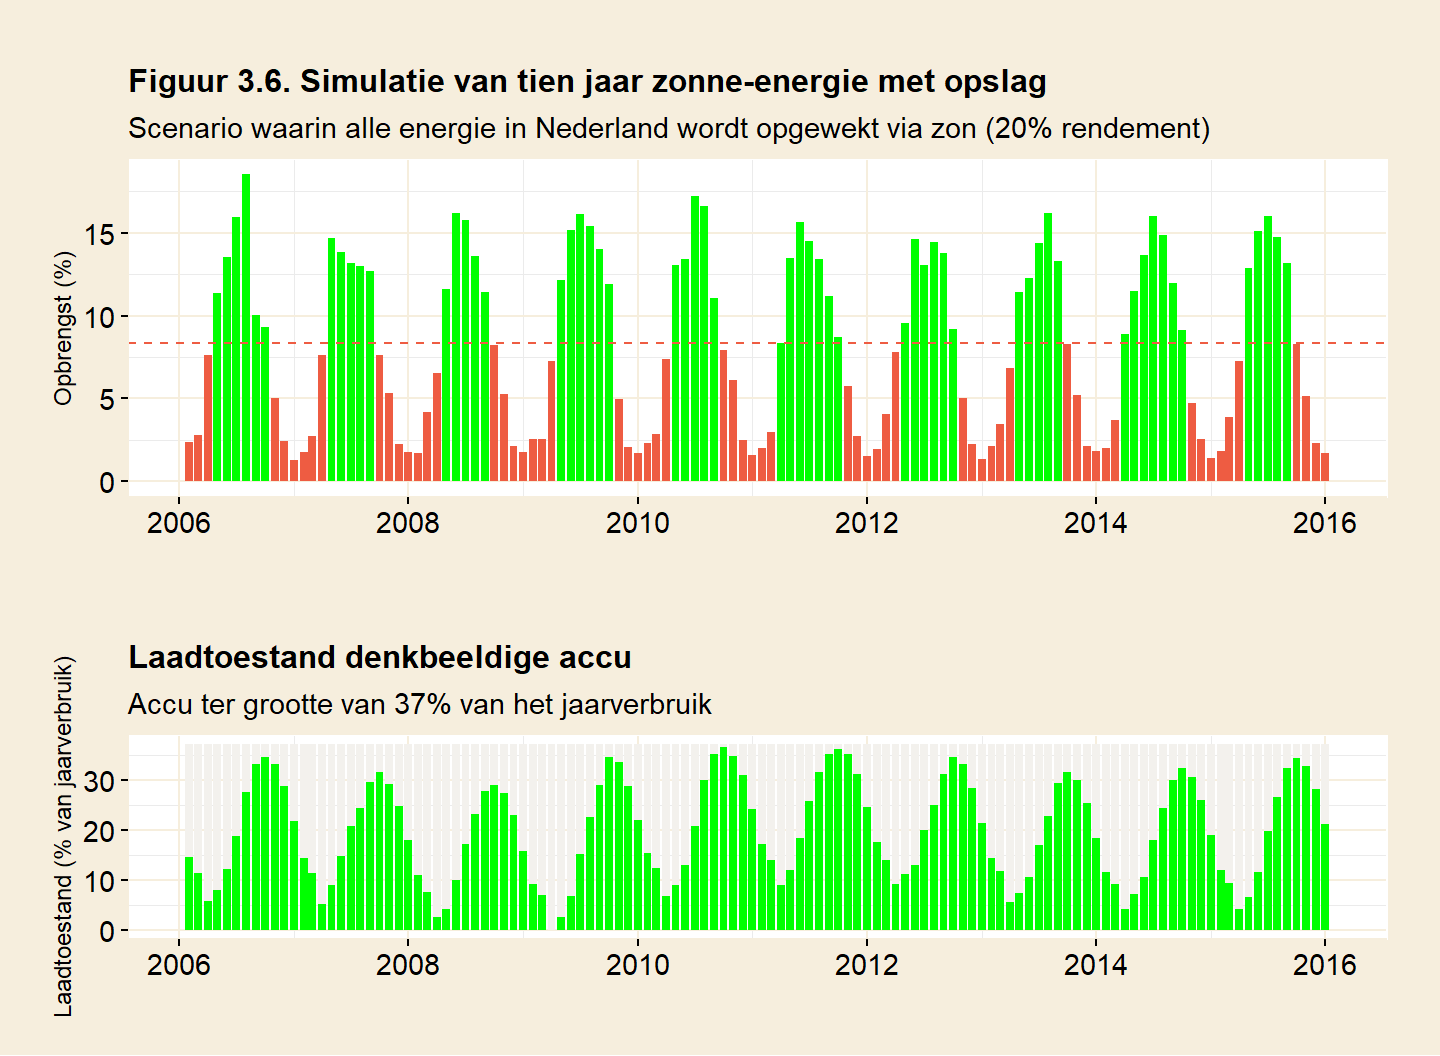
\includegraphics{04-Zonne-energie_files/figure-latex/infographic_opslag_zon-1} 

}

\end{figure}

Zowel de productie van energie in het bovenste staafdiagram als het verloop van de laadtoestand in het onderste staafdiagram vertonen grote regelmaat. Het is opvallend dat het patroon zo regelmatig is, veel regelmatiger dan voor windfluctuaties het geval was. Op maandbasis is de zoninstraling redelijk voorspelbaar (alhoewel er op dagbasis aanzienlijke variatie is).

In de onderste figuur wordt de laadtoestand weergegeven van een denkbeeldige accu. Deze denkbeeldige accu heeft een capaciteit ter grootte van 37\% van het jaarlijks Nederlands energieverbruik. Dat is precies voldoende om in deze tien jaar alle zonarme perioden op te kunnen vangen. De accu volgt het ritme van de seizoenen. In de late zomer is de accu op z'n volst en in de winter wordt de laagste stand bereikt.

Merk op dat in 2009 de laadtoestand even de 0\% raakt: de accu is nu helemaal leeg. Kleiner kan de accu dus niet zijn, anders onstaat er een energietekort. De capaciteit van de accu in deze simulatie komt overeen met 37\% van het jaarverbruik. Dat is gelijk aan ongeveer vier maanden Nederlands energiegebruik.

\hypertarget{zonne-energie-in-combinatie-met-een-hulpbron}{%
\section{Zonne-energie in combinatie met een hulpbron}\label{zonne-energie-in-combinatie-met-een-hulpbron}}

Vervolgens kan er gekeken worden naar dezelfde periode van tien jaar met dezelfde fluctuaties in opbrengst, maar ditmaal wordt er gebruik gemaakt van een hulpbron om de tekorten op te vangen. Figuur 3.7 toont weer maandtotalen, gebaseerd op tijdsvakken van 10 minuten.

\begin{figure}[!t]

{\centering \includegraphics{04-Zonne-energie_files/figure-latex/infographic_hulpbronnen-1} 

}

\end{figure}

\noindent
Het volgende beeld onstaat. Door energie bij te draaien wordt iedere maand inderdaad precies aan de energiebehoefte van Nederland voldaan. Zonne-energie (geel) en hulpbron (blauw) tezamen reiken tot de stippellijn: het verbruik van Nederland. Tevens is te zien dat er zonne-energie onbenut blijft, de grijze staven. Dat komt omdat in een scenario met enkel een hulpbron, dus zonder opslag, deze energie niet inzetbaar is. Het verlies van `nuttige' capaciteit is groot.

Wie figuur 3.6 vergelijkt met 3.7, valt het misschien op dat de overproductie in 3.7 wel groter lijkt dan het surplus in figuur 3.6. Bij de telling in figuur 3.7 wordt er onderscheid gemaakt tussen tijdsvakken met een overschot en tijdsvakken met een tekort. In figuur 3.7 is de optelling van de gele staven en de grijze staven gelijk aan de hoogte van maandstaven in figuur 3.6. Dit onderscheid ontbreekt in figuur 3.6. De extra informatie die figuur 3.7 biedt, maakt duidelijk hoeveel van de opbrengst surplus was, en hoeveel direct aan gebruikers geleverd kon worden.

Zonne-energie zorgt in totaal voor 38\% van de jaarlijkse energie en de hulpbron moet dus 62\% van de benodigde energie bijdraaien.

Ook hier geldt, net zoals werd geconstateerd bij windenergie, dat op momenten dat de zon niet schijnt, de hulpbron de totale last van de energievraag op z'n schouders krijgt. De hulpbron moet ook hier het vermogen hebben om de nationale vraag te dekken en nis daarmee op zichzelf ook dekkend voor onze energiebehoefte.

\hypertarget{opslag}{%
\chapter{Opslag}\label{opslag}}

Opslagtechnologie is belangrijk omdat het een mogelijkheid biedt de fluctuaties van zonne- en windenergie te vereffenen. Het vormt een alternatief voor een hulpbron. Als er voldoende opslag voorhanden is, kunnen (hulp)bronnen zoals fossiele energiecentrales of kerncentrales worden vermeden.
De tekorten die kunnen ontstaan bij de energieproductie met enkel zon of wind kunnen oplopen tot maanden van het Nederlands energieverbruik, zoals werd gezien bij de opbrengstberekeningen van zonne- en windenergie. Dat wil niet zeggen dat bij een combinatie van wind en zon ook zo'n grote opslag nodig zou zijn. In hoofdstuk 5 (Simulaties) gaat bekeken worden hoe groot de behoefte aan opslag is voor specifieke samenstellingen van de energiemix. Voor nu is het doel te kijken wat er voor een bepaalde opslagmethode haalbaar zou zijn.

Naast capaciteit -- het hebben van voldoende energieopslag -- is ook de snelheid waarmee omzettingen kunnen plaatsvinden van belang. Als het laden te langzaam gaat, kan er kostbare energie verloren gaan. Staat er bijvoorbeeld veel wind, dan creëert dat in potentie een groot energieoverschot. Dat overschot moet dan wel direct verwerkt kunnen worden. Neem een spaarbekken als voorbeeld. Niet alleen moet de capaciteit van het basin groot genoeg zijn, ook moet het water snel genoeg omhoog kunnen worden gepompt. Anders kan het overschot niet geheel verwerkt worden en gaat er energie verloren.

Iets dergelijks geldt voor de terugomzetting van eenmaal opslagen energie naar elektriciteit. De opslag moet genoeg vermogen hebben -- voldoende energie per tijdseenheid kunnen leveren -- om de onstane vraag te kunnen dekken. In het geval van een spaarbekken moet er niet alleen genoeg pompvermogen zijn om het bekken te vullen, maar er moet ook genoeg elektriciteit kunnen worden opgewekt om aan de maximale vraag aan te kunnen.

Een ander punt waarop gelet moet worden zijn omzettingsverliezen. Iedere vorm van opslag kent verliezen. Elektriciteit wordt bij opslag omgezet in iets anders: een chemische reactie in het geval van een accu, de potentiële energie van water dat omhoog werd gepompt in het geval van een spaarbekken, etc. Bij al deze omzettingen vinden verliezen plaats. Als een opslagmethode grote omzettingsverliezen kent, zal dit verlies moeten worden gecompenseerd door meer energie op te wekken.

\hypertarget{spaarbekkens}{%
\section{Spaarbekkens}\label{spaarbekkens}}

Een reden om spaarbekkens als energie-opslagmethode te overwegen, is dat het qua capaciteit wereldwijd de meest gebruikte vorm van energie-opslag is. Spaarbekkens maken 95\% van de wereldwijde opslagcapaciteit uit. Dat zal niet voor niets zijn. Wereldwijd is er volgens wikipedia ruim 1.6 TWh beschikbaar (\href{https://en.wikipedia.org/wiki/Pumped-storage_hydroelectricity}{zie wikipedia/ pumped-storage hydroelectricity}). Dat klinkt veel, maar in termen van nationaal energieverbruik (706 TWh in 2019) is dat slechts 20 uur (365 dagen * 24 uur * 1.6 TWh / 706 Twh = 20 uur). Gemiddeld, vindt wikipedia, is een spaarbekken in een uur of tien te vullen.

Uit dit rekenvoorbeeld blijkt dat de gezochte opslagcapaciteit groot is. Nederland verbruikt veel energie: zelfs het opslaan van een dag van ons energieverbruik vergt al meer dan er mondiaal in spaarbekkens beschikbaar is. Het gaat om massa-opslag van energie op een schaal die nog niet eerder is gerealiseerd.

Dat geeft de uitdaging aan, maar er kan geprobeerd worden de huidige capaciteit aan spaarbekkens in de toekomst uit te breiden. Om daar een inschatting van te maken -- hoe energie-opslag in spaarbekkens schaalt -- is wat meer achtergrond nodig. Aan spaarbekkens valt makkelijk zelf te rekenen, zodat er zelf een inschatting te maken is met behulp van basisprincipes.

Bij een spaarbekken wordt een hoog gelegen basin verbonden met een lager gelegen basin. Het hoger gelegen basin wordt gebruikt voor opslag van energie. Tussen de basins bevindt zich een pompcentrale. Als er een overschot van elektriciteit is, kan de pompcentrale worden gebruikt om water van het laaggelegen basin naar het hooggelegen basin te pompen. Dezelfde pompcentrale kan worden gebruikt om energie terug op te wekken: de waterdruk zet nu de turbine in beweging en daarmee wordt stroom opgewekt.

Het rendement van deze opslagmethode ligt rond de 75\%; er gaat dus zo'n 25\% van de energie verloren. Dat is redelijk efficiënt. Gunstig is ook dat energie probleemloos voor lange tijd kan worden opgeslagen: het water blijft gewoon waar het is. Ook het onderhoud is miniem: een spaarbekken en pompcentrale kunnen vele tientallen jaren mee zonder dat er groot onderhoud gedaan hoeft te worden.

De hoeveelheid energie, in Joule, die een spaarbekken kan opslaan is afhankelijk van hoeveel al dat water weegt (\(m\)), de hoogte (\(h\)) van het verval van het spaarbekken en de valversnelling (\(g\)): \(E = m \; g \; h\).

In de Nederlandse context denk men al snel aan het IJsselmeer als groot water dat misschien gebruikt zou kunnen worden voor energie-opslag. Stel, als gedachtenexperiment, dat het IJsselmeer en het Markermeer tezamen zou worden gebruikt als spaarbekken door de dijk erom met twee meter te verhogen.

Het verval van dit spaarbekken is twee meter, als het bekken helemaal vol zit. Het gemiddelde verval van dit enkele spaarbekken is de helft daarvan, één meter. Het IJsselmeer en Markermeer zijn bij elkaar 1800 km\textsuperscript{2} groot. Een kubieke meter water weegt 1000 kg, dus dit oppervlakte weegt bij één meter diepte \(1800\) miljard kg. De opgeslagen energie die dit meer vertegenwoordigt, is daarmee gelijk aan \(1800\) miljard kg \(\times\) 10 m/s = \(18000\) GJ. Om dat in perspectief te zetten: Nederland gebruikt een continue vermogen van ongeveer 81 GJ per seconde, dus dit spaarbekken is in staat om 4 minuten van ons energieverbuik op te slaan.

Dat is teleurstellend, want de massa-opslag waarna we op zoek zijn zit meer in de orde van grootte van dagen tot weken, misschien zelfs maanden. Beide meren vertegenwoordigen al een substantieel deel van ons binnenwater, dus heel veel meer oppervlakte is niet realiseerbaar. Als we een \emph{dag} van ons nationaal energieverbruik zouden willen opslaan, dan zou de dijk 774 meter hoog moeten zijn.

Zwaartekracht is een relatief zwakke kracht en dat betekent dat het hoogteverschil de sleutel is tot effectieve energieopslag in een spaarbekken. Hoogteverschil is iets dat in Nederland niet ruim voorhanden is, dus hiervoor zal naar het buitenland moeten worden uitgeweken. Men zou bijvoorbeeld kunnen denken aan de Alpen, of aan Noorwegen.

Om met de laatste te beginnen, de Noorse kust kent vele fjorden. Het omringende landschap is hoog, dus daar kan gebruik van worden gemaakt. Een fjord grenst aan zee, wat het vullen van een eventueel spaarbekken zal vergemakkelijken.

Het grootste fjord van Noorwegen, het Sognefjord, is grofweg 120 km lang en 5 km breed. Het omringende landschap reikt tot een kilometer hoog. Stel dat het fjord zodanig wordt ingedamd dan het waterniveau met een halve kilometer kan worden verhoogd.

Hoeveel potentiële energie kan er in dit fjord worden opgeslagen? De berekening is in principe dezelfde als net voor het IJsselmeer is gedaan. De massa van het water in het afgedamde fjord is gelijk aan 120.000 m \(\times\) 5.000 m \(\times\) 500 m \(\times\) 1.000 kg = 300000 miljard kg. Bij een verval van 250 meter, de helft van de hoogte van de bak, betekent dat een energieopslag van 75 miljoen GJ.

Dat zijn enorme getallen, maar afgemeten tegen het energieverbruik van Nederland is dat nog steeds relatief. Bij een continue vermogen van 81 GW, is deze opslag equivalent aan 75 miljoen GJ / 81 GW / 3600 seconden / 24 uur = 10.8 dagen nationaal energieverbuik. Een blik op de kaart van Noorwegen leert dat de hoeveelheid fjorden van grote omvang eindig is. Misschien dat er nog een handvol te vinden is? Moeten die allemaal worden afgedamd? Als dat al lukt, zouden er nog andere landen in Europa zijn die de Noren zouden vragen om energieopslag, als zij ook fluctuerende bronnen zouden hebben?

Deze gedachtenexperimenten geven een idee van de grootte van de opslag die met spaarbekkens te realiseren is. De berekening kijkt alleen naar capaciteit, maar er zijn nog vele andere zaken die ook zouden moeten worden opgelost. Bijvoorbeeld: kan er bij terugwinning van de energie wel voldoende vermogen worden opgewekt om aan het tekort te voldoen? Om Nederland 10 dagen lang van energie te voorzien, moet het fjord ook in die tijd geleegd kunnen worden. Dat betekent meer pijpen en pompcentrales. Is dat haalbaar? En hoe enthousiast zouden de Noren zelf over dit plan zijn?

Er is natuurlijk nog een ander gebergte in Europa: de Alpen. Helaas leent de ligging van de alpen zich niet goed voor massale energieopslag. De Alpen liggen ver van zee. Een spaarbekken heeft water nodig. Het lage reservoir van waaruit het water naar boven wordt gepompt, moet zich op zo kort mogelijke afstand van het hoge reservoir bevinden. Hoe langer de afstand, des te meer wrijving moet worden overwonnen en dat geeft energieverlies. En men zal zeewater nodig hebben. De benodigde hoeveelheid water is in de Alpen eenvoudigweg niet voorhanden. Zelfs het meer van Genève is, hoewel aanzienlijk dieper, met een oppervlakte van 584 km\textsuperscript{2} klein t.o.v. ons eigen IJsselmeer met 1100 km\textsuperscript{2}.

\hypertarget{accus}{%
\section{Accu's}\label{accus}}

Accu's vormen een andere manier om energie op te slaan. Er zijn vele \href{https://nl.wikipedia.org/wiki/Oplaadbare_batterij}{typen accu's} met eigenschappen die onderling van elkaar verschillen. Om te beginnen de energiedichtheid, hoeveel capaciteit men voor een bepaald gewicht aan accu's kan realiseren. De efficiëntie (\emph{roundtrip efficiency} of retourefficiëntie) is een ander belangrijk aspect. Dat geeft aan hoe groot de verliezen zijn bij opslag en weer teruggave van energie. Daarnaast zijn er verschillen in de laad- en ontlaadtijd van een accu. Al deze punten zijn van belang voor de toepassing van accu's als massa-opslagmedium.

Wat bijzonder is aan accu's, is dat de snelheid waarmee energie wordt geladen en ontladen van grote invloed kan zijn op zowel de capaciteit als de levensduur van de accu. Het kan zo zijn dat men op papier genoeg capaciteit heeft om aan een bepaalde opslagbehoefte te voldoen, maar dat de snelheid waarmee geladen of ontladen wordt de capaciteit verkleint. Dat betekent dat er meer accu's nodig zijn en de installatie duurder wordt.

\hypertarget{lithium}{%
\subsection{Lithium}\label{lithium}}

Van alle accutypen hebben \href{https://en.wikipedia.org/wiki/Lithium-ion_battery}{Lithium-ion-accu's} de hoogste energiedichtheid en combineren dat met een korte laad- en ontlaadtijd. Dat betekent dat er voor het gewicht van een accu veel energie beschikbaar is en dit type wordt dan ook gebruikt in elektrische auto's. Het wordt ook gebruikt als oplossing voor massa-opslag van elektriciteit.

Lithiumaccu's hebben een \href{https://en.wikipedia.org/wiki/Comparison_of_commercial_battery_types\#Rechargeable_characteristics}{retourefficiëntie van 90\%}. Er gaat dus weinig energie verloren in het proces van opslag naar teruglevering van energie. De hoge efficiëntie betekent dat er slechts weinig overcapaciteit gerealiseerd hoeft te worden om de verliezen te compenseren.

Om de levensduur te vergroten is het beter om lithium-ion accu's niet verder te ontladen dan tot \href{https://nl.wikipedia.org/wiki/Lithium-ion-accu}{30\% van de capaciteit en niet meer te laden dan tot 80\% van de capaciteit}. Als men zich hieraan wil houden, dan moeten er dus meer accu's worden aangeschaft voor een bepaalde gewenste capaciteit. Het alternatief om wel volledig te laden en ontladen, maar dan moeten de accu's sneller worden vervangen. Vervanging probeert men in de praktijk zoveel mogelijk te voorkomen, omdat lithium-ion accu's duur zijn. Dat betekent niet dat een accu niet snel kán ontladen. Een lithium-accu kan bijvoorbeeld in een uur worden ontladen en daarmee een hoog vermogen genereren. In dat geval is het vermogen gelijk aan z'n capaciteit: als de accu 1 kWh bevat, kan deze een uur lang een vermogen leveren van een kilowatt. De keerzijde is dan wel snellere vervanging.

\hypertarget{lood}{%
\subsection{Lood}\label{lood}}

\href{https://nl.wikipedia.org/wiki/Loodaccu}{Loodaccu's} zijn het oudste type accu, commercieel beschikbaar sinds 1881. Ze zijn relatief goedkoop en hebben een retourefficiëntie van rond de 85\%. Net als bij lithium-ion accu's is dat efficiënt.

Een nadeel is dat de ontlading eigenlijk niet meer dan 50\% mag bedragen, als men de levensduur niet teveel wil bekorten. Dat betekent dat men twee keer meer accu's moet plaatsen dan de capaciteit aangeeft, om die capaciteit ook daadwerkelijk te realiseren.

Snel ontladen van een loodaccu beperkt de capaciteit drastisch: de aangegeven (nominale) capaciteit wordt berekend over een afnameperiode van 10 uur. Bij ontlading in minder dan een uur blijft daar slechts 50\% van over (zie vorig wikipedia lemma). De beperkte diepte van de ontlading en de kleinere capaciteit bij snelle ontlading betekenen in feite dat men bij loodaccu's een flinke overcapaciteit moet hanteren wil men snel vermogen kunnen afgeven.

\hypertarget{grondstoffen}{%
\subsection{Grondstoffen}\label{grondstoffen}}

Als accu's gebruikt gaan worden voor massa-opslag, dan zullen er veel van nodig zijn. Het is dus relevant de vraag te stellen of er genoeg grondstoffen voorhanden zijn.

De mondiale \href{https://en.wikipedia.org/wiki/Lithium\#Reserves}{reserves van lithium} zijn volgens wikipedia 86 miljard kg groot. Een accu gebruikt \href{https://publications.lib.chalmers.se/records/fulltext/230991/local_230991.pdf}{0,16 kg lithium per kWh} volgens een onderzoek van Chalmers university. Daarmee kan geschat worden hoeveel kWh er aan lithium-accu's in totaal gemaakt kan worden: \(86 \times 10^9 / 0.16 = 5.4 \times 10^{11}\) kWh \(= 540\) TWh. Met de wereldwijd bekende reserves zou dus een hoeveelheid accu's kunnen worden gemaakt met een capaciteit ter grootte van ongeveer driekwart het jaarlijks Nederlands energieverbruik, als wordt gerekend met de al eerder gebruikte 706 TWh voor 2019.

Deze reserve zou voldoende zijn voor Nederland alleen, maar mondiaal gezien is het weinig. Ook andere landen zullen aanspraak willen maken op de voorraad lithium, zeker als accu's een effectieve opslagmethode blijken te zijn. Als de hoeveelheid lithium eerlijk over de wereld verdeeld zou worden, dan blijft er voor Nederland minder dan een dag aan opslagcapaciteit over (17 miljoen Nederlanders gedeeld door 7 miljard aardbewoners maal driekwart jaar is ongeveer tweederde dag).

Hoe zit dit met loodaccu's? De \href{https://www.statista.com/statistics/1156095/global-lead-reserves/}{wereldwijde loodreserves} bedragen 88 miljard kg, volgens statista.com. Zestig procent van het gewicht van een \href{https://en.wikipedia.org/wiki/Lead\%E2\%80\%93acid_battery}{loodzuuraccu} bestaat uit lood. De energiedichtheid is volgens wikipedia 40 Wh/kg. Zestig procent van het gewicht van een accu is lood. Gerekend naar het gewicht van lood is dat 40 / 0.6 = 67 Wh/kg. Per kWh gebruikt een loodaccu daarmee 1 / 0.067 = 15 kg lood.

Daarmee kan geschat worden hoeveel kWh er aan loodaccu's in totaal gemaakt kan worden: \(88 \times 10^9 / 15 = 5.7 \times 10^{9}\) kWh \(= 5.7\) TWh. Dat komt neer op ongeveer 3 dagen Nederlands energieverbruik. Als we het lood ook eerlijk over de wereld zouden verdelen, dan blijft er niet veel capaciteit over.

\hypertarget{waterstof}{%
\section{Waterstof}\label{waterstof}}

Waterstof is aantrekkelijk als energiedrager omdat bij de verbranding ervan geen CO\textsubscript{2} wordt gevormd. Het laat enkel water achter. Er wordt veel van verwacht, bijvoorbeeld door de Europese Unie, die het een belangrijk onderdeel heeft gemaakt van de energietransitie. Men ziet het gebruikt worden als brandstof en als een manier van massa-opslag om de fluctuaties van niet-continue energiebronnen op te vangen.

Waterstof heeft een hoge \href{https://en.wikipedia.org/wiki/Energy_density}{energiedichtheid} per gewicht. Per kilogram levert het 3 keer meer energie dan benzine. Waterstofgas heeft echter geen grote dichtheid, waardoor het per volume juist minder energie in zich draagt dan benzine. Per liter is de energiedichtheid van waterstof slechts \(\frac{1}{3000}\) van benzine. Deze lage energiedichtheid valt te verbeteren door het gas te comprimeren. Bij 690 bar bevat het gas \(\frac{1}{8}\) van de energie van een vergelijkbare hoeveelheid benzine. \href{https://en.wikipedia.org/wiki/Liquid_hydrogen}{Vloeibaar waterstof} heeft de hoogste energiedichtheid, maar bezine blijft ook dan nog een factor 4 energiedichter. Om waterstof vloeibaar te maken, moet het gekoeld worden tot -253° C.

In tegenstelling tot fossiele brandstoffen is er geen natuurlijke bron van waterstof. Waterstof moet worden gemaakt. De elektriciteit uit zonne- en windenergie kan hiervoor worden ingezet. Dat kan via elektrolyse, bijvoorbeeld met behulp van een \href{https://en.wikipedia.org/wiki/Polymer_electrolyte_membrane_electrolysis}{PEM-elektrolyser}. Een PEM-elektrolyser kan elektriciteit in waterstof omzetten met een efficiëntie van zo'n \href{https://en.wikipedia.org/wiki/Polymer_electrolyte_membrane_electrolysis\#PEM_Efficiency}{80\%}.

Voor \href{https://en.wikipedia.org/wiki/Hydrogen_storage\#Underground_hydrogen_storage}{massaopslag van energie met behulp van waterstof} zijn door de lage energiedichtheid grote ruimten nodig, zelfs als het wordt gecomprimeerd. Opslagtanks zijn niet toereikend. Men denkt aan opslag in zoutkoepels en oude gasvelden, waarbij de waterstof wordt gecomprimeerd tot zo'n 200 bar. Het comprimeren kost het equivalent van 2\% van de opgeslagen hoeveelheid waterstof aan energie.

Om energie weer terug te winnen, wordt de waterstof verbrand. Dat kan met behulp van een \href{https://en.wikipedia.org/wiki/Fuel_cell}{brandstofcel}, of via verbranding in een \href{https://www.ipieca.org/resources/energy-efficiency-solutions/power-and-heat-generation/combined-cycle-gas-turbines/}{gasturbine}. Daarmee wordt er dan weer elektriciteit geproduceerd. De efficiëntie van beide methoden ligt rond de 50\%.

\hypertarget{efficiuxebntie}{%
\subsection{Efficiëntie}\label{efficiuxebntie}}

De efficiëntie van de omzettingen is belangrijk wanneer waterstof als energieopslag wordt gebruikt. Hoe meer energie er verloren gaat, hoe meer er eerst geproduceerd moet worden. De \emph{roundtrip efficiency} (retourefficiëntie) van energie-opslag met behulp van waterstof is dus ongeveer 80\% \(\times\) 50\% = 40\%. Nadat de elektrolyser waterstof heeft geproduceerd, resteert 80\% van de ingezette energie. Na verbranding in de gasturbine voor de terugopwekking van stroom blijft daar de helft van over. Uiteindelijk resteert er 40\% van de oorspronkelijke ingezette energie. Anders gezegd gaat er dus 60\% van de energie bij opslag verloren. Dat betekent dat er twee en een half keer meer energie geproduceerd moet worden dan er uiteindelijk uit de opslag gebruikt kan worden. Waterstof is dus een inefficiënte manier van energie-opslag. Vergelijk dit bijvoorbeeld met een accu die een efficiëntie van 90\% kan halen. Om het verlies van de accu te compenseren, hoeft er slechts 11\% overcapaciteit te worden gerealiseerd.

\hypertarget{infrastructuur}{%
\subsection{Infrastructuur}\label{infrastructuur}}

Om waterstof te kunnen gebruiken als energie-opslag, is er aanzienlijk meer infrastructuur nodig dan het geval is voor accu's. Eenvoudig gezegd: om accu's te laden, is het voldoende om stroom op de polen te zetten, en voor stroomproductie hoeft men alleen de polen te verbinden met een gebruiker. Qua infrastructuur is er eigenlijk niet veel meer nodig dan de accu zelf en wat bedrading. Bij waterstof ligt dat gecompliceerder.

Voor de productie van waterstof heeft men waterstoffabrieken nodig, die met behulp van elektrolyse waterstof kunnen produceren. De principes en de technologie hiervoor zijn bekend, maar in de praktijk gebeurt dit alleen nog op beperkte schaal. In 2020 werd de tot dan toe \href{https://allesoverwaterstof.nl/s-werelds-grootste-pem-elektrolyser-in-gebruik-genomen/}{grootste PEM elektrolyser} ter wereld in gebruik genomen. De fabriek staat in Canada en heeft een vermogen van 20 megawatt (MW). Eenzelfde vermogen is gepland voor een \href{https://www.gasunienewenergy.nl/projecten/djewels}{proeffabriek in Delfzijl}, die later opgeschaald moet worden naar 60 MW.

Hoe verhoudt het productievermogen van deze fabrieken zich tot het Nederlandse energieverbruik? Nederland verbruikte in 2019 gemiddeld 81 GW aan energie. Waterstof kan worden gemaakt op het moment dat variabele bronnen, zoals zon en wind, meer produceren dan we nodig hebben. Zoals bleek uit hoofdstukken 2 en 3 kan deze energieproductie het dubbele zijn van wat er op dat moment nodig is. Om een dergelijke overproductie te kunnen omzetten in waterstof zijn daar dan 81 GW / 20MW = 4050 waterstoffabrieken van het type Delfzijl voor nodig. Er moet immers genoeg vermogen zijn om de overcapaciteit te kunnen verwerken als deze zich voordoet. Afgezet tegen de energiebehoeften van Nederland lijkt er met de huidige stand van zaken een aanzienlijke infrastructuur voor de productie van waterstof nodig.

Het voorgaande betrof de productiekant van waterstof. Vervolgens moet de waterstof worden opgeslagen. Dat lijkt te kunnen, in volumes die bruikbaar zijn voor massaopslag, in oude gasvelden. Men denkt dat Nederland er daar voldoende van heeft.

Uiteindelijk moet de energie worden teruggewonnen, en daar is opnieuw aparte infrastructuur voor nodig. Verbranden kan onder andere in aangepaste gascentrales. Hoe verhoudt deze infrastructuur zich met de Nederlandse situatie? Op het moment dat wind en zon geen energie kunnen leveren, is er 81 GW aan vermogen nodig. De grootste gascentrale in Nederland, de \href{https://nl.wikipedia.org/wiki/Lijst_van_elektriciteitscentrales_in_Nederland}{Clauscentrale} in Maasbracht (Maasbracht-C), levert 1,3 GW. Daarvan zouden er dus 81 GW / 1,3 GW = 62 centrales nodig zijn.

Al met al is duidelijk dat waterstof als opslagmethode in de context van het Nederlands energieverbruik een aanzienlijke infrastructuur vergt. Er zijn waterstoffabrieken nodig, oude gasvelden inclusief de benodigde infrastructuur voor transport en compressie, en uiteindelijk elektriciteitscentrales waarin de waterstof weer verbrand kan worden.

\hypertarget{de-energiemix}{%
\chapter{De energiemix}\label{de-energiemix}}

Het voorbereidende werk is achter de rug, nu is het hoog tijd een energiemix te gaan samenstellen. Het doel van dit hoofdstuk is te onderzoeken hoe betrouwbare energielevering mogelijk wordt met duurzame bronnen. Variabele energiebronnen vertonen uitval, dat is de aard van de bron. De uitval moet op een of andere manier gecompenseerd worden. Continue energiebronnen, zoals kolen- en gascentrales, of kerncentrales, kennen deze problematiek niet. Een continue energiebron geeft een betrouwbare energieproductie, zoals we nu zijn gewend op basis van fossiele brandstoffen. Niet-continue bronnen staan in de simulaties centraal, juist omdat die niet in staat zijn permanent energie te leveren. Verdere infrastructuur die wordt gebruikt is daar in de simulaties secundair aan en wordt gebruikt om tekorten te vereffenen.

De bedoeling is niet om de perfecte energiemix te vinden, maar om inzicht te krijgen in de werking daarvan. Inzicht krijgen van het effect van een bepaalde mix van energiebronnen is niet meer op de achterkant van een envelop te doen, zoals het bijvoorbeeld voor spaarbekkens nog wel aardig lukt. De onvoorspelbaarheid van de opbrengst uit zonne- en windenergie is daar een belangrijke oorzaak van. Vooral in het geval van windenergie, waar windsnelheidsverschillen een grote impact hebben op de opbrengst, is een schatting lastig te maken als er niet in detail gekeken wordt. Datzelfde geldt voor het verloop van de pieken en dalen in de opbrengst. Tekorten kunnen zich in de loop van de tijd opstapelen. Het precieze verloop van overschot en tekort is bepalend voor de hoeveelheid opslag, hulpenergiecentrales en andere infrastructuur die nodig is.

Om toch de gevolgen te kunnen bekijken van verschillende samenstellingen van een energiemix, wordt hier gebruik gemaakt van een rekenmodel dat opbrengst en tekort in tijdsstappen van tien minuten berekent. Dat geeft het detail om voor een bepaalde samenstelling van een energiemix te zien wat de gevolgen zijn van de gemaakte keuzes.

Hoe het model werkt, wordt hieronder eerst beschreven. Vervolgens worden er in de rest van het hoofdstuk een aantal vragen uitgewerkt. Iedere vraag behandelt een andere invulling van de energiemix. De simulaties schetsen de gevolgen, volgens het model, van de keuze voor een bepaalde inrichting van de energiemix. Er zijn daarvoor veel scenario's mogelijk. Hier is gekozen voor een aantal varianten die de wisselwerking tussen de verschillende ingrediënten van een energiemix het beste duidelijk maken en tevens iets zeggen over de schaal van de onderneming.

\hypertarget{het-model}{%
\section{Het model}\label{het-model}}

Een energiemix bestaat in het model uit niet-continue bronnen (zon en wind), een vorm van opslag (bijvoorbeeld spaarbekkens, accu's of waterstof) en een continue bron (zoals `schone' gascentrales of kerncentrales).

Het model gaat ervan uit dat Nederland niet op enig moment zonder energie mag komen te zitten. Het is zodanig ingericht dat eventuele tekorten altijd direct worden vereffend. Zon en wind worden beschouwd als primaire energieleveranciers. Eventuele opslag of hulpbronnen worden pas aangesproken op het moment dat wind en zon niet meer in staat zijn de vraag te dekken.

De simulaties nemen zoals eerder het nationale energieverbruik van 2019 als uitgangspunt (706 TWh). Er wordt aangenomen dat de nationale energievraag constant is. Nederland verbruikt dan continu zo'n 81 GW aan energie. Het \emph{vermogen} om Nederland aan de praat te houden is 81 GW, de \emph{hoeveelheid energie} die in een jaar wordt verbruikt is 706 TWh.

De simulaties gaan uit van een constant energieverbruik en dat is natuurlijk een benadering van de werkelijkheid, maar het is zeker niet het slechtste scenario. Stel dat de vraag niet constant is, maar fluctueert. Soms zal het zo zijn dat een windarme periode inderdaad samenvalt met weinig vraag. Er zijn echter ook momenten dat de vraag bovengemiddeld is, hetgeen een groter vermogen vraagt van de energiebron dan bij constante vraag. Het vermogen, en daarmee het aantal windmolens of centrales dat er moet staan, of het aantal accu's dat wordt gebruikt, neemt toe.

De uitkomsten van het model bieden inzicht in de opbrengstfluctuaties van een bepaalde energiemix en de bijbehorende infrastructuur die nodig is om de vraag sluitend te krijgen. De boekhouding dient daarbij te kloppen. Het model beperkt zich tot de Nederland. Dat is ingegeven door bekendheid met de Nederlandse situatie en door de uitstekende gegevens die voorhanden zijn om opbrengst uit zon en wind fijnmazig te berekenen. Om de balans kloppend te houden wordt er geen energie van buiten gebruikt. Nederland moet zichzelf in het model kunnen redden.

Dit laatste lijkt vreemd. Nederland is verbonden met Europa. Het kan toch zeker geen probleem zijn om energie uit het buitenland te betrekken als dat zo uitkomt? Het energienet is immers met elkaar verbonden. Het probleem daarmee is dat deze bronnen niet in het model verantwoord worden. Het model zou dan moeten worden uitgebreid en heel Europa moeten bevatten. Men weet anders niet of het waaide of de zon scheen bij de buren, of er overcapaciteit voor ons beschikbaar was, of de energie wel duurzaam werd opgewekt en of men bereid was voor ons te investeren in energiecapaciteit. Niet verantwoorde `import' van energie maakt een model onbetrouwbaar.

\bigskip\noindent
Figuur 5.1 toont de energiestromen tussen de verschillende onderdelen in het model. Iedere tien minuten wordt het schema doorlopen. Dat begint met het berekenen van de opbrengst uit zon en wind. Er wordt wederom gebruik gemaakt van de gegevenssets van het KNMI aan de hand waarvan de opbrengsten van wind- en zonne-energie per tien minuten worden berekend.

\begin{figure}[H]

{\centering 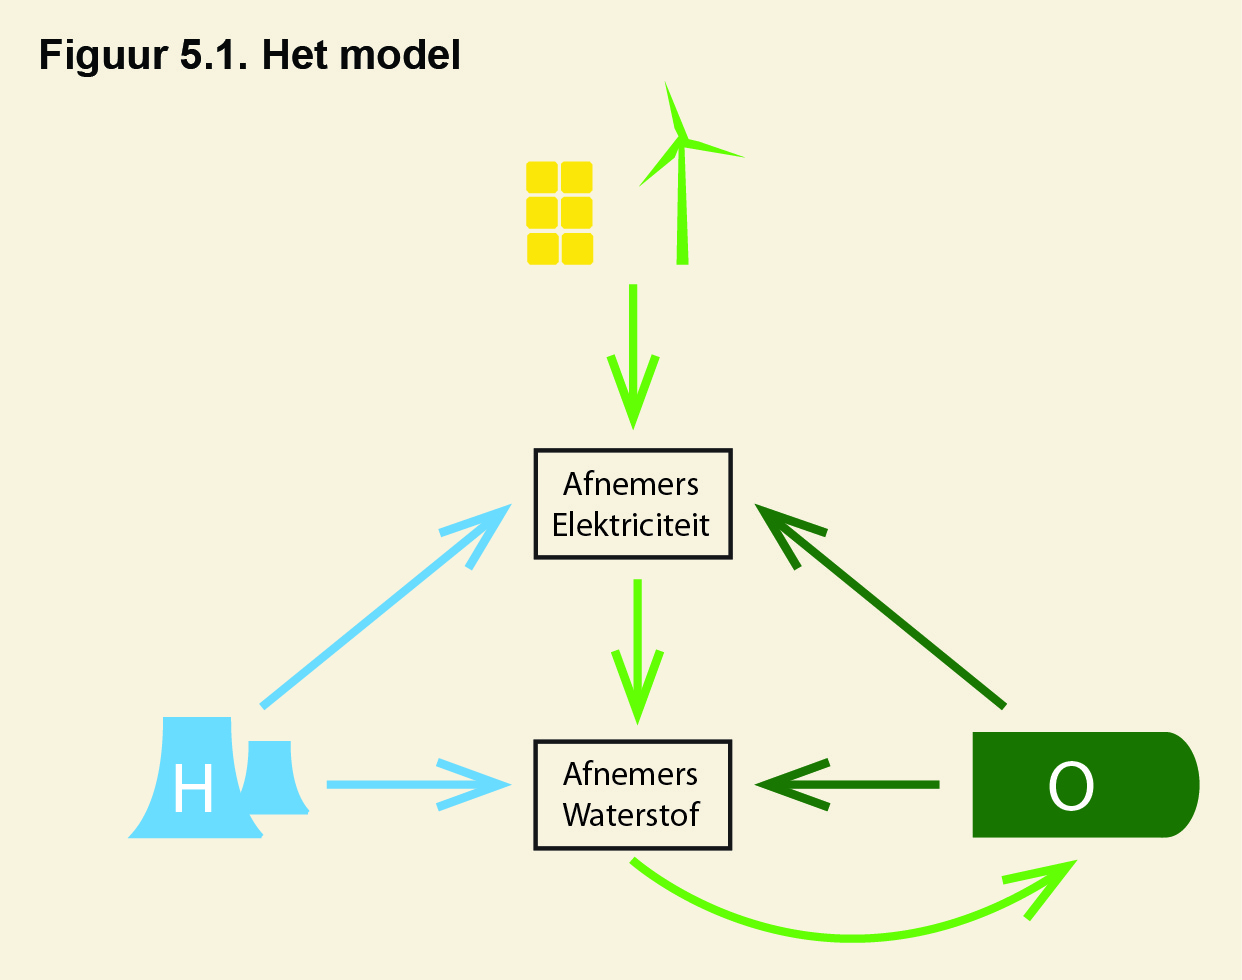
\includegraphics[width=0.7\linewidth,height=0.7\textheight]{Model energiemix eenvoudig} 

}

\end{figure}

De energievraag wordt gesplitst in een vraag naar elektriciteit en een vraag naar waterstof. Deze verhouding wordt vooraf vastgesteld (bijvoorbeeld 20\% van de vraag wordt verbruikt als waterstof en 80\% als elektriciteit). Met de opbrengst uit zon en wind wordt eerst geprobeerd aan de elektriciteitsvraag te voldoen. Lukt dat niet, dan wordt energie uit de opslag (O) betrokken. Biedt de opslag ook geen uitkomst, dan neemt het model aan dat er moet worden bijgedraaid door de hulpbron (H). De hulpbron blijft staande bij en is altijd in staat om tekorten op te vangen. Op deze manier zijn vraag en aanbod in balans te krijgen.

Nadat er aan de elektriciteitsvraag is voldaan, komen de afnemers van waterstof aan bod. Met de resterende energie uit de vorige stap wordt waterstof geproduceerd. Mocht er onvoldoende energie zijn overgebleven, dan wordt het energietekort weer aangevuld via opslag of hulpbron.

Bij sommige stappen in het model treden er verliezen op. Dat is bijvoorbeeld zo bij de productie van waterstof uit elektriciteit. Daarbij wordt uitgegaan van een efficiëntieverlies van 20\%. Dit gebeurt bij de productie van waterstof uit elektriciteit uit zonne- of windenergie, of uit elektriciteit die afkomstig is van een hulpbron. Bij de productie van elektriciteit uit waterstof wordt er met een verlies van 50\% gerekend. Dit is het geval als er uit de waterstofopslag elektriciteit moet worden geproduceerd. Bij gebruik van lithium-accu's als opslag wordt met 10\% verlies gerekend. Levering van elektriciteit door zon, wind of hulpbron aan afnemers van elektriciteit verloopt in het model zonder verlies. Hetzelfde geldt voor compressie van de waterstof voor opslag. Ook transport en levering van waterstof verloopt zonder verliezen.

Alle simulaties gaan ervan uit dat de zonnecellen een efficiëntie hebben van 20\%. Windmolens staan opgesteld in een fictief windpark op een onderlinge afstand van 7 wiekdiameters. De windmolens in het park hebben een efficiëntie van 60\%. Om de opbrengst van de molens te berekenen wordt de opbrengstkarakteristiek van de Enercon-126 gebruikt.

\hypertarget{een-dag-energieopwekking}{%
\section{Een dag energieopwekking}\label{een-dag-energieopwekking}}

Figuur 5.2 laat ter illustratie een dag energieopwekking zien met behulp van wind, zon, een hulpbron en opslag. De figuur werd samengesteld aan de hand van windsnelheid en instralingswaarden van het KNMI die voor tijdsvakken van tien minuten beschikbaar zijn. De figuur laat zien hoeveel energie een bepaalde bron op een bepaald moment opwekte. Daarnaast wordt het verloop van de opslag getoond zodat het samenspel tussen fluctuerende bron, opslag en hulpbron zichtbaar wordt.

\begin{figure}

{\centering 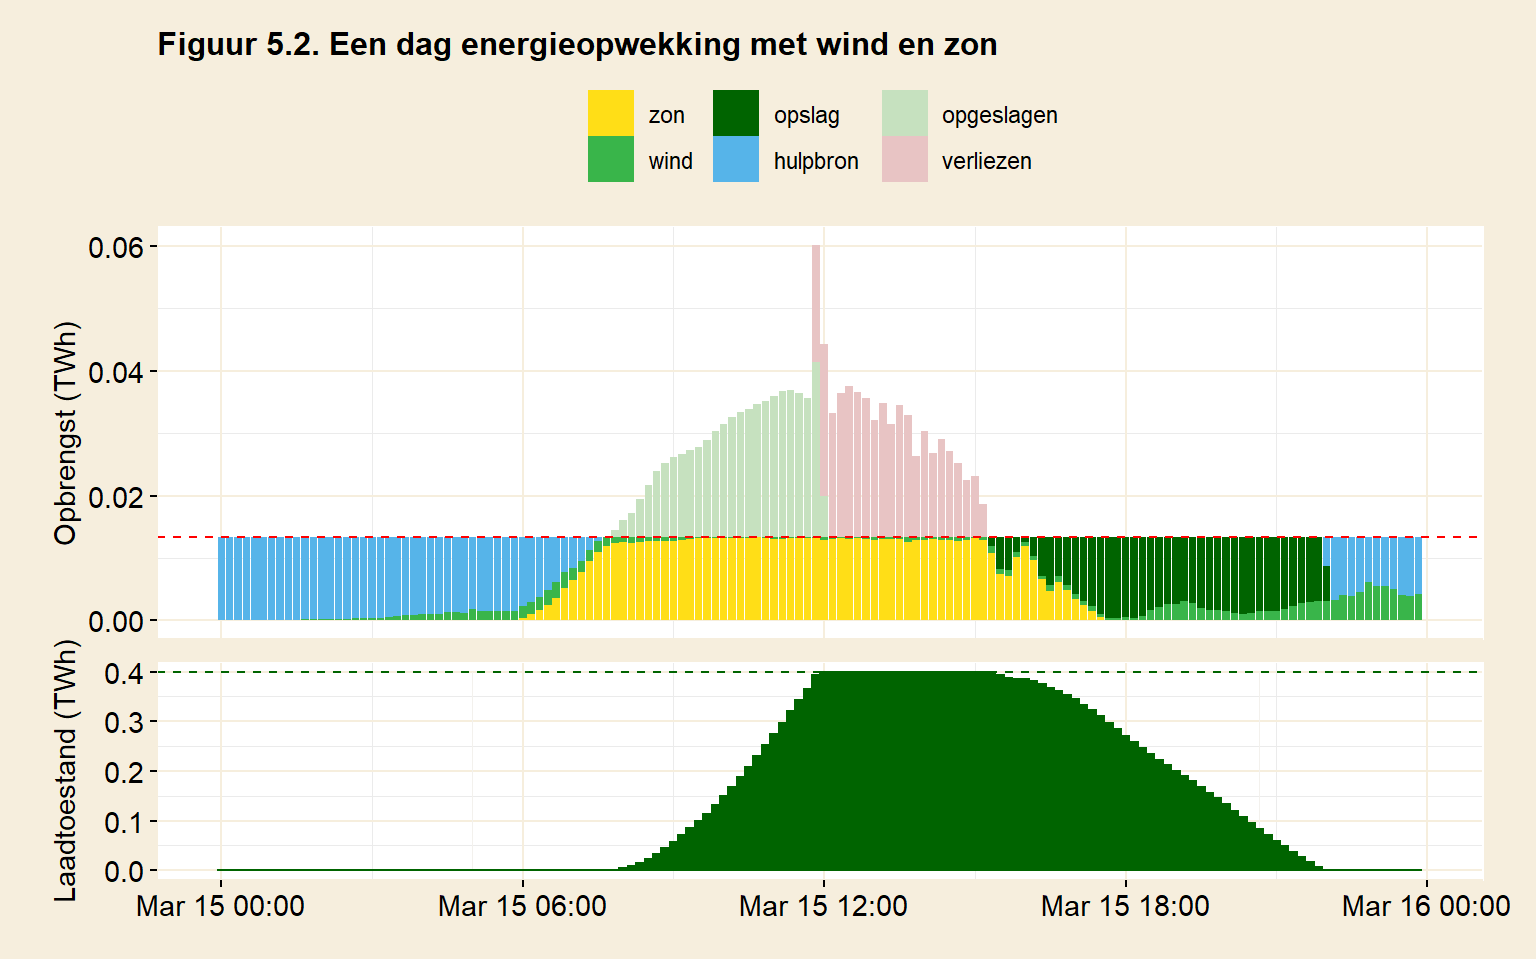
\includegraphics{06-Simulaties_files/figure-latex/dag-1} 

}

\end{figure}

De vroege ochtend begint windstil en uiteraard zonloos. Aan het begin van de dag is de opslag leeg. Dat is te zien aan de laadtoestand, het onderste gedeelte van de figuur. De hulpbron zorgt voor energie, precies genoeg om aan de vraag te voldoen (de rode stippellijn). In de loop van de vroege ochtend steekt er een zwak windje op en vanaf zes uur 's ochtends komt de zon op. De zon begint energie te leveren en rond een uur of acht is dat zoveel geworden dat de hulpbron kan worden uitgeschakeld. Vervolgens wordt er door wind en zon zelfs meer opgewekt dan nodig, deze energie wordt opgeslagen. Rond een uur of twee 's middags is de opslag vol, de overproductie kan niet meer worden opgeslagen en blijft onbenut. Dit onbenutte overschot wordt genoteerd als verliezen. Rond vier uur 's middags is de gecombineerde kracht van zon en wind niet meer voldoende om de vraag te dekken. Nu is er echter energie aanwezig in de opslag. Het tekort wordt onttrokken aan de opslag. Dat is aan de laadtoestand te zien: de hoeveelheid energie in opslag neemt vanaf een uur of vier gestaag af. Rond negenen in de avond is de opslag leeg en neemt de hulpbron de energieproductie over.

\hypertarget{uitvoer-van-het-model}{%
\section{Uitvoer van het model}\label{uitvoer-van-het-model}}

Het model houdt bij wat de bijdragen zijn geweest van de verschillende energiebronnen. Daarnaast wordt bijgehouden waar er energie werd verloren. De opbrengst uit wind- en zonne-energie (groen en geel in figuur 5.2) aan afnemers, evenals wat de hulpbron (blauw) en opslag (donkergroen) aan afnemers levert, zijn netto bijdragen. Eventueel (efficiëntie)verliezen worden apart bijgehouden. Deze post `verliezen' (rood) is een verzamelpost van efficiëntieverliezen en verlies van energie die niet kon worden opgeslagen. Tot slot geeft de post `opgeslagen' de netto energie weer die is toegevoegd aan de opslag. Deze energie kwam uit een surplus van zonne- en windenergie. De hulpbron wordt niet gebruikt om de opslag te vullen. Daarnaast worden ook de piekvermogens van leveringen en verbruik bijgehouden. Die zijn belangrijk om de hoeveelheid infrastructuur te bepalen die nodig is om vraag en aanbod te kunnen verwerken. Daarbij is het verschil tussen vermogen en capaciteit belangrijk.

Neem als voorbeeld hulpcentrales in gedachten, die op een bepaald moment de energievraag moet opvangen door gebrek aan zon en wind. De behoefte aan extra energie kan kort zijn, en in dat geval hoeven de energiecentrales ook niet veel energie te leveren. Hoeveel centrales hier voor nodig zijn, wordt echter niet bepaald door de hoeveelheid energie, maar door het gevraagde vermogen. Als de hulpbron de vraag naar energie geheel op de schouders krijgt, dan zijn daar toch veel energiecentrales voor nodig. Er staan dan veel centrales, die weinig worden gebruikt.

Het piekvermogen is ook belangrijk bij de opslag van energie. De energieopslag moet in staat zijn om de \emph{piekproductie} van zon en wind te verwerken. Meer aanbod (hoger vermogen) betekent bijvoorbeeld dat er meer accu's moeten staan, of meer centrales die waterstof kunnen produceren. Als daar een tekort van is, kan het piekvermogen niet op tijd worden verwerkt, en gaat er energie verloren. Het probleem is niet zozeer dat de opslag te klein is, maar dat de opslag niet snel genoeg gevuld kan worden.

Omgekeerd moet de opslag ook in staat zijn een bepaalde \emph{piekvraag} te leveren. De grote van het gevraagde vermogen bepaalt bijvoorbeeld hoeveel gasturbines er voor de verbanding van waterstof nodig zijn, als er elektriciteit wordt gevraagd. De opslag moet snel genoeg geleegd kunnen worden. Het verschil in laadstroom en ontlaadstroom kan verschillende gevolgen hebben voor infrastructuur al naar gelang welke vorm van opslag wordt gebruikt.

\newpage

\hypertarget{de-energiemix-in-simulatie}{%
\section{De energiemix in simulatie}\label{de-energiemix-in-simulatie}}

Met de puzzelstukken die op tafel liggen (wind, zon, kernenergie en verschillende vormen van opslag) zijn er verschillende oplossingen denkbaar om de continuïteit van de energievoorziening te waarborgen. Een andere keuze leidt vaak tot andere gevolgen. Het doel van de simulaties is die te exploreren en cijfers verbinden aan de gemaakte keuzes.

De meeste simulaties gaan uit van een voltooide energietransitie. Dat is met opzet, want de vraag was of een bepaalde inrichting dit einddoel haalbaar zou maken. De eis dat Nederland niet op enig moment zonder energie moet komen te zitten -- dat continuïteit gewaarborgd moet zijn -- dwingt de simulaties alle infrastructuur te benoemen. Dat leidt soms tot subtiele en onverwachte conclusies.

Het gepuzzel met de verschillende simulaties en oplossingen is een beetje een ontdekkingsreis. Wat werkt er wel en wat niet? Welke oplossingen zijn complex? Persoonlijke voorkeur speelt natuurlijk een rol bij de keuze voor een energiemix. Gebruik de simulaties om te kijken of er onverwachte kanten aan die keuze zitten. Zijn de gevolgen te billijken? Maken de gevolgen de energiemix praktisch onhaalbaar? De simulaties kwantificeren de feitelijke gevolgen van de verschillende scenario's. Er worden zo min mogelijk conclusies in de tekst getrokken. De keuze voor een bepaalde energiemix wordt overgelaten aan de lezer. De simulaties bieden input om die keuze te evalueren.

De simulaties zijn gebaseerd op een redelijk eenvoudig model van de werkelijkheid. De uitkomsten ervan zullen over het algemeen niet nauwkeurig zijn. Gebruik het om een beeld te krijgen van de interacties tussen verschillende energiebronnen en een orde-van-grootte-gevoel bij de gegeven uitkomsten.

De scenario's gaan over het algemeen uit van optimistische randvoorwaarden. Er wordt bijvoorbeeld geen marge gehouden in de energievoorziening. De energiemix wordt berekend aan de hand van historische gegevens. Extreem weer in de toekomst kan een mix die hier als haalbaar wordt berekend, onhaalbaar maken. Een verstandige energievoorziening houdt marge voor onvoorziene gevallen. Dit model doet dat niet.

Het model rekent slechts met twee soorten verliezen (omzetting van elektriciteit naar waterstof en terug). Dat betekent dat \emph{alle andere} mogelijke verliezen, bijvoorbeeld transportverlies in het elektriciteitsnetwerk, niet zijn meegenomen.

Het model berekent slechts beperkt infrastructuur. Daarbij wordt bijvoorbeeld niet meegenomen dat een maatschappij die van elektriciteit afhankelijk wordt ook een navenant elektriciteitsnetwerk nodig heeft. Alleen al het realiseren van dat netwerk is een infrastructurele onderneming van aanzienlijke proporties. Het model neemt eenvoudigweg aan dat het er al ligt.

Om al deze redenen is een positieve uitkomst van het model mooi meegenomen, maar het betekent niet meteen dat de mix in de praktijk ook daadwerkelijk haalbaar zal zijn. Interessanter zijn de negatieve uitkomsten. Iets, een feit of een omstandigheid, maakt de mix onhaalbaar. Om verder te gaan op de ingeslagen weg moet er dan op z'n minst een slim plan worden bedacht om die omstandigheid het hoofd te bieden.

Ook wordt er in de scenario's vaak geduwd en getrokken aan wat er praktisch haalbaar is, om een bepaalde energiemix rond te krijgen. De grens wordt voor de een eerder bereikt dan voor de ander. Fysieke haalbaarheid vormt een harde grens. Als bijvoorbeeld de grondstoffen ontbreken voor een bepaalde oplossing, dan houdt het op. Vaak zijn grenzen minder hard en is het aan de lezer om te bepalen wat wenselijk is. Bijvoorbeeld: is het plaatsen van windmolens in de helft van ons land acceptabel?

\hypertarget{kan-een-combinatie-van-wind--en-zonne-energie-nederland-continu-van-energie-voorzien}{%
\subsection{Kan een combinatie van wind- en zonne-energie Nederland continu van energie voorzien?}\label{kan-een-combinatie-van-wind--en-zonne-energie-nederland-continu-van-energie-voorzien}}

Eerder werd duidelijk dat energieproductie uit zon of wind alleen te grillig is om Nederland zonder hiaten van energie te voorzien. Met een enkele variabele bron als energieleverancier onstaan er energietekorten. Maar misschien is een combinatie van zonne- en windenergie wel een goed idee. Een overschot aan zonne-energie in de zomer vangt dan een tekort aan wind op, en omgekeerd. Dat zou een elegante oplossing voor het probleem van opbrengstfluctuaties zijn. Er zou dan geen verdere infrastructuur nodig zijn, behalve die voor wind- en zonne-energie.

In de eerste simulatie (S1) is het doel om een gelijke hoeveelheid zonne-energie en windenergie op te wekken. Er wordt, fictief, een hoeveelheid windmolens geplaatst die in de helft van de energiebehoefte kan voorzien. Voor de andere helft van de energievoorziening worden zonnecellen neergelegd. In principe kan er genoeg energie worden opgewekt. De hoeveelheid windmolens en zonnecellen is afgestemd op de periode in de simulatie (hier het jaar 2019). Over het gehele jaar produceren wind en zon samen 706 TWh. Dat is precies gelijk aan de totale energievraag voor dat jaar.

Om dat voor elkaar te krijgen plaatst de simulatie windmolens op 51\% van het landoppervlak. Dat komt ongeveer overeen met de oppervlakte aan landbouwgrond in Nederland. Zonnecellen worden fictief geplaatst op 3.7\% van het oppervlak.

De hoop was dat de opbrengstfluctuaties elkaar zouden opheffen. Is het inderdaad zo dat als het minder waait, de zon het energietekort kan aanvullen en andersom? De simulatie kan daarop een antwoord geven.

Figuur S1 laat zien hoe het scenario voor 2019 zou verlopen. De berekeningen zijn gebaseerd op tijdsvakken van tien minuten, net zoals in figuur 5.2, maar hier zijn deze opgeteld tot dagen. Een staaf in het diagram vertegenwoordigd dus een dag.

In het scenario wordt geen opslag gehanteerd. Ook wordt er liever geen hulpbron gebruikt, tenzij het echt niet anders kan.

\begin{figure}

{\centering \includegraphics{06-Simulaties_files/figure-latex/unnamed-chunk-2-1} 

}

\end{figure}

In figuur S1 vallen twee dingen op. Onder de rode stippellijn, die de dagelijkse energiebehoefte aangeeft, is er een groot blauw gebied te zien. Die vertegenwoordigt de inzet van de hulpbron. Als er geen hulpbron zou zijn, zou dit gebied het energietekort weergeven. Boven de stippellijn is een rood gebied zichtbaar. In dit geval is dat gelijk aan de overproductie, want als er geen opslag wordt gebruikt gaat het surplus verloren. De rode en blauwe gebieden hebben hetzelfde oppervlak. Zon en wind waren afgestemd op het jaarverbruik, alleen kan er niet altijd op het juiste moment geleverd worden. In een simulatie waar geen opslag wordt gebruikt, springt de hulpbron dan in. Het surplus gaat verloren.

Het lukt zon en wind dus niet elkaar te compenseren. Hoewel de figuur dagen toont in plaats van de in de berekeningen gebruikte perioden van tien minuten, is ook op dagniveau de variatie van de tekorten duidelijk zichtbaar. In totaal is de hulpbron in scenario 1 verantwoordelijk voor 33\% van de energieproductie (tabel 5.1). Met andere woorden, 33\% van de productie uit wind en zon werd net gebruikt voor direct energielevering: er was teveel aan energie, en dat ging verloren. De conclusie is dat hoewel de capaciteit van wind en zon in principe voldoende is om Nederland van energie te voorzien, wind en zon niet in staat zijn elkaars tekorten op te vangen.

Wat zou daaraan gedaan kunnen worden? Een mogelijke oplossing zou zijn om meer zonnecellen en windmolens te plaatsen. Echt problematisch zijn de momenten waarop het niet waait èn niet zont. Op zo'n moment helpt zelfs de uitbreiding van de capaciteit niet, hoeveel er ook wordt bijgeplaatst. Fundamenteel gezien kan het probleem dus niet worden opgelost, maar misschien mag er gehoopt worden op een oplossing waarbij de tekorten klein blijven. Om dat te testen, wordt in het tweede scenario het dubbele aantal windmolens en het dubbele aantal zonnecellen geplaatst. Dat betekent dus ook dat er een twee keer zo grote investering in infrastructuur wordt gedaan.

De nieuwe situatie wordt in figuur S2 gesimuleerd. Heel Nederland staat nu vol met windmolens. Dat is in werkelijkheid niet haalbaar, maar er kunnen wellicht ook molens geplaatst worden op zee, op het continentaal plat. Ook het aantal zonnecellen is verdubbeld. Tegen elkaar aanliggend beslaan die nu 7.4\% van Nederland, ongeveer het oppervlak van de provincie Zuid-Holland. In het model is een dergelijk scenario snel geïmplementeerd. In werkelijkheid zal een dergelijk ruimtegebruik offers vragen.

\begin{figure}

{\centering \includegraphics{06-Simulaties_files/figure-latex/unnamed-chunk-3-1} 

}

\end{figure}

Ook in andere zin leidt deze aanpak tot extremen. In een poging de tekorten op te vangen, staat er nu twee keer de hoeveelheid infrastructuur. De investeringskosten verdubbelen daarmee ook, hetzelfde geldt voor onderhoud. Energie wordt kortom twee keer zo duur. Ook leidt de overcapaciteit tot een grote hoeveelheid onbenutte energie. Op momenten dat zon en wind op hun best zijn, gaat volgens het model 119\% van de energie verloren.

Ondanks de verdubbeling in capaciteit kan er nog steeds niet aan de energievraag worden voldaan. De simulatie resulteert in een energietekort van 19\% over heel 2019. Een derde van de tijd (4 maanden in totaal) werd er niet voldoende energie opgewekt om aan de vraag te voldoen. Bij elkaar opgeteld zou 2019 tweeëneenhalve week een bijna geheel gebrek aan energie hebben gehad. (Zie tabel 5.1.)

Het scenario lijkt dus niet tot een oplossing te leiden. Zon en wind kunnen niet zonder aanvullende energiebron. De fluctuaties zijn te groot, zelfs als zon en wind worden gecombineerd. De energiemix zal verder moeten worden uitgebreid. Wellicht dat energie-opslag een uitkomst kan bieden?

\begin{table}

\caption{\label{tab:unnamed-chunk-4}Zon en wind zonder opslag}
\centering
\fontsize{9}{11}\selectfont
\begin{tabular}[t]{>{}l|>{\raggedleft\arraybackslash}p{2.5cm}>{\raggedleft\arraybackslash}p{2.5cm}}
\toprule
\em{\textbf{\em{}}} & \em{\textbf{S1. zon wind, geen opslag}} & \em{\textbf{S2. overcapaciteit zon wind, geen opslag}}\\
\addlinespace[0.3em]
\multicolumn{3}{l}{\textbf{Verbruik}}\\
\em{\hspace{1em}Jaarverbruik} & 706 TWh & 706 TWh\\
\em{\hspace{1em}Aan waterstof} & 0 \% & 0 \%\\
\em{\hspace{1em}Aan elektriciteit} & 100 \% & 100 \%\\
\addlinespace[0.3em]
\multicolumn{3}{l}{\textbf{Ruimtegebruik}}\\
\em{\hspace{1em}Oppervlakte zon} & 4 \% NL & 7 \% NL\\
\em{\hspace{1em}Oppervlakte wind} & 51 \% NL & 103 \% NL\\
\addlinespace[0.3em]
\multicolumn{3}{l}{\textbf{Capaciteit}}\\
\em{\hspace{1em}Zon} & 50 \% & 100 \%\\
\em{\hspace{1em}Wind} & 50 \% & 100 \%\\
\em{\hspace{1em}Hulpbron} & 100 \% & 100 \%\\
\em{\hspace{1em}Opslag} & 0 TWh & 0 TWh\\
\addlinespace[0.3em]
\multicolumn{3}{l}{\textbf{Levering}}\\
\em{\hspace{1em}Zon} & 27 \% & 30 \%\\
\em{\hspace{1em}Wind} & 40 \% & 51 \%\\
\em{\hspace{1em}Hulpbron} & 32.8 \% & 19.2 \%\\
\em{\hspace{1em}Opslag} & 0 \% & 0 \%\\
\addlinespace[0.3em]
\multicolumn{3}{l}{\textbf{Verliezen}}\\
\em{\hspace{1em}Onbenut zon \& wind} & 33 \% & 119 \%\\
\em{\hspace{1em}Omzettingsverliezen} & 0 \% & 0 \%\\
\bottomrule
\multicolumn{3}{l}{\rule{0pt}{1em}Voor een toelichting op de tabel, zie einde van dit hoofdstuk.}\\
\end{tabular}
\end{table}

\newpage

\hypertarget{kunnen-fluctuaties-worden-opgevangen-door-elektrische-autos-als-energiebuffer-te-gebruiken}{%
\subsection{Kunnen fluctuaties worden opgevangen door elektrische auto's als energiebuffer te gebruiken?}\label{kunnen-fluctuaties-worden-opgevangen-door-elektrische-autos-als-energiebuffer-te-gebruiken}}

Stel dat het gehele wagenpark van Nederland ge-elektrificeerd zou worden. Daarmee zou er in potentie een aanzienlijke hoeveelheid opslagcapaciteit beschikbaar komen. Misschien kunnen daarmee de fluctuaties in de opbrengst van zonne- en windenergie worden opvangen.

Er zitten wel haken en ogen aan dat plan. Bij een tekort aan energie moeten er genoeg auto's aan het net hangen om voldoende vermogen af te kunnen staan. Of een auto voor vervoer gebruikt kan worden is dus mede afhankelijk van de weersomstandigheden en de nationale energievraag. Ook bij energieoverschot moeten er genoeg auto's aan het net hangen om de laadstroom te kunnen verwerken. Hoeveel lading zou een auto eigenlijk kunnen afstaan? De beschikbare capaciteit zal minder zijn dan de totale capaciteit van het wagenpark, want er moet ook nog gereden worden. Een deel van de capaciteit gaat in wegkilometers zitten.

Het model houdt met al deze haken en ogen geen rekening en blijft optimistisch. Er wordt vanuit gegaan dat het totale wagenpark in Nederland ge-elektrificeerd is (8,7 miljoen voertuigen) en permanent gebruikt kan worden als buffer. Er wordt dus niet gereden met het wagenpark. Ook wordt aangenomen dat de accu's volledig geladen en ontladen kunnen worden, hoewel dat consequenties heeft voor de levensduur.

Hoe groot is de buffer die zou onstaan? Daarvoor moet geschat worden. De duurste variant van de \href{https://en.wikipedia.org/wiki/Tesla_Model_3}{Tesla model 3} heeft een accucapaciteit van 82 kWh. Met dat als uitgangspunt wordt de gecreëerde buffer in totaal 0.7 TWh groot. Zoals uit bij de behandeling van opslag bleek, zou er qua grondstoffen voor Nederland aan lithium maximaal tweederde dag aan nationaal verbruik (1,3 TWh) beschikbaar zijn.

Een alternatief is om accucapaciteit te installeren die geheel is toegewijd aan het opvangen van fluctuaties. Dit soort massaopslag wordt inderdaad al gerealiseerd, bijvoorbeeld door \href{https://en.wikipedia.org/wiki/Hornsdale_Power_Reserve}{Tesla in Hornsdale} in Australië. Hornsdale heeft een capaciteit van 194 MWh. Als vervanging van de capaciteit van het wagenpark zou men 3600 maal de massaopslag van Hornsdale moeten realiseren. Er zou overigens onvoldoende lithium zijn om dit te realiseren als men daarnaast ook nog elektrisch wil rijden.

Een voordeel van lithium-accu's is dat de \href{https://en.wikipedia.org/wiki/Lithium-ion_battery\#Charge_and_discharge}{laadtijd kort is}. Een accu met een capaciteit van 1 GWH kan een laadstroom van 1 GW aan en is dus in een uur geladen. (Dat wil niet zeggen dat het goed voor de levensduur van die accu is.) Dat is goed nieuws, het vermogen van de laadstroom zal daarmee niet snel een probleem vormen. Dat is anders dan bijvoorbeeld bij spaarbekkens, waar capaciteit nog niets zegt over het aantal pijpen en pompen dat het bekken moet vullen.

Hoe realistisch dit scenario in werkelijkheid is, valt te bezien. De hoeveelheid lithium die in dit scenario gebruikt wordt, zou beslag leggen op ruim de helft van wat er in Nederland per persoon beschikbaar is. Zou men accu's langer willen laten meegaan, dan leidt dat al snel tot een verdubbeling van de accubehoefte (zie hoofdstuk opslag). Daarvoor is dan te weinig lithium beschikbaar. Bovendien wordt lithium ook gebruikt in smartphone's, laptops, etc. Economisch gezien zal lithium lang voordat de voorraad is uitgeput een duur goed zijn geworden.

\begin{figure}

{\centering 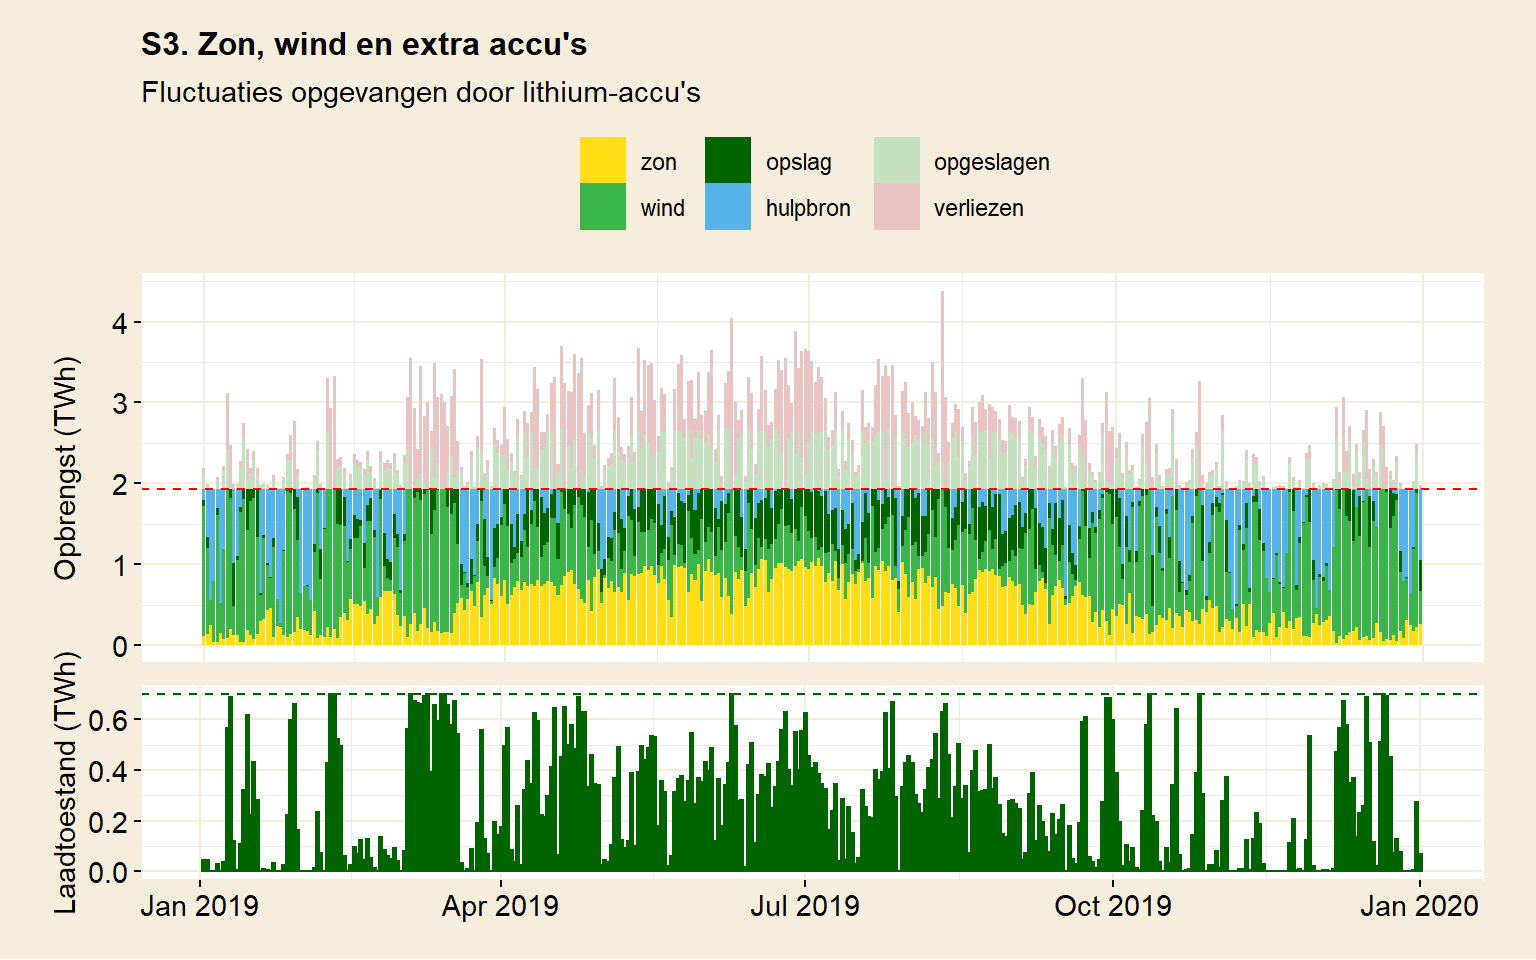
\includegraphics{06-Simulaties_files/figure-latex/unnamed-chunk-5-1} 

}

\end{figure}

De simulatie (figuur S3) laat zien in welke mate deze buffercapaciteit in staat is de fluctuaties van zon en wind op te vangen. Het blijkt dat de capaciteit aan lithium-accu's ter grootte van het gehele wagenpark van Nederland onvoldoende is. De figuur toont dat de accu vaak leeg of bijna leeg is. Te zien is aan de blauwe gebieden in het jaarverloop dat er frequent nog gebruik wordt gemaakt van een hulpbron om de tekorten aan te vullen. In totaal dekt de accu nu 15\% van de energielevering en de hulpbron 18\% (zie tabel 5.2). Het maximale laadvermogen in dit scenario, 156 \emph{G}W, blijft ruim binnen de marges van de accu's (0,7 \emph{T}W). Laden is dus niet het probleem, maar capaciteit wel.

Werd in scenario 1 (tabel 5.1) nog 33\% van de energiedoor de hulpbron geleverd, nu (in scenario 3) is dat dus gereduceerd tot 18\% . Het tekort halveert dus kennelijk door gebruik te maken van de autoaccu's. Zou het dan zo zijn dat het tekort verdwijnt als deze accucapaciteit twee keer zo groot zou zijn? In scenario S4 is de capaciteit van het wagenpark verdubbeld. Dat vermindert het tekort (en dus het bijdraaien) van 18\% van het jaarlijks verbruik tot 15\%. De situatie verandert er niet wezenlijk door.

Een andere optie is misschien de verdubbeling van de capaciteit van zon en wind in de mix. Om dit te bereiken moet Nederland fictief helemaal worden volgezet met windmolens en zonnecellen bezetten ruim 7\% van Nederland. Dat helpt, zoals te zien is in tabel 5.2, scenario 5. Het tekort wordt nu teruggebracht tot 5\%. Nog steeds blijft een hulpbron noodzakelijk.

Alles bij elkaar leidt het gebruik van een ge-elektrificeerd wagenpark volgens het model niet tot een oplossing. De insteek bij de inrichting van het model was optimistisch. Het gebruik van infrastructuur zit al tegen de marges aan, of zelfs daar overheen. Het zal in werkelijkheid lastig worden om accucapaciteit op deze schaal te realiseren, gezien de hoeveelheid lithium die daarvoor nodig is. Ook het gebruikte landoppervlak zal een stevig debat vergen. Desondanks wordt het doel niet gehaald.

\begin{table}

\caption{\label{tab:unnamed-chunk-6}Zon, wind en lithiumaccu's}
\centering
\fontsize{9}{11}\selectfont
\begin{tabular}[t]{>{}l|>{\raggedleft\arraybackslash}p{2.5cm}>{\raggedleft\arraybackslash}p{2.5cm}>{\raggedleft\arraybackslash}p{2.5cm}}
\toprule
\em{\textbf{\em{}}} & \em{\textbf{S3. zon wind en elektrisch wagenpark}} & \em{\textbf{S4. zon wind en 2x wagenpark}} & \em{\textbf{S5. 2x zon en wind, wagenpark}}\\
\addlinespace[0.3em]
\multicolumn{4}{l}{\textbf{Verbruik}}\\
\em{\hspace{1em}Jaarverbruik} & 706 TWh & 706 TWh & 706 TWh\\
\em{\hspace{1em}Aan waterstof} & 0 \% & 0 \% & 0 \%\\
\em{\hspace{1em}Aan elektriciteit} & 100 \% & 100 \% & 100 \%\\
\addlinespace[0.3em]
\multicolumn{4}{l}{\textbf{Ruimtegebruik}}\\
\em{\hspace{1em}Oppervlakte zon} & 4 \% NL & 4 \% NL & 7 \% NL\\
\em{\hspace{1em}Oppervlakte wind} & 51 \% NL & 51 \% NL & 103 \% NL\\
\addlinespace[0.3em]
\multicolumn{4}{l}{\textbf{Capaciteit}}\\
\em{\hspace{1em}Zon} & 50 \% & 50 \% & 100 \%\\
\em{\hspace{1em}Wind} & 50 \% & 50 \% & 100 \%\\
\em{\hspace{1em}Hulpbron} & 100 \% & 100 \% & 100 \%\\
\em{\hspace{1em}Opslag} & 0.7 TWh & 1.4 TWh & 0.7 TWh\\
\addlinespace[0.3em]
\multicolumn{4}{l}{\textbf{Levering}}\\
\em{\hspace{1em}Zon} & 27 \% & 27 \% & 30 \%\\
\em{\hspace{1em}Wind} & 40 \% & 40 \% & 51 \%\\
\em{\hspace{1em}Hulpbron} & 18 \% & 15 \% & 4.6 \%\\
\em{\hspace{1em}Opslag} & 15 \% & 18 \% & 15 \%\\
\addlinespace[0.3em]
\multicolumn{4}{l}{\textbf{Verliezen}}\\
\em{\hspace{1em}Onbenut zon \& wind} & 12 \% & 8 \% & 99 \%\\
\em{\hspace{1em}Omzettingsverliezen} & 6 \% & 7 \% & 6 \%\\
\bottomrule
\multicolumn{4}{l}{\rule{0pt}{1em}Voor een toelichting op de tabel, zie einde van dit hoofdstuk.}\\
\end{tabular}
\end{table}

\newpage

\hypertarget{hoe-effectief-is-windenergie-op-land}{%
\subsection{Hoe effectief is windenergie op land?}\label{hoe-effectief-is-windenergie-op-land}}

Windenergie heeft een relatief lage energiedichtheid. Om de energie te produceren die in 2019 verbruikt werd, zou Nederland volgens het model meer dan volgezet moeten worden met windmolens (Tabel 5.3, S6). Het ruimtegebruik van windmolens is dus aanzienlijk. Nederland is een klein land en het gebruikt veel energie. De fluctuaties worden voor nu buiten beschouwing gelaten.

Met `Nederland' wordt hier het landoppervlak van Nederland bedoeld, inclusief Waddenzee, de Zeeuwse stromen, IJsselmeer en Markermeer (figuur 2.3). Er is in Nederland weinig ongebruikte grond te vinden. Daar staat tegenover dat na de plaatsing van windmolens de ruimte nog gebruikt kan worden voor andere doeleinden. Dat is een voordeel dat zonnepanelen niet hebben. Het is wel zo dat iedere windmolen bereikbaar moet zijn voor onderhoud. Er moet een weg naartoe liggen. In de simulatie staan de windmolens 875 meter uit elkaar. Dat betekent dus dat in de gebruikte ruimte er om de 875 meter een weg zal moeten worden aangelegd.

Het CBS houdt ons \href{https://opendata.cbs.nl/statline/?dl=FB31\#/CBS/nl/dataset/70262ned/table}{ruimtegebruik} bij. In 2015 was dat: Agrarisch terrein (54\%), Bos en open natuurlijk terrein (12\%), Buitenwater en Binnenwater (19\%), Bebouwd terrein (9\%), Verkeersterrein (3\%), Recreatieterrein (3\%) en Semi-bebouwd terrein (1\%).

\begin{figure}
\centering
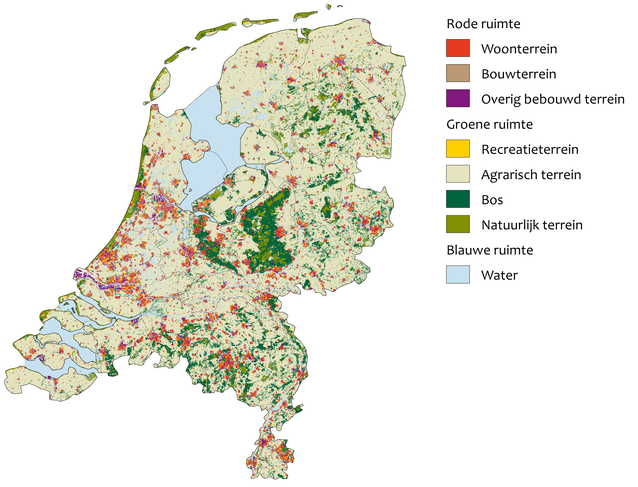
\includegraphics{bodemkaartNL.png}
\caption{Figuur 5.3. Bodemgebruikskaart voor Nederland (2015). Bron: CBS/Kadaster, \href{https://www.clo.nl/indicatoren/nl0061-bodemgebruikskaart-voor-nederland}{Compendium voor de Leefomgeving}}
\end{figure}

De vraag is waar windmolens geplaatst kunnen worden zonder dat de huidige functies van de gebruikte ruimte in het geding komen. Plaatsing in bos en natuurgebieden zullen velen misschien niet ideaal vinden. De Oosterschelde en de Waddenzee vallen beiden onder natuurgebied. Dat geldt niet voor het IJsselmeer en het Markermeer, maar die beslaan samen slechts 4,4\% van Nederland. Wellicht is landbouwgebied een optie, dat beslaat 54\% van Nederland. Hoe dan ook, een dergelijk ruimtegebruik zal offers vragen.

De afweging die gemaakt zou moeten worden, is of de lage opbrengst van windenergie de offers ook waard is. Een betekenisvolle bijdrage van windenergie heeft als consequentie dat er in een groot gedeelte van Nederland windmolens komen te staan. Zelfs als onderdeel van de energiemix, bijvoorbeeld als de andere helft van de energievraag door zon of kernenergie geleverd zou worden, blijft de helft van Nederland nodig. Om dit in perspectief te brengen: de provincie Noord-Holland beslaat ongeveer 10\% van Nederland. Het model gaat uit van molens die 875 meter uit elkaar staan en 200 meter hoog zijn. In vijf provincies zou er dus om de 875 meter een molen worden geplaatst. Dat is hoe er ook tegen aan wordt gekeken veel ruimte. Dit ruimtegebruik is eigenlijk alleen verder te beperken door het energieverbruik te verminderen.

Hoe zit het met windenergie op zee? Het model kan dat niet precies berekenen omdat de fijnmazige gegevens daarvoor ontbreken. Er kan wel gerekend worden op de achterkant van de envelop, als wordt aangenomen dat de \emph{variatie} in wind op zee gelijk is aan die op land. Onder die aanname is te verwachten dat de opbrengst op zee het dubbele is van die op land (zie hoofdstuk wind). Dat zou betekenen dat windenergie op zee de helft van het oppervlakte gebruikt. Het Nederlandse gedeelte van het \href{https://nl.wikipedia.org/wiki/Nederlandse_Exclusieve_Economische_Zone}{continentaal plat} is iets groter dan Nederland zelf (135\%). Volgens \href{https://nl.wikipedia.org/wiki/Windturbines_in_Nederland}{wikipedia} is 40\% daarvan te gebruiken voor windmolens. Als de windmolens uit scenario 6 van land naar zee worden verplaatst, dan zouden deze zo'n 40\% van het plat bezetten. Ongeveer gelijk dus aan de daar beschikbare ruimte.

Dat doet realiseren dat de grenzen voor windcapaciteit in Nederland aardig snel bereikt worden, als dat in prespectief wordt gebracht met de hoeveelheid energie die Nederland gebruikt. Het betekent ook dat de ruimte voor overcapaciteit beperkt is, zelfs als men daarvoor zou uitwijken naar zee. Dat verhoudt zich minder gunstig met scenario's waarbij overcapaciteit in windenergie vereist wordt.

Zou zonne-energie gezien dit alles dan niet een veel efficiëntere keuze zijn? Uit het model blijkt dat 7\% van NL nodig zou zijn om het jaarverbruik met zonnecellen op te wekken (Tabel 3, S7). Zonne-energie brengt per vierkante kilometer 14 keer meer op. Kunnen we windenergie maar beter laten varen en in plaats daarvan vol inzetten op zonne-energie? Dat is een goede vraag, waar apart op wordt ingegaan.

\begin{table}

\caption{\label{tab:unnamed-chunk-7}}
\centering
\fontsize{9}{11}\selectfont
\begin{tabular}[t]{>{}l|>{\raggedleft\arraybackslash}p{2.5cm}>{\raggedleft\arraybackslash}p{2.5cm}}
\toprule
\em{\textbf{\em{}}} & \em{\textbf{S6. Alleen windenergie}} & \em{\textbf{S7. Alleen zonne-energie}}\\
\addlinespace[0.3em]
\multicolumn{3}{l}{\textbf{Verbruik}}\\
\em{\hspace{1em}Jaarverbruik} & 706 TWh & 706 TWh\\
\em{\hspace{1em}Aan waterstof} & 0 \% & 0 \%\\
\em{\hspace{1em}Aan elektriciteit} & 100 \% & 100 \%\\
\addlinespace[0.3em]
\multicolumn{3}{l}{\textbf{Ruimtegebruik}}\\
\em{\hspace{1em}Oppervlakte zon} & 0 \% NL & 7 \% NL\\
\em{\hspace{1em}Oppervlakte wind} & 103 \% NL & 0 \% NL\\
\addlinespace[0.3em]
\multicolumn{3}{l}{\textbf{Capaciteit}}\\
\em{\hspace{1em}Zon} & 0 \% & 100 \%\\
\em{\hspace{1em}Wind} & 100 \% & 0 \%\\
\em{\hspace{1em}Hulpbron} & 100 \% & 100 \%\\
\em{\hspace{1em}Opslag} & 0 TWh & 0 TWh\\
\addlinespace[0.3em]
\multicolumn{3}{l}{\textbf{Levering}}\\
\em{\hspace{1em}Zon} & 0 \% & 38 \%\\
\em{\hspace{1em}Wind} & 61 \% & 0 \%\\
\em{\hspace{1em}Hulpbron} & 39.4 \% & 62.1 \%\\
\em{\hspace{1em}Opslag} & 0 \% & 0 \%\\
\addlinespace[0.3em]
\multicolumn{3}{l}{\textbf{Verliezen}}\\
\em{\hspace{1em}Onbenut zon \& wind} & 39 \% & 62 \%\\
\em{\hspace{1em}Omzettingsverliezen} & 0 \% & 0 \%\\
\bottomrule
\multicolumn{3}{l}{\rule{0pt}{1em}Voor een toelichting op de tabel, zie einde van dit hoofdstuk.}\\
\end{tabular}
\end{table}

\newpage

\hypertarget{schone-energie-zonder-kernenergie-kan-dat}{%
\subsection{Schone energie zonder kernenergie: kan dat?}\label{schone-energie-zonder-kernenergie-kan-dat}}

Kernenergie kan worden ingezet om de opbrengstfluctuaties van zon en wind op te vangen. Kernenergie is eigenlijk het enige alternatief om continu energie te kunnen produceren, zonder dat daarbij CO\textsubscript{2} wordt uitgestoten. Als kernenergie niet wordt ingezet, dan moeten de fluctuaties in de energievoorziening op een andere manier worden opgevangen. Energieopslag is dan de enig resterende oplossing.

Eerder werd gezien dat opslag in accu's en spaarbekkens serieuze limitaties hebben. Grondstoffen vormen een beperkende factor in het gebruik van accu's. Voor spaarbekkens geldt dat de geografische situatie in Nederland (en eigenlijk ook in Europa) zich daar niet goed voor leent (zie hoofdstuk opslag).

Opslag van energie in waterstof heeft wat dat betreft betere kaarten. Er kunnen grotere hoeveelheden energie mee worden opgeslagen. De uitdaging wordt dus om een energiemix samen te stellen gebaseerd op zon, wind en waterstofopslag, die geen gebruik meer maakt van een hulpbron. Dat zou uit het oogpunt van infrastructuur goed nieuws zijn, want het scheelt de plaatsing van hulpcentrales.

In deze simulatie wordt er van uitgegaan dat de maatschappij voor 25\% draait op waterstof, en voor 75\% op elektriciteit. In de energietransitie zullen niet alle processen ge-elektrificeerd kunnen worden, dus enig verbruik in waterstof is realistisch. De verhouding is vrij willekeurig gekozen, met een voorkeur voor elektriciteit. Een ge-elektrificeerd proces is vaak efficiënter dan een waterstofgebaseerd proces.

Begin met min of meer het 'standaard'scenario: een gelijke hoeveelheid wind en zon, zodanig dat ons gemiddelde energieverbruik wordt gedekt. Het resultaat is te zien in figuur S8. Direct is duidelijk dat in deze eerste simulatie de opzet nog niet slaagt (tabel 5.4). De hulpbron moet worden aangesproken om tekorten aan te vullen.

\begin{figure}

{\centering 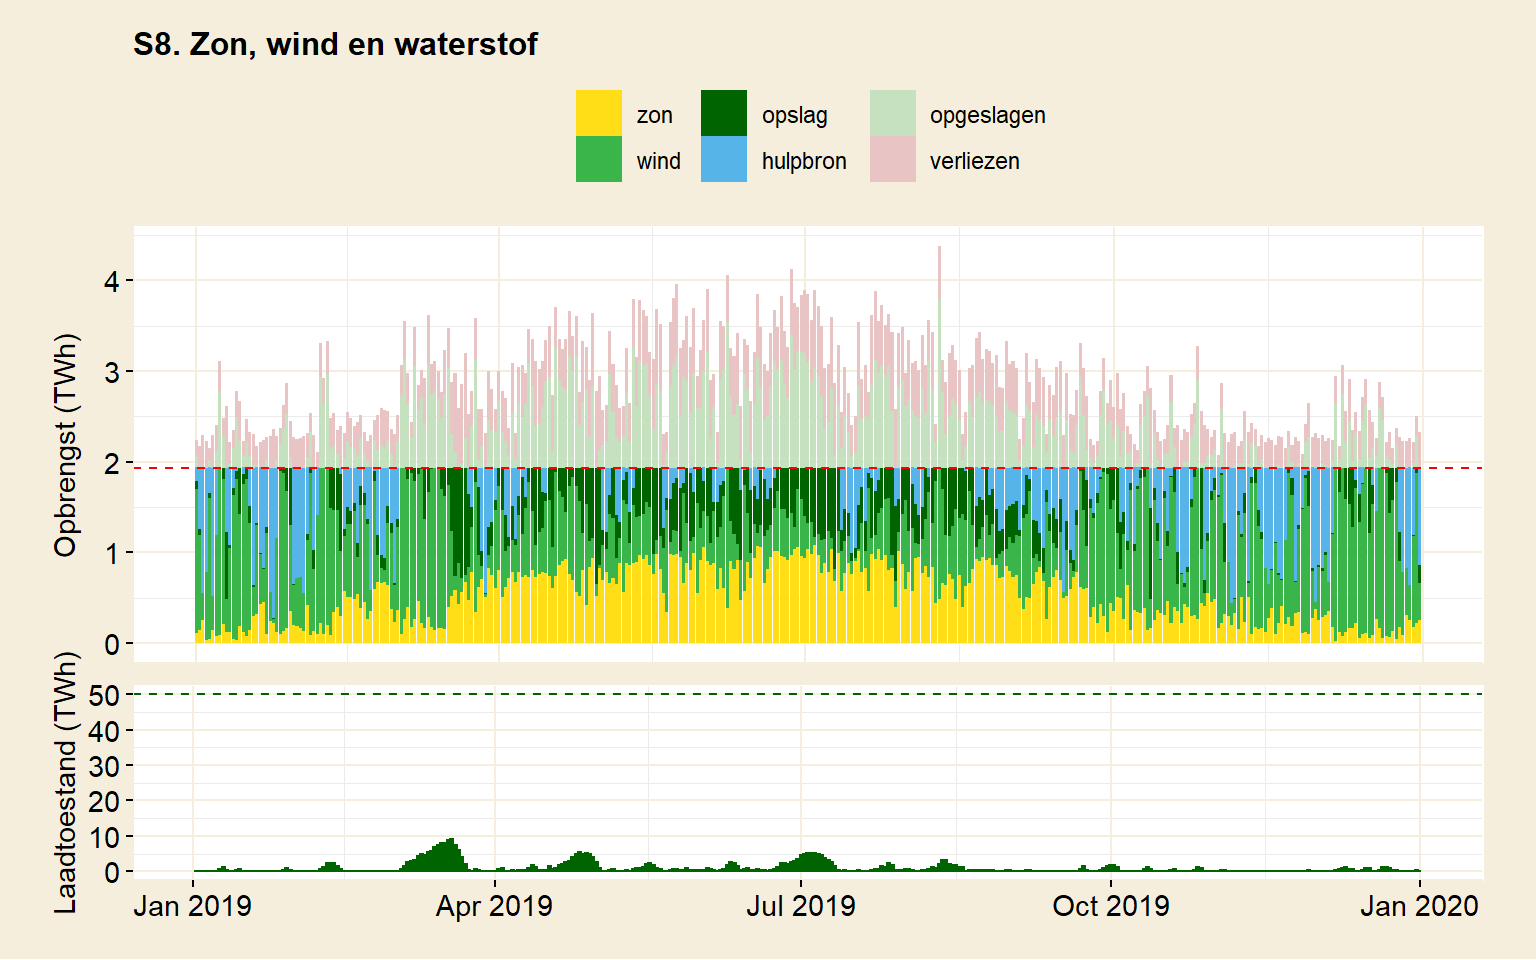
\includegraphics{06-Simulaties_files/figure-latex/unnamed-chunk-8-1} 

}

\end{figure}

De opslag die hier wordt gesimuleerd is 50 TWh groot. Dat is een krappe maand aan energieverbruik, best veel dus. De opslag raakt echter niet vol.~Hoe komt dat? Er gaat wat energie verloren aan de productie van waterstof. Datzelfde geldt voor het leveren van elektriciteit uit de opslag. Beide hebben te maken met efficiëntieverlies van omzettingen en die zijn niet te vermijden. Daarnaast blijkt dat alle overschot van energie uit wind en zon wordt benut (tabel 5.4, S8, \emph{onbenut}). Dat moet dan betekenen dat er niet voldoende capaciteit is om de opslag te vullen.

De voor de hand liggende stap is om de energieproductie te vergroten. In scenario S9 wordt de hoeveelheid zonnecellen verdubbeld. Het aantal windmolens blijft hetzelfde. De opslag wordt uitgebreid tot 150 TWh.

\begin{figure}

{\centering 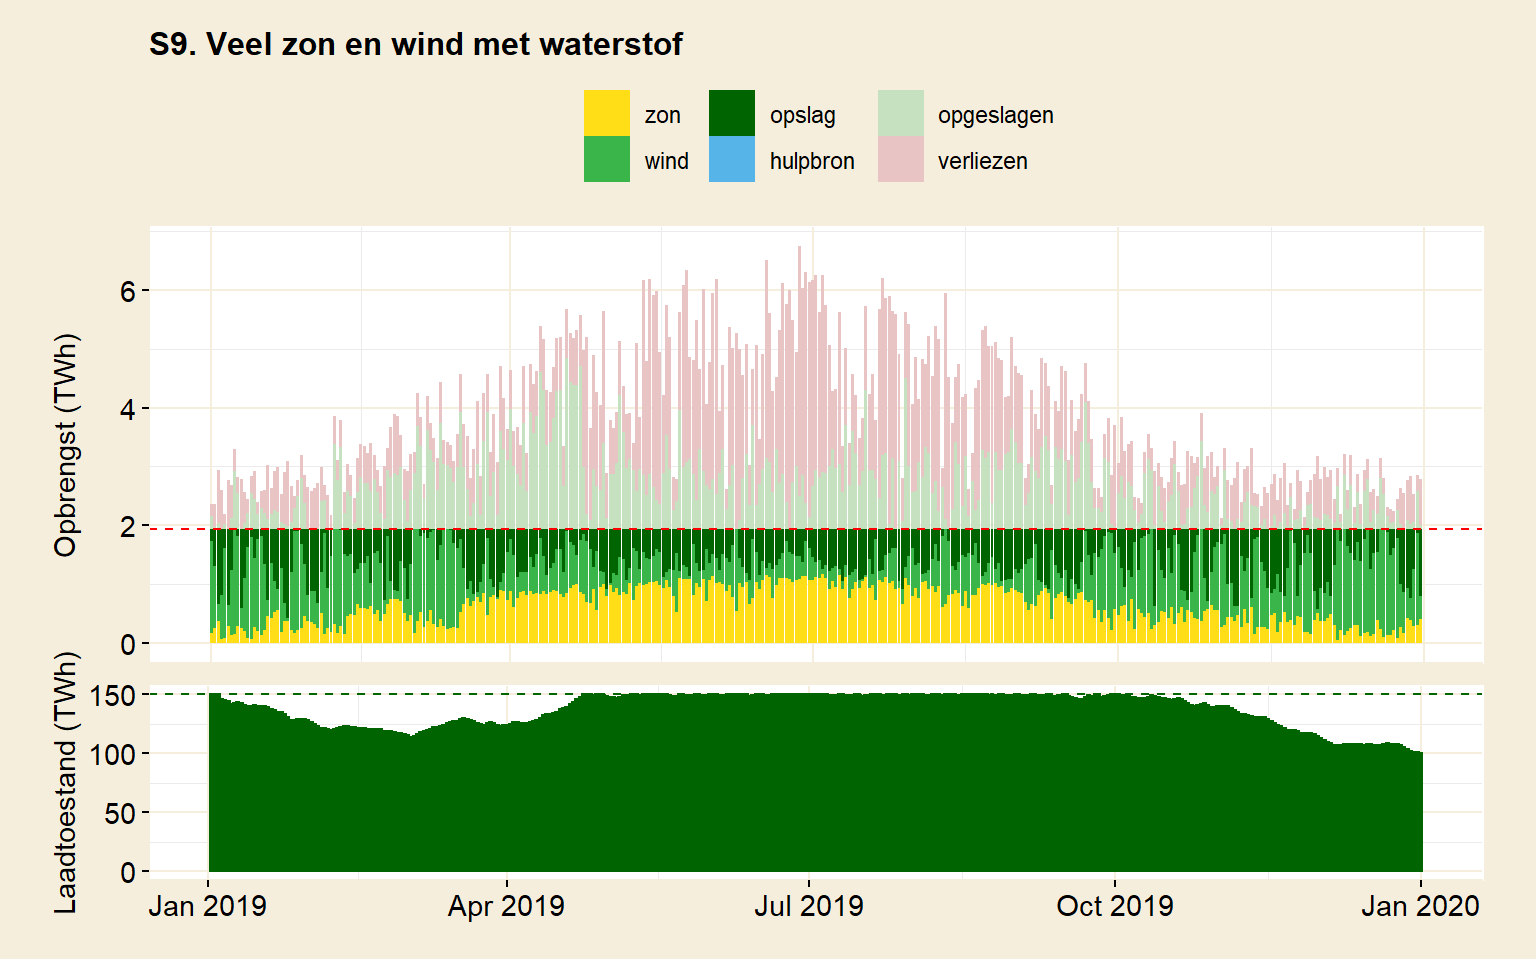
\includegraphics{06-Simulaties_files/figure-latex/unnamed-chunk-9-1} 

}

\end{figure}

Nu kan de simulatie het wèl zonder hulpbron doen (figuur S9). Om te zien of dit ook voor een langere periode geldt, word de simulatie herhaald met dezelfde configuratie. Figuur S10 toont het verloop tussen begin 2001 en eind 2019. Ook over deze langere periode hoeft de hulpbron niet bij te draaien. Te zien is aan de minima van de laadtoestand in figuur S10 dat de opslag niet veel kleiner dan 150 TWh kan zijn. Meer reserve aanhouden zou op zich dus geen slecht idee zijn. In 2017 komt de bodem in zicht, een slechter jaar kan deze opslag niet meer aan.

Goed, wat staat er nu uiteindelijk aan infrastructuur om dit resultaat te bereiken? Windmolens staan op grofweg de helft van het landoppervlak (of 20\% van het continentaal plat). Het model rekent voor het oppervlaktegebruik van zonnecellen 8\% van Nederland (zonder tussenruimte). Dat is een oppervlak ter grootte van de provincie Zuid-Holland. Zonnecellen zijn lastig te combineren met ander grondgebruik. Misschien dat daar landbouwgrond voor moet worden opgeofferd?

De noodzakelijke hoeveelheid opslag is alleen te realiseren door gebruik te maken van waterstof. De gebruikte 150 TWh is vergelijkbaar met tweeëneenhalve maand aan nationaal energieverbruik. De benodigde opslagcapaciteit is enorm. Een dergelijke capaciteit is met accu's onmogelijk te realiseren.

Maar ook de realisatie via waterstof kent zijn uitdagingen. Er is uitgebreide en diverse infrastructuur nodig om dat voor elkaar te krijgen. Hieronder wordt daar een schatting van gemaakt.

Begin met de waterstofproductie, die gebeurt met behulp van electrolysers. Neem aan dat een waterstoffabriek een vermogen van 100 MW heeft (`s werelds grootste heeft een vermogen 20 MW. In Nederland leeft de \href{https://www.technischweekblad.nl/nieuws/uniper-en-haven-overwegen-waterstoffabriek-van-100-mw}{ambitie} om in 2025 naar 100 MW te schalen). Hoeveel zijn er daar van nodig? Om dat te schatten kan er worden gekeken naar het piekvermogen waarmee de waterstofopslag werd geladen. Dat piekvermogen moet door de waterstoffabrieken kunnen worden verwerkt, wil er geen energie verloren gaan. Een conservatieve schatting geeft als piekvermogen 330 GW aan, wat neerkomt op 3300 waterstoffabrieken (330 / 0,1). (Het piekvermogen werd geschat door het gemiddelde te nemen van de grootste 20\% aan tienminuutsopbrengsten. In de tabel wordt dat aangegeven met 'gemiddeld maximum laadvermogen'. Het absolute maximum wordt ook genoemd, als `maximum laadvermogen'.)

\begin{figure}

{\centering 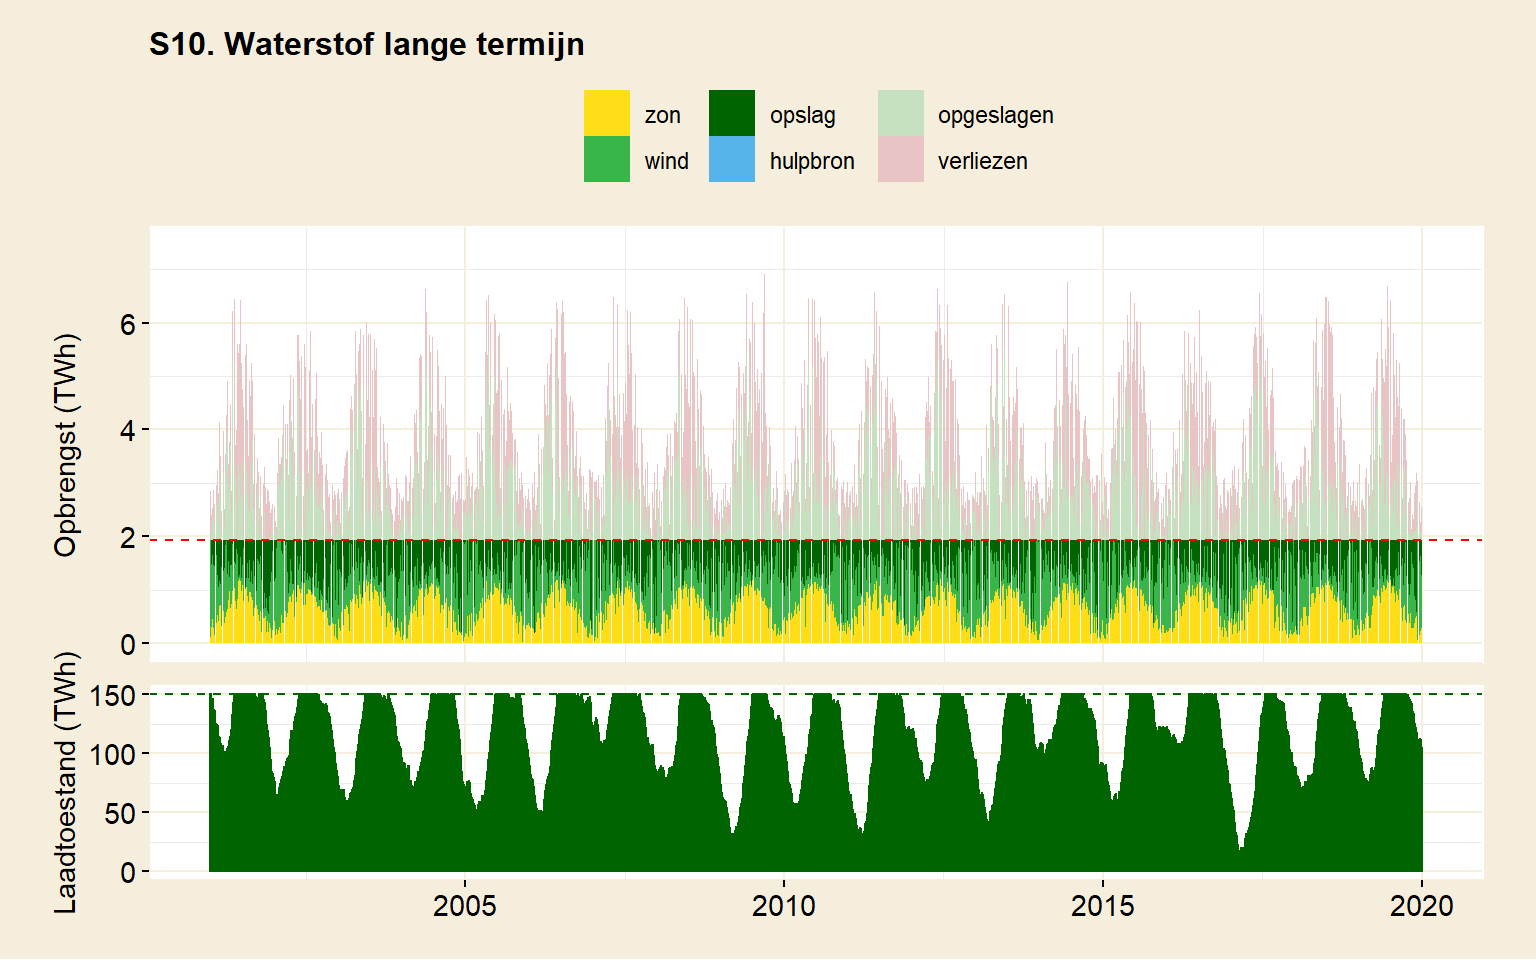
\includegraphics{06-Simulaties_files/figure-latex/unnamed-chunk-10-1} 

}

\end{figure}

Waterstof moet ook weer kunnen worden omgezet in elektriciteit. Als er een elektriciteitstekort onstaat, wordt de opslag aangesproken. Voor productie van elektriciteit moet waterstof worden verbrand (een waterstofcentrale kan vergeleken worden met een gascentrale). Het piekvermogen van de elektricteitsvraag bedroeg 60 GW, goed voor 20 waterstofenergiecentrales van 3 GW (60 / 3).

Compressie en opslag van waterstof vallen buiten de berekeningen van het model. Het piekvermogen dat verwerkt moet worden (330 GW) is 4 keer meer (330 GW / 81 GW)dan Nederland continu verbruikt. De waterstof die op deze momenten geproduceerd wordt moet onder de grond worden gepompt. Vergelijk het met spaarbekkens die voldoende pompen en pijpwerk moeten hebben om genoeg water naar boven te kunnen pompen. Is het haalbaar zo'n groot vermogen op tijd te comprimeren en onder de grond te krijgen?

\bigskip\noindent
Het blijkt dat er voor energieopslag in waterstof veel additionele infrastructuur nodig is. Er zijn fabrieken nodig voor de productie van waterstof en verbrandingscentrales om elektriciteit te kunnen maken. Omdat de gevraagde vermogens hoog zijn, is deze infrastructuur omvangrijk. Dat is vooral het geval bij de productie van waterstof, waar de fabrieken een vermogen aan moeten kunnen dat vier keer groter is dan het nationaal verbruik.

Maar ook de behoefte aan verbrandingscentrales is aanzienlijk. Het model ging er van uit dat de elektriciteitsvraag 75\% van de energiebehoefte betrof (60 GW). Dat vermogen werd in de simulatie ook daadwerkelijk verlangd voor elektriciteitsproductie. Het vermogen van bestaande energiecentrales, even er vanuit gaand dat deze makkelijk voor waterstofverbranding zijn aan te passen, is goed voor 25\% van ons verbruik (zie hoofdstuk verbruik). Dat zou betekenen dat er in dit scenario dus voor 50\% aan ons verbruik moet worden bijgebouwd. Dat is een verdriedubbeling van het aantal bestaande centrales. Ook dat zal een substantiële investering zijn.

Dat telt allemaal op. Een mix zonder kernenergie betaalt in deze simulatie niet alleen voor 150\% aan vermogen in wind- en zonne-energie, maar ook voor 409\% aan vermogen in waterstoffabrieken en vervolgens nog 75\% aan vermogen in verbrandingscentrales. Dat er aan deze stapeling van infrastructuur een prijskaartje hangt, is niet onaannemelijk. De huidige situatie op basis van fossiele brandstoffen vergt een investering in infrastructuur die proportioneel is met 100\% van ons vermogen. Bij gelijke kosten voor infrastructuur zou de energievoorziening dus meer dan zes keer duurder worden dan nu het geval is. (De kosten voor de verschillende vormen van infrastructuur zijn natuurlijk niet hetzelfde. Het bepalen van de exacte kosten voor infrastructuur is echter lastig. De benadering hier gaat uit van kosten voor \emph{vermogen} in plaats van het noemen van een bedrag. De relatie zal niet één op één zijn, maar het is aannemelijk dat als er betaald moet worden voor diverse infrastructuur die 6x het verbruik van Nederland moet dekken, dat aanzienlijk meer gaat kosten dan een situtatie waar infrastructuur nodig is die ons verbruik 1x dekt.)

\bigskip\noindent
Tot slot dan: kan duurzame energie inderdaad zonder kernenergie? Dat hangt af van het vertrouwen dat men heeft in toekomstige technische ontwikkelingen. De techniek staat op veel vlakken nog in de kinderschoenen. Het verkrijgen van een inschatting of grote hoeveelheden waterstof voldoende snel zijn op te slaan in de praktijk is daarbij cruciaal. Als dat niet lukt, dan is deze opslagmethode geen oplossing voor het probleem. Ook het tijdspad tot een goede oplossing is onduidelijk. Een tweede punt is dat men bereid zal moeten zijn te betalen voor extra de infrastructuur die deze oplossing met zich meebrengt.

\begin{table}

\caption{\label{tab:unnamed-chunk-11}Zon, wind en waterstofopslag}
\centering
\fontsize{9}{11}\selectfont
\begin{tabular}[t]{>{}l|>{\raggedleft\arraybackslash}p{2.5cm}>{\raggedleft\arraybackslash}p{2.5cm}>{\raggedleft\arraybackslash}p{2.5cm}}
\toprule
\em{\textbf{\em{}}} & \em{\textbf{S8. Zon, wind en waterstof}} & \em{\textbf{S9. Veel zon en wind met waterstof}} & \em{\textbf{S10. Waterstof lange termijn}}\\
\addlinespace[0.3em]
\multicolumn{4}{l}{\textbf{Verbruik}}\\
\em{\hspace{1em}Jaarverbruik} & 706 TWh & 706 TWh & 706 TWh\\
\em{\hspace{1em}Aan waterstof} & 25 \% & 25 \% & 25 \%\\
\em{\hspace{1em}Aan elektriciteit} & 75 \% & 75 \% & 75 \%\\
\addlinespace[0.3em]
\multicolumn{4}{l}{\textbf{Ruimtegebruik}}\\
\em{\hspace{1em}Oppervlakte zon} & 4 \% NL & 7 \% NL & 8 \% NL\\
\em{\hspace{1em}Oppervlakte wind} & 51 \% NL & 51 \% NL & 52 \% NL\\
\addlinespace[0.3em]
\multicolumn{4}{l}{\textbf{Capaciteit}}\\
\em{\hspace{1em}Zon} & 50 \% & 100 \% & 100 \%\\
\em{\hspace{1em}Wind} & 50 \% & 50 \% & 50 \%\\
\em{\hspace{1em}Hulpbron} & 100 \% & 0 \% & 0 \%\\
\em{\hspace{1em}Opslag} & 50 TWh & 150 TWh & 150 TWh\\
\addlinespace[0.3em]
\multicolumn{4}{l}{\textbf{Levering}}\\
\em{\hspace{1em}Zon} & 27 \% & 33 \% & 33 \%\\
\em{\hspace{1em}Wind} & 40 \% & 37 \% & 37 \%\\
\em{\hspace{1em}Hulpbron} & 17.7 \% & 0 \% & 0 \%\\
\em{\hspace{1em}Opslag} & 15 \% & 30 \% & 30 \%\\
\addlinespace[0.3em]
\multicolumn{4}{l}{\textbf{Verliezen}}\\
\em{\hspace{1em}Onbenut zon \& wind} & 0 \% & 26 \% & 17 \%\\
\em{\hspace{1em}Omzettingsverliezen} & 22 \% & 31 \% & 33 \%\\
\addlinespace[0.3em]
\multicolumn{4}{l}{\textbf{Draaitijd hulpbron}}\\
\em{\hspace{1em}Totale draaitijd} & 29.3 \% & 0 \% & 0 \%\\
\em{\hspace{1em}Draaitijd op > 90\% verm.} & 5.8 \% & 0 \% & 0 \%\\
\addlinespace[0.3em]
\multicolumn{4}{l}{\textbf{Laadvermogen opslag}}\\
\em{\hspace{1em}Maximaal} & 359 GW & 655 GW & 750 GW\\
\em{\hspace{1em}Gemiddelde top 20\%} & 164 GW & 307 GW & 330 GW\\
\em{\hspace{1em}Max. ontladen elektr.} & 45 GW & 45 GW & 45 GW\\
\addlinespace[0.3em]
\multicolumn{4}{l}{\textbf{Inventaris}}\\
\em{\hspace{1em}Hulpcentrales (3 GW)} & 27 & 0 & 0\\
\em{\hspace{1em}Waterstoffabrieken (100 MW)} & 1642 & 3067 & 3298\\
\em{\hspace{1em}Waterstofcentrales (3 GW)} & 20 & 20 & 20\\
\em{Periode} & 2019 & 2019 & 2001 - 2019\\
\bottomrule
\multicolumn{4}{l}{\rule{0pt}{1em}Voor een toelichting op de tabel, zie einde van dit hoofdstuk.}\\
\end{tabular}
\end{table}

\newpage

\hypertarget{hoe-ziet-een-energiemix-met-alleen-kernenergie-er-uit}{%
\subsection{Hoe ziet een energiemix met alleen kernenergie er uit?}\label{hoe-ziet-een-energiemix-met-alleen-kernenergie-er-uit}}

Kernenergie is een continue energiebron. In tegenstelling tot variabele bronnen is het in staat op ieder moment aan onze energiebehoefte te voldoen. Dat geldt ook als de energiebehoefte niet constant zou zijn. De energielevering is daarop aan te passen.

Dat betekent dat de problematiek rondom fluctuaties bij kernenergie niet speelt. Uit het oogpunt van energielevering is een energiemix die enkel bestaat uit kernenergie met afstand de meest eenvoudige. Er is geen extra infrastructuur nodig om de energievoorziening op peil te houden. De investering blijft beperkt tot een 100\% dekkend vermogen aan kerncentrales. Om Nederland van energie te voorzien volstaan 27 kerncentrales van 3 GW (de grootte van de kerncentrale in Doel, net over de Belgische grens). Deze centrales nemen tezamen een ruimte in van 21 km\textsuperscript{2} (berekend aan de hand van de oppervlaktebezetting van de \href{https://nl.wikipedia.org/wiki/Kerncentrale_Doel}{centrale in Doel}).

Kerncentrales produceren elektriciteit. In de energietransitie zullen niet alle processen ge-elektrificeerd kunnen worden. Er blijft een schone brandstof nodig. Dat wordt waarschijnlijk waterstof. Er zal dan infrastructuur nodig zijn voor de productie van waterstof. Het aantal waterstoffabrieken dat nodig is, zal moeten aansluiten op de vraag. In scenario 8 werd er vanuit gegaan dat de maatschappij voor 25\% van haar energiegebruik afhankelijk is van waterstof. Om dat verbruik aan te kunnen zijn 202 waterstoffabrieken à 100 MW nodig.

Omdat kernenergie een continue energiebron is, kan het waterstof geproduceerd worden wanneer het nodig is. Er hoeft dus geen opslagcapaciteit te zijn. Datzelfde geldt voor waterstofenergiecentrales, want er hoeft geen stroom opgewekt te worden uit opslag.

Kernenergie is een schone bron in de zin dat het geen CO\textsubscript{2} uitstoot. Het is onwaarschijnlijk dat er snel een \href{https://www.scientificamerican.com/article/how-long-will-global-uranium-deposits-last/}{tekort aan brandstof} (uranium) zal onstaan. In die zin is kernenergie als duurzaam te beschouwen. Historisch gezien is kernenergie even veilig als wind- en zonne-energie (zie \href{https://ourworldindata.org/safest-sources-of-energy}{Our world in data}). Vanuit een veiligheidsstandpunt redt het zelfs levens als het fossiele energiebronnen vervangt.

\begin{figure}

{\centering 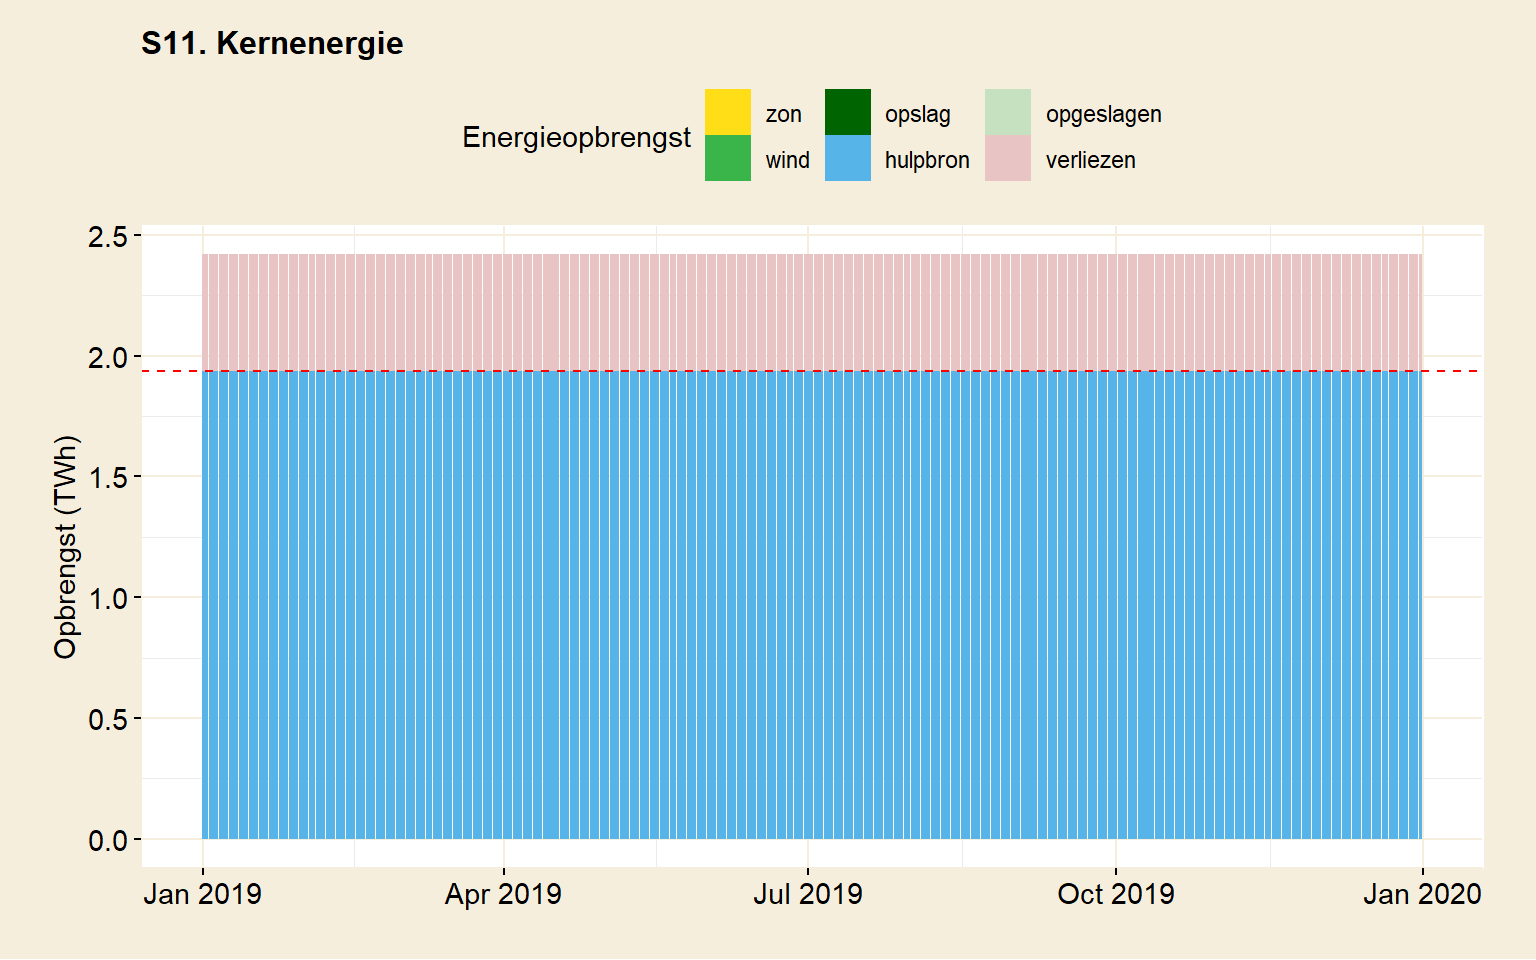
\includegraphics{06-Simulaties_files/figure-latex/unnamed-chunk-12-1} 

}

\end{figure}

\hypertarget{kan-beperkte-inzet-van-kernenergie-de-fluctuaties-van-wind-en-zon-opvangen}{%
\subsection{Kan beperkte inzet van kernenergie de fluctuaties van wind en zon opvangen?}\label{kan-beperkte-inzet-van-kernenergie-de-fluctuaties-van-wind-en-zon-opvangen}}

Zou het mogelijk zijn een beperkt aantal kerncentrales in te zetten als achtervang bij fluctuerende bronnen, zonder daarbij energieopslag te gebruiken? Massa-opslag is complex en op de benodigde schaal bovendien nog onbewezen. Het gebruik van een continue hulpbron is het andere alternatief om de energielevering te kunnen blijven garanderen. Deze energiecentrales zouden op fossiele brandstoffen kunnen draaien, maar het doel van de energietransitie was nu juist om dat te vermijden. De alternatieve hulpbron die dan overblijft is kernenergie.

Een beperkte inzet van kernenergie betekent dat wind en zon qua energieproductie meer op hun schouders moeten nemen. We willen er immers voor zorgen dat er zo min mogelijk kerncentrales staan. Het opvoeren van de capaciteit van wind en zon lijkt een logische manier om het aantal benodigde kerncentrales te doen afnemen.

Maar dat idee blijkt niet helemaal te kloppen. Op een mistige, windloze winterdag zou de opbrengst van zon en wind nihil zijn. De kerncentrales die worden ingezet om het gat te vullen, krijgen de volle last van de vraag op hun schouders. Het is niet zozeer hoe lang de kerncentrales moeten worden ingezet, maar juist hoeveel vermogen er op dat moment wordt gevraagd. Al blijft het tekort bij dit enige, mistige etmaal en staan de kerncentrales de rest van het jaar stil, om het gevraagde vermogen te kunnen leveren zijn toch veel kerncentrales nodig.

In scenario 12 (tabel 5.5) is bekeken hoeveel kerncentrales er nodig zijn onder de aanname dat wind- en zonne-energie de energievraag dekken. Over de gehele periode produceren wind en zon precies genoeg energie om aan de vraag te voldoen. De kerncentrales worden dus alleen gebruikt om de gaten op te vangen.

Scenario 12 laat zien dat er 27 kerncentrales nodig zijn. Dat aantal is voldoende om Nederland van energie te voorzien, zelfs zonder hulp van wind en zon. Het doel van beperkte kernenergie wordt met dit scenario nog niet bereikt. Sterker nog, de inzet van de centrales is maximaal.

De momenten waarop de kerncentrales draaien, en vooral het vermogen waarmee dat gebeurt, moeten dus worden teruggebracht. Hoe vaak zijn de centrales eigenlijk actief? Het model meet de tijd dat een hulpron actief was en op welk vermogen dat gebeurde. Daarvoor werd de periode van 2015 tot en met 2019 doorgerekend. Scenario 12 laat zien dat de kerncentrales 10\% van de tijd meer dan 90\% van het gevraagde vermogen leveren. Zo'n 36 dagen per jaar wordt er dus van alle 27 centrales vol vermogen gevraagd.

De enige optie die openstaat om hier verandering in te brengen, is om de opbrengst uit wind en zon te vergroten. Zoals eerder gezien is het genereren van overcapaciteit niet makkelijk. De vraag is hoe ver men wil gaan.

In scenario 13 wordt gerekend met een extreem scenario waarbij windmolens alle landbouwgrond (de helft van Nederland) en het volledige bruikbare continentale plat beslaan (40\% van het landoppervlak. In de simulatie is dit oppervlak verdubbeld, om de twee keer zo hoge opbrengst op zee te benaderen). Daarnaast wordt een kwart van de landbouwgrond met zonnecellen bedekt. Wind en zon wekken in dit scenario tezamen vijf keer meer energie op dan Nederland in de periode verbruikt.

Toch blijft het om uitval te voorkomen 5\% van de tijd nodig om 27 kerncentrales op vol vermogen te laten draaien. Het aantal benodigde centrales wordt niet minder, alleen het aantal dagen dat ze ingezet moeten worden.
Het idee was om het aantal centrales te beperken. Ook in dit extreme scenario blijkt dat volgens het model niet haalbaar. Het lijkt alles of niets te zijn. Of er staan kerncentrales die de gehele energievraag aankunnen, of de energievoorziening hapert.

Het alternatief van (weinig) kerncentrales werd deels ingegeven om de complexiteit van opslag in waterstof te vermijden. Maar misschien kan beperkt gebruik van opslag in de vorm van (lithium)accu's wel helpen. De capaciteit die daarmee gerealiseerd kan worden haalt het niet bij die van waterstof, maar misschien voorkomt het net die perioden -- bijvoorbeeld 's nachts -- waar kerncentrales op vol vermogen moeten draaien.

Scenario S14 voegt 0,7 TWh aan opslag toe aan de simulatie. Dat is gelijk aan de capaciteit van een volledig ge-elektrificeerd wagenpark, zoals elders ook werd gebruikt. Er kan worden getwijfeld of deze opslag erg realistisch is, maar het kan geen kwaad te kijken of het zou helpen. Welnu, in dit nieuwe scenario draaien de kercentrales 1\% van de tijd op vol vermogen (tabel 5.5, S14).

De uitkomsten van het model leiden tot de conclusie dat \emph{beperkte} inzet van kerncentrales geen oplossing biedt. Zelfs de inzet van accu-opslag brengt daar geen verandering in. Het is een alles-of-niets situatie. Het benodigde aantal kerncentrales is maximaal. De capaciteit ervan kan Nederland geheel van energie voorzien. Dat zou wind- en zonne-energie in feite overbodig maken. Wie niet voor kernenergie (op volle capaciteit) wil kiezen, zit vast aan massaopslag om uitval te voorkomen.

\begin{table}

\caption{\label{tab:unnamed-chunk-13}Beperkt kernenergie}
\centering
\fontsize{9}{11}\selectfont
\begin{tabular}[t]{>{}l|>{\raggedleft\arraybackslash}p{2.5cm}>{\raggedleft\arraybackslash}p{2.5cm}>{\raggedleft\arraybackslash}p{2.5cm}}
\toprule
\em{\textbf{\em{}}} & \em{\textbf{S12. Basisscenario beperkt kernenergie}} & \em{\textbf{S13. Extra wind en zon}} & \em{\textbf{S14. Extra wind, zon en beperkte opslag}}\\
\addlinespace[0.3em]
\multicolumn{4}{l}{\textbf{Verbruik}}\\
\em{\hspace{1em}Jaarverbruik} & 706 TWh & 706 TWh & 706 TWh\\
\em{\hspace{1em}Aan waterstof} & 25 \% & 25 \% & 25 \%\\
\em{\hspace{1em}Aan elektriciteit} & 75 \% & 75 \% & 75 \%\\
\addlinespace[0.3em]
\multicolumn{4}{l}{\textbf{Ruimtegebruik}}\\
\em{\hspace{1em}Oppervlakte zon} & 4 \% NL & 25 \% NL & 25 \% NL\\
\em{\hspace{1em}Oppervlakte wind} & 53 \% NL & 158 \% NL & 158 \% NL\\
\addlinespace[0.3em]
\multicolumn{4}{l}{\textbf{Capaciteit}}\\
\em{\hspace{1em}Zon} & 50 \% & 332 \% & 332 \%\\
\em{\hspace{1em}Wind} & 50 \% & 150 \% & 150 \%\\
\em{\hspace{1em}Hulpbron} & 100 \% & 100 \% & 100 \%\\
\em{\hspace{1em}Opslag} & 0 TWh & 0 TWh & 0.7 TWh\\
\addlinespace[0.3em]
\multicolumn{4}{l}{\textbf{Levering}}\\
\em{\hspace{1em}Zon} & 27 \% & 36 \% & 36 \%\\
\em{\hspace{1em}Wind} & 39 \% & 50 \% & 50 \%\\
\em{\hspace{1em}Hulpbron} & 33.5 \% & 13.5 \% & 1.9 \%\\
\em{\hspace{1em}Opslag} & 0 \% & 0 \% & 12 \%\\
\addlinespace[0.3em]
\multicolumn{4}{l}{\textbf{Verliezen}}\\
\em{\hspace{1em}Onbenut zon \& wind} & 31 \% & 391 \% & 374 \%\\
\em{\hspace{1em}Omzettingsverliezen} & 11 \% & 8 \% & 11 \%\\
\addlinespace[0.3em]
\multicolumn{4}{l}{\textbf{Draaitijd hulpbron}}\\
\em{\hspace{1em}Totale draaitijd} & 60.6 \% & 23.7 \% & 2.7 \%\\
\em{\hspace{1em}Draaitijd op > 90\% verm.} & 10 \% & 5 \% & 1 \%\\
\addlinespace[0.3em]
\multicolumn{4}{l}{\textbf{Laadvermogen opslag}}\\
\em{\hspace{1em}Maximaal} & 0 GW & 0 GW & 1319 GW\\
\em{\hspace{1em}Gemiddelde top 20\%} & 0 GW & 0 GW & 370 GW\\
\em{\hspace{1em}Max. ontladen elektr.} & 0 GW & 0 GW & 45 GW\\
\addlinespace[0.3em]
\multicolumn{4}{l}{\textbf{Inventaris}}\\
\em{\hspace{1em}Hulpcentrales (3 GW)} & 27 & 27 & 27\\
\em{\hspace{1em}Waterstoffabrieken (100 MW)} & 0 & 0 & 3696\\
\em{\hspace{1em}Waterstofcentrales (3 GW)} & 0 & 0 & 20\\
\em{Periode} & 2015 - 2019 & 2015 - 2019 & 2015 - 2019\\
\bottomrule
\multicolumn{4}{l}{\rule{0pt}{1em}Voor een toelichting op de tabel, zie einde van dit hoofdstuk.}\\
\end{tabular}
\end{table}

\newpage

\hypertarget{zonne-energie-is-veel-efficiuxebnter-dan-wind.-kunnen-we-het-niet-redden-met-de-zon-alleen}{%
\subsection{Zonne-energie is veel efficiënter dan wind. Kunnen we het niet redden met de zon alleen?}\label{zonne-energie-is-veel-efficiuxebnter-dan-wind.-kunnen-we-het-niet-redden-met-de-zon-alleen}}

Zonne-energie is volgens de simulaties meer dan tien keer efficiënter dan windenergie op land. Uit een vergelijking van scenario's S6 en S7 (tabel 5.3) bleek dat, per vierkante kilometer, zonne-energie 14 keer meer opbrengt dan windenergie op land. Dat ruimtegebruik is een nadeel van windmolens. Bij plaatsing op zee verbetert dat, maar heeft als nadeel dat het een dure optie is. Waarom dan niet enkel de zon gebruiken als energiebron? Dat zou veel minder ruimte innemen. En een veld met zonnecellen valt in het landschap ook nog eens minder op. Is het daarmee niet een voor de hand liggende keuze?

Een nadeel van zonne-energie is dat, hoewel het minder ruimte inneemt dan windmolens, die ruimte niet meer voor andere doeleinden bruikbaar is. Het plaatsen van zonnecellen in een natuurgebied bijvoorbeeld betekent noodzakelijkerwijs de vernietiging van natuur. Plaatsing op oppervlaktewater voorkomt doordringing van licht, wat een nadelige invloed heeft op het leven in het water. Plaatsing op landbouwgrond heeft tot gevolg dat agrarische productie het veld moet ruimen voor energieproductie. Hoewel zonnecellen dus minder ruimte innemen, is de plaatsing ervan ingrijpender.

Zoals bij meer van dit soort vragen maakt schaal uit. Om hoeveel oppervlak gaat het eigenlijk? In scenario 15 wordt een `basisscenario' geschetst waarbij de zon precies genoeg energie produceert om aan de vraag te voldoen. Er wordt geen opslag gebruikt. Acht procent van Nederland wordt gebruikt voor zonnecellen.

\begin{figure}

{\centering 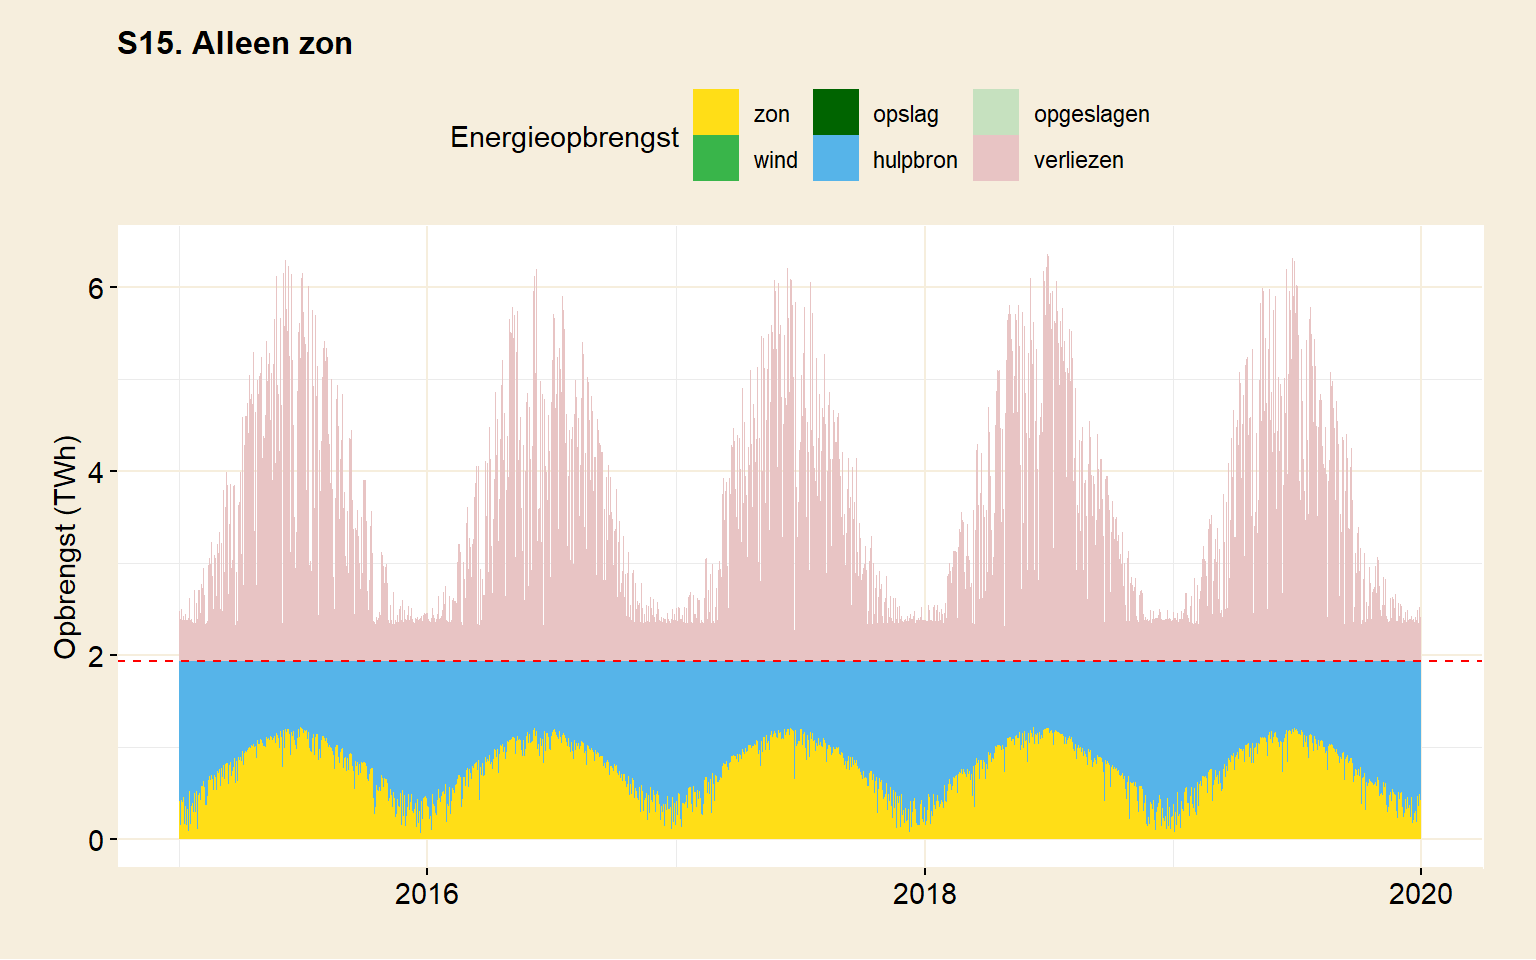
\includegraphics{06-Simulaties_files/figure-latex/unnamed-chunk-14-1} 

}

\end{figure}

Door de breedtegraad waar Nederland op ligt, vindt de energieproductie voornamelijk in de zomer plaats. De winterperiode kenmerkt zich juist door een groot tekort aan energie. De golfbeweging is goed te zien in figuur S15. Om in de winter niet zonder energie te zitten, is er voor die periode een alternatief nodig. Hier wordt dat opgevangen door een hulpbron. Het effect van gebruik van een hulpbron werd elders ook al geconstateerd. Het opgestelde vermogen van de hulpbron moet typisch voldoende zijn om de totale energievraag over te kunnen nemen. Daarnaast moet deze ook nog eens continu beschikbaar zijn. Een schone hulpbron, zoals kernenergie, maakt energieopwekking door een variabele bron overbodig. (Het gebruik van een hulpbron die \emph{niet} schoon is, wordt elders bekeken.)

De andere optie is om opslagcapaciteit te realiseren om de winterperiode door te komen. Het blauw in de figuur geeft de uitdaging mooi aan. De hulpbron is verantwoordelijk voor tweederde van de energieproductie (tabel 5.6) en dat tekort moet opgevangen gaan worden door energieopslag.

Er zijn twee knoppen om aan te draaien: de hoeveelheid zonnecellen en de hoeveelheid opslag. De hulpbron wordt daarbij op nul gehouden. Een grotere opslag betekent dat er minder zonnecellen nodig zijn. Omgekeerd geldt hetzelfde.

Laten we eerst proberen een schatting te maken voor een scenario waarbij het aantal zonnecellen zo klein mogelijk wordt gehouden. Daar kan het model voor worden gebruikt. De capaciteit van de opslag moet dan zo groot mogelijk zijn. Een inschatting van de maximaal haalbare grootte is lastig, omdat waterstofopslag op deze schaal nog niet eerder werd gerealiseerd. In scenario S16 wordt uitgegaan van 350 TWh. Dat is vergelijkbaar met een half jaar nationaal energieverbruik. (Het is moeilijk zo'n hoeveelheid energie te onderschatten. Dat staat gelijk aan 219 keer de \emph{mondiale} opslagcapaciteit in spaarbekkens, die 95\% van de mondiale opslag uitmaken.) Met de eis dat de bijdrage van de hulpbron verwaarloosbaar moet blijven, wordt de minimale hoeveelheid zonnecellen bepaald die de energiehuishouding in balans houdt.

\begin{figure}

{\centering 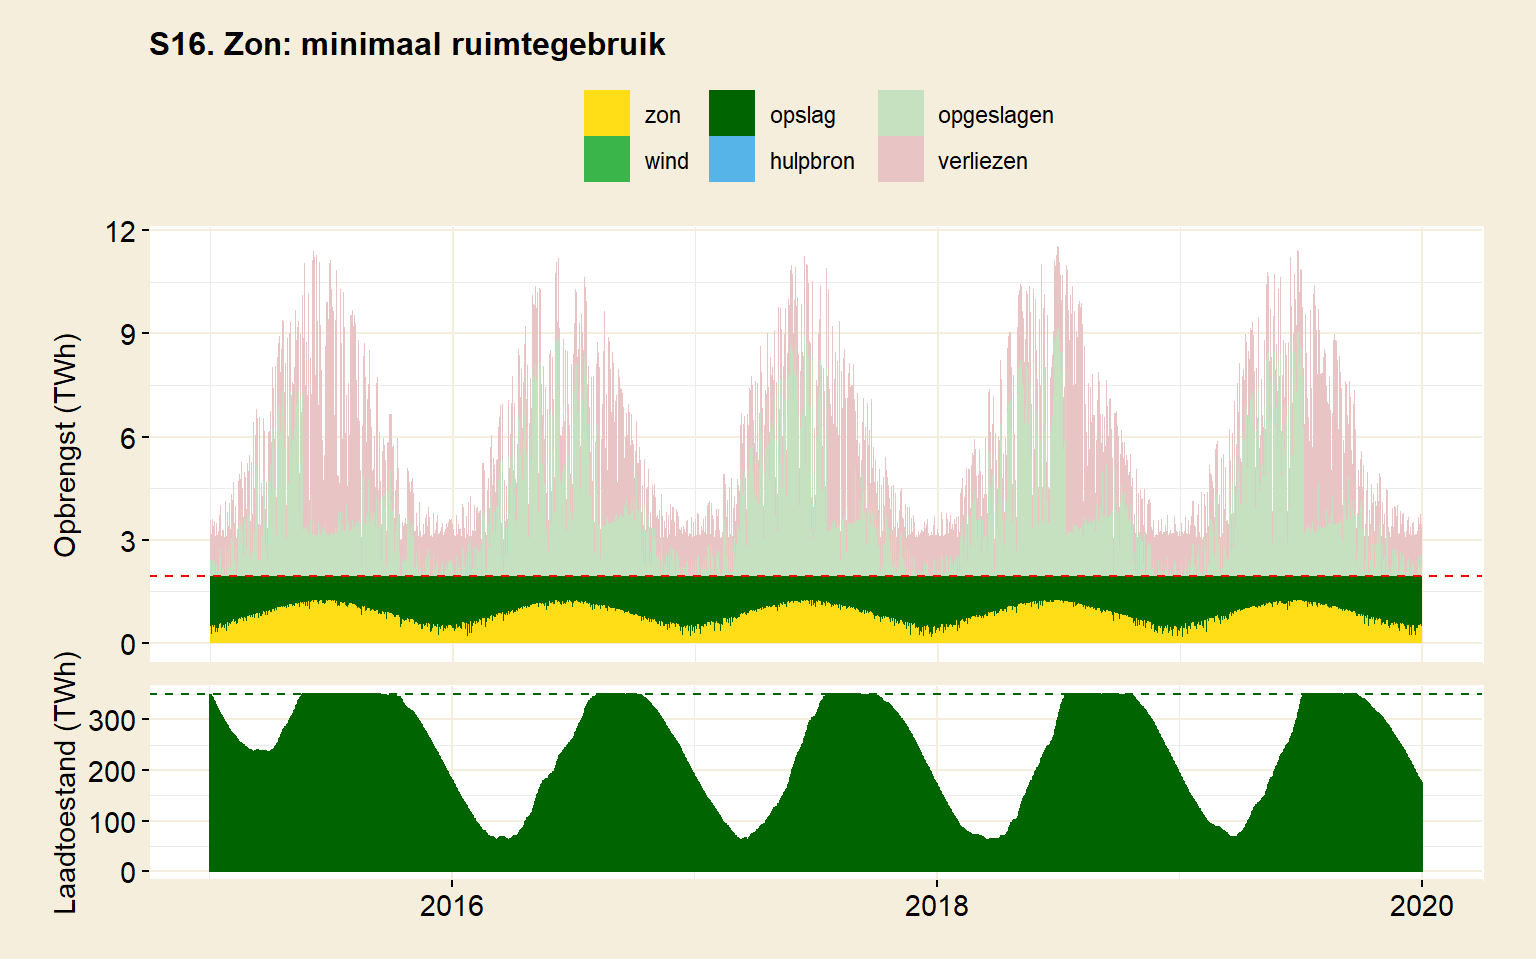
\includegraphics{06-Simulaties_files/figure-latex/unnamed-chunk-15-1} 

}

\end{figure}

In figuur S16 lukt dat. Er wordt geen gebruik gemaakt van een hulpbron. Desondanks kan er altijd aan de energievraag worden voldaan. Om dat te bereiken blijkt er 6000 km\textsuperscript{2} aan zonnecellen nodig. Dat is ook zo'n beetje het kantelpunt. Bij minder oppervlak moet de hulpbron al snel worden ingezet. Het model gebruikt 14\% van het landoppervlak voor zonnecellen. Dat komt neer op een kwart van de landbouwgrond (gebruik figuur 2.3 om uw eigen keuze te maken). Hier wordt overigens ook duidelijk dat plaatsing van zonnecellen op daken, waarbij de gebruikte ruimte niet onbruikbaar wordt, weinig zinvol is. Het benodigde oppervlak is daarvoor veel te groot.

De figuur laat zien dat de opslagcapaciteit voor deze periode voldoende is. De opslag raakt niet leeg. Ook een langere periode van 19 jaar liet zien dat de opgestelde infrastructuur voldoende zou zijn (niet getoond). De invloed der seizoenen komt in de opslag goed naar voren. Er is een mooie golfbeweging in de laadtoestand te zien. Omdat de opslag zo groot is, gaat er relatief weinig van de energieproductie verloren. Er is capaciteit genoeg om de overproductie van zonne-energie te kunnen opslaan.

Daarmee hebben we een schatting voor een minimum aan zonoppervlak. Die schatting is natuurlijk wel afhankelijk van hoe realistisch 350 TWh aan waterstofopslag in de toekomst zal blijken te zijn.

Er is nog een tweede belangrijk voorbehoud. Waar windenergie meer over het jaar verspreid is, piekt de opbrengst van zon nogal in de zomer. Dat leidt tot hoge vermogens. De opslag moet in staat zijn dat piekvermogen te kunnen verwerken. Het model schat de laadstroom in op maar liefst 9x het nationaal energieverbruik. Dat is een enorme laadstroom.

Hier toont zich de keerzijde van energie opwekken met zon. Een piekvermogen van 9 maal het Nederlands energieverbruik staat gelijk aan de simultane energieproductie van 490 Eemscentrales ('s lands grootste energiecentrale) op vol vermogen. Al dat vermogen moet per ommegaande kunnen worden omgezet in waterstof, gecomprimeerd, en onder de grond worden gestopt. Dat is nogal een taak. Het model zegt niets over hoe realistisch het is om dat op tijd te kunnen verwerken.

De omzetting naar waterstof vergt volgens het model 7500 waterstoffabrieken. Hoewel hier niet meegenomen, zal ook de infrastructuur voor compressie navenant moeten zijn. Krijg je zoveel waterstof snel genoeg onder de grond? Al met al stof om over na te denken, want het succes van deze opslagmethode hangt er van af.

\bigskip\noindent
De andere knop om aan te draaien, de hoeveelheid zonnecellen, blijkt minder zinvol te zijn. Vergelijk om dat te zien scenario S16 met S17 (tabel 5.6). Om de capaciteit van de opslag een orde van grootte naar beneden te krijgen (van 350 TWh naar 30 TWh), zou 85\% van Nederland beschikbaar moeten worden gesteld voor zonnecellen. Dat is niet haalbaar.

\bigskip

Tot slot dan: alleen de zon gebruiken voor onze energievoorziening, is dat een goed idee? Zoals eerder ook het geval was vergt dat vertrouwen in een oplossing die technisch nog ontwikkeld moet worden: massaopslag met behulp van waterstof. Een scenario dat zon combineert met opslag moet daarbij in staat zijn om te gaan met enorme laadstromen. Of dat kan? Wie het weet mag het zeggen. Deze grote laadstromen, in combinatie met het feit dat voor waterstofopslag zowiezo verschillende soorten infrastructuur naast elkaar nodig zijn, leidt tot een grote hoeveelheid infrastructuur. Dat zal zijn weerslag hebben op de betaalbaarheid van de oplossing.

\begin{table}

\caption{\label{tab:unnamed-chunk-16}Alleen zon}
\centering
\fontsize{9}{11}\selectfont
\begin{tabular}[t]{>{}l|>{\raggedleft\arraybackslash}p{2.5cm}>{\raggedleft\arraybackslash}p{2.5cm}>{\raggedleft\arraybackslash}p{2.5cm}}
\toprule
\em{\textbf{\em{}}} & \em{\textbf{S15. Alleen zon}} & \em{\textbf{S16. Zon, ruimte geminimaliseerd}} & \em{\textbf{S17. Zon, opslag geminimaliseerd}}\\
\addlinespace[0.3em]
\multicolumn{4}{l}{\textbf{Verbruik}}\\
\em{\hspace{1em}Jaarverbruik} & 706 TWh & 706 TWh & 706 TWh\\
\em{\hspace{1em}Aan waterstof} & 25 \% & 25 \% & 25 \%\\
\em{\hspace{1em}Aan elektriciteit} & 75 \% & 75 \% & 75 \%\\
\addlinespace[0.3em]
\multicolumn{4}{l}{\textbf{Ruimtegebruik}}\\
\em{\hspace{1em}Oppervlakte zon} & 8 \% NL & 14 \% NL & 85 \% NL\\
\em{\hspace{1em}Oppervlakte wind} & 0 \% NL & 0 \% NL & 0 \% NL\\
\addlinespace[0.3em]
\multicolumn{4}{l}{\textbf{Capaciteit}}\\
\em{\hspace{1em}Zon} & 100 \% & 190 \% & 1130 \%\\
\em{\hspace{1em}Wind} & 0 \% & 0 \% & 0 \vphantom{1} \%\\
\em{\hspace{1em}Hulpbron} & 100 \% & 0 \% & 0 \%\\
\em{\hspace{1em}Opslag} & 0 TWh & 350 TWh & 30 TWh\\
\addlinespace[0.3em]
\multicolumn{4}{l}{\textbf{Levering}}\\
\em{\hspace{1em}Zon} & 38 \% & 43 \% & 49 \%\\
\em{\hspace{1em}Wind} & 0 \% & 0 \% & 0 \%\\
\em{\hspace{1em}Hulpbron} & 62.2 \% & 0 \% & 0 \%\\
\em{\hspace{1em}Opslag} & 0 \% & 57 \% & 51 \%\\
\addlinespace[0.3em]
\multicolumn{4}{l}{\textbf{Verliezen}}\\
\em{\hspace{1em}Onbenut zon \& wind} & 60 \% & 28 \% & 967 \%\\
\em{\hspace{1em}Omzettingsverliezen} & 17 \% & 68 \% & 63 \%\\
\addlinespace[0.3em]
\multicolumn{4}{l}{\textbf{Draaitijd hulpbron}}\\
\em{\hspace{1em}Totale draaitijd} & 71.6 \% & 0 \% & 0 \%\\
\em{\hspace{1em}Draaitijd op > 90\% verm.} & 53.3 \% & 0 \% & 0 \%\\
\addlinespace[0.3em]
\multicolumn{4}{l}{\textbf{Laadvermogen opslag}}\\
\em{\hspace{1em}Maximaal} & 0 GW & 1396 GW & 3772 GW\\
\em{\hspace{1em}Gemiddelde top 20\%} & 0 GW & 737 GW & 1441 GW\\
\em{\hspace{1em}Max. ontladen elektr.} & 0 GW & 45 GW & 45 GW\\
\addlinespace[0.3em]
\multicolumn{4}{l}{\textbf{Inventaris}}\\
\em{\hspace{1em}Hulpcentrales (3 GW)} & 27 & 0 & 0\\
\em{\hspace{1em}Waterstoffabrieken (100 MW)} & 0 & 7366 & 14412\\
\em{\hspace{1em}Waterstofcentrales (3 GW)} & 0 & 20 & 20\\
\em{Periode} & 2015 - 2019 & 2015 - 2019 & 2015 - 2019\\
\bottomrule
\multicolumn{4}{l}{\rule{0pt}{1em}Voor een toelichting op de tabel, zie einde van dit hoofdstuk.}\\
\end{tabular}
\end{table}

\newpage

\hypertarget{helpt-besparen-bij-de-opvang-van-fluctuaties}{%
\subsection{Helpt besparen bij de opvang van fluctuaties?}\label{helpt-besparen-bij-de-opvang-van-fluctuaties}}

Besparen op het energieverbruik vermindert de uitstoot van CO\textsubscript{2}. Dat is directe winst in de transitieperiode, waar er nog gebruik wordt gemaakt van fossiele brandstof. Als de energieproductie echter eenmaal schoon is, wordt uit dat oogpunt besparing overbodig.

Een tweede reden om te bezuiningen, is om de energievraag te verkleinen. Er is dan minder infrastructuur nodig. Dat is vooral gunstig bij energieopwekking door bronnen met een lage energiedichtheid, zoals zon en wind. Er is dan minder schaarse ruimte nodig en het verminderd het probleem van fluctuaties. In het geval van kernenergie dient het niet echt een doel.

Als bezuinigen gebruikt wordt om de plaatsing van windmolens en zonnecellen beheersbaar te houden, dan krijgt de besparing een permanent karakter. Anders dan bijvoorbeeld de autoloze zondagen uit de jaren '70, destijds veroorzaakt door een olieboycot, gaat het niet om een tijdelijk tekort. Nederland blijft een klein grondgebied houden.

Daarmee loopt men het risico zichzelf in een hoekje te schilderen. Bij eerdere simulaties bleek dat wind en zon veel ruimte nodig hebben. Dat beperkt de mogelijkheid tot groei (extra energieverbruik bijv. voor verbetering van de gezondheidszorg, terugvangen van CO\textsubscript{2}, betere voedselproductie). Als bezuinigen wordt gebruikt als oplossing voor ruimtegebrek, dan zit men er aan vast.

\bigskip\noindent
Besparen zou een gunstig effect kunnen hebben op de hoeveelheid opslagcapaciteit die nodig is. Gebruikt men wind en zon, maar niet kernenergie, dan is opslag onontbeerlijk. De benodigde infrastructuur kan kleiner zijn als er bespaard wordt. Dat is een voordeel bij waterstofopslag, waarvoor de infrastructuur nogal omvangrijk zou zijn. Als de besparing groot genoeg is, kan uitval wellicht zelfs met lithiumaccu's worden opgevangen. Dat biedt voordeel omdat opslag in accu's minder complex is dan waterstofopslag.

In scenario 10 bleek dat er 150 TWh aan opslag nodig was om de energievoorziening op peil te houden. Dat geeft een startpositie om besparingen mee te vergelijken. Dat scenario gebruikte wind en zon, waarbij er overcapaciteit werd gecreëerd door het aantal zonnecellen te vergroten.

Scenario 18 voert verregaande bezuinigingen door en bespaart daarmee de helft op ons energieverbruik. Voor het overige blijft het scenario gelijk aan scenario 10. Zie tabel 5.7.

\begin{figure}

{\centering 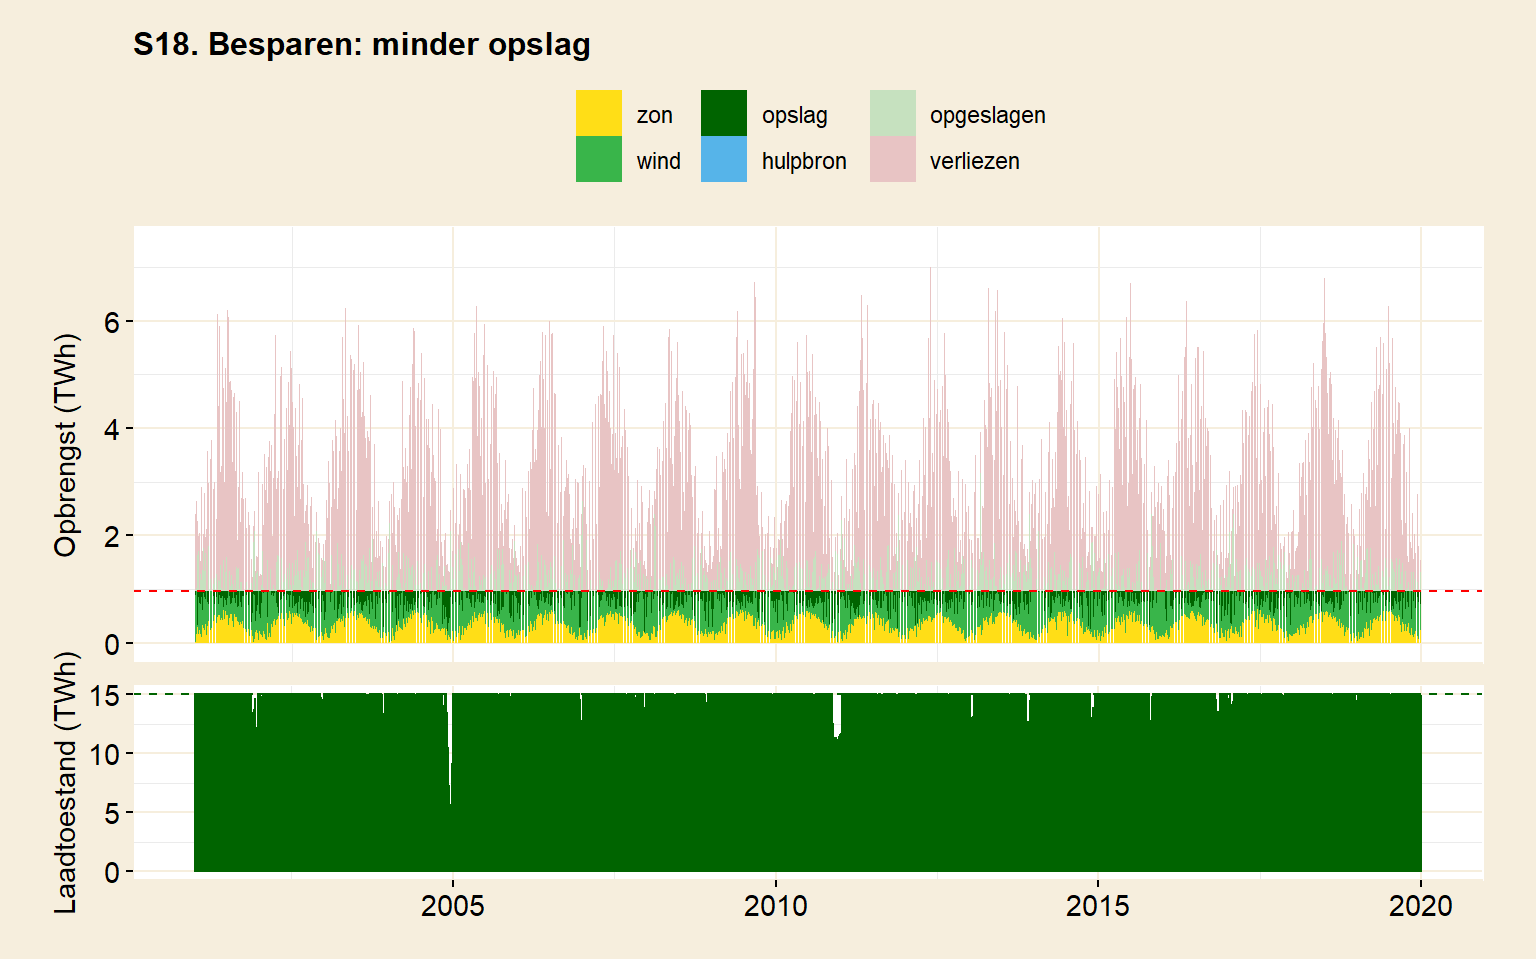
\includegraphics{06-Simulaties_files/figure-latex/unnamed-chunk-17-1} 

}

\end{figure}

Vijfig procent besparen is natuurlijk veel. Niet-energetisch gebruik werd al buiten beschouwing gelaten. Dat waren voornamelijk grondstoffen die aan de basis staan van producten. Op lange termijn zullen die natuurlijk wel vervangen moeten worden. Om toekomstbestendig te zijn, zouden die eigenlijk moeten worden meegerekend. De voorgestelde bezuiniging komt hier nogeens bovenop.

De simulatie laat zien dat besparen een groot effect heeft op de benodigde hoeveelheid opslag. Het halveren van het energiegebruik vermindert de opslagbehoefte met een factor tien. De opslag kan een orde van grootte kleiner. Wel is het effect van de bezuiningen volgens het model nog steeds onvoldoende om energieopslag in accu's plausibel te maken. Dat zou het gebruik van een elektrisch wagenpark zinvol maken, maar de benodigde capaciteit is daarvoor ruimschoots te groot.

\bigskip\noindent
Besparingen kunnen ook gebruikt worden om het areaal aan zonnecellen en windmolens te beperken. Kleiner ruimtegebruik heeft als voordeel dat de implementatie makkelijker wordt. Het vermindert bijvoorbeeld het overleg met belanghebbenden die medewerking moeten verlenen om molens of zonnecellen geplaatst te krijgen.

\begin{figure}

{\centering 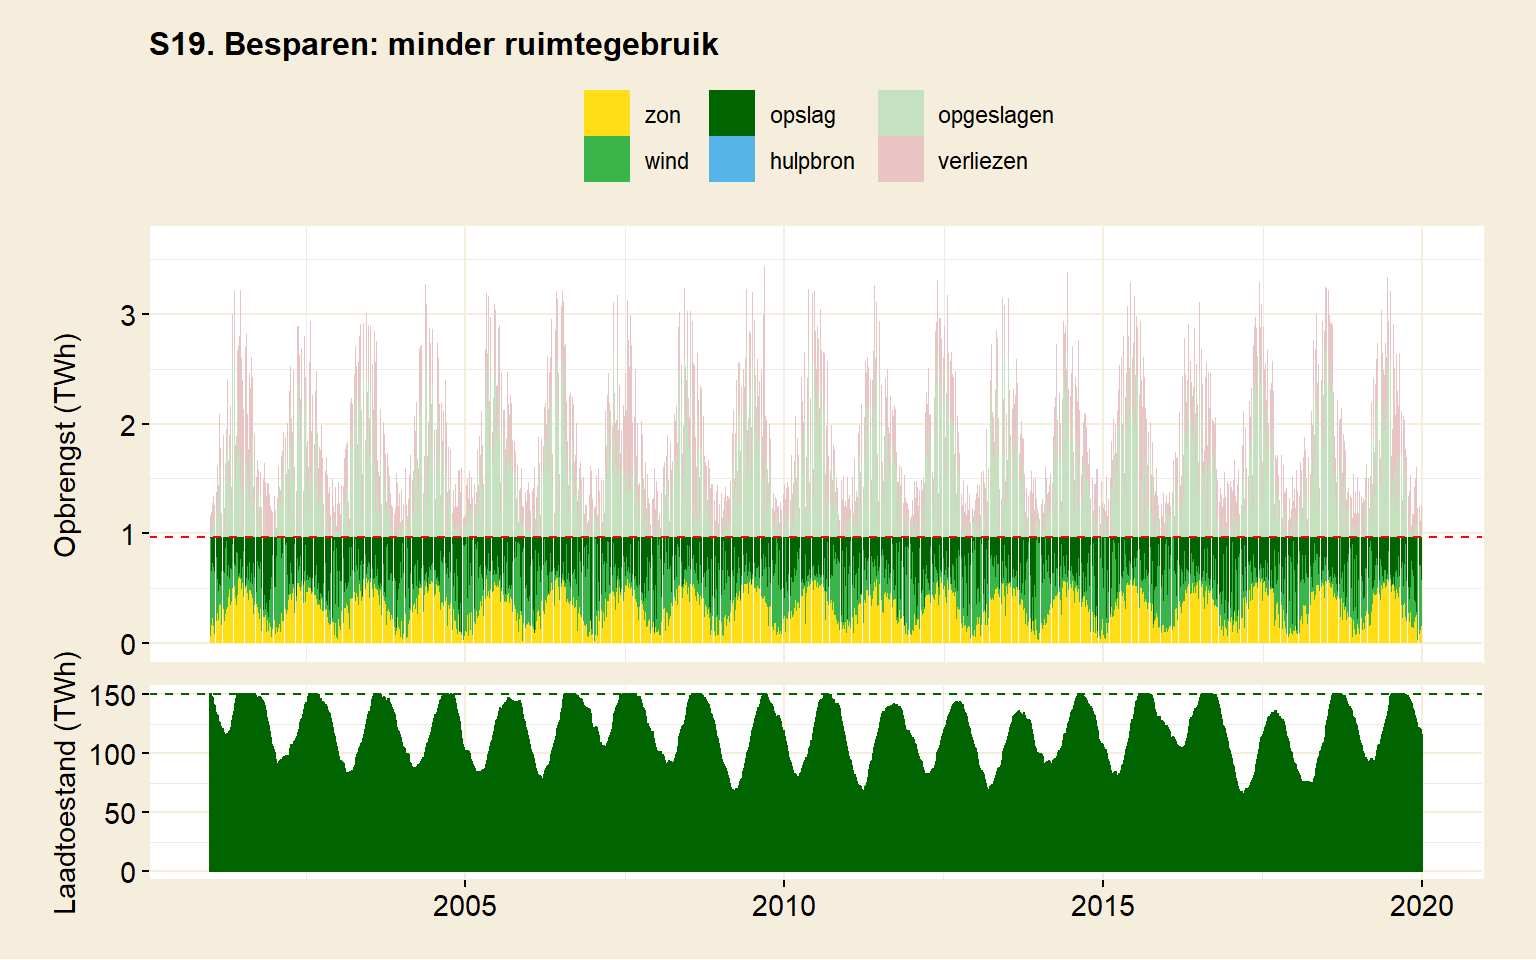
\includegraphics{06-Simulaties_files/figure-latex/unnamed-chunk-18-1} 

}

\end{figure}

Scenario 19 bezuinigt wederom 50\% op ons energieverbruik. Ditmaal blijft de hoeveelheid opslag constant ten opzichte van scenario 10. Nu gaat de hoeveelheid zonne- en windenergie worden gevarieerd.

\begin{table}

\caption{\label{tab:unnamed-chunk-19}Besparen}
\centering
\fontsize{9}{11}\selectfont
\begin{tabular}[t]{>{}l|>{\raggedleft\arraybackslash}p{2.5cm}>{\raggedleft\arraybackslash}p{2.5cm}>{\raggedleft\arraybackslash}p{2.5cm}>{\raggedleft\arraybackslash}p{2.5cm}}
\toprule
\em{\textbf{\em{}}} & \em{\textbf{S10. Waterstof lange termijn}} & \em{\textbf{S18. Besparen: minder opslag}} & \em{\textbf{S19. Besparen: minder ruimtegebruik}} & \em{\textbf{S20. Besparen: 25\% minder}}\\
\addlinespace[0.3em]
\multicolumn{5}{l}{\textbf{Verbruik}}\\
\em{\hspace{1em}Jaarverbruik} & 706 TWh & 353 TWh & 353 TWh & 530 TWh\\
\em{\hspace{1em}Aan waterstof} & 25 \% & 25 \% & 25 \% & 25 \%\\
\em{\hspace{1em}Aan elektriciteit} & 75 \% & 75 \% & 75 \% & 75 \%\\
\addlinespace[0.3em]
\multicolumn{5}{l}{\textbf{Ruimtegebruik}}\\
\em{\hspace{1em}Oppervlakte zon} & 8 \% NL & 8 \% NL & 4 \% NL & 8 \% NL\\
\em{\hspace{1em}Oppervlakte wind} & 52 \% NL & 52 \% NL & 21 \% NL & 52 \% NL\\
\addlinespace[0.3em]
\multicolumn{5}{l}{\textbf{Capaciteit}}\\
\em{\hspace{1em}Zon} & 100 \% & 200 \% & 100 \% & 133 \%\\
\em{\hspace{1em}Wind} & 50 \% & 101 \% & 40 \% & 67 \%\\
\em{\hspace{1em}Hulpbron} & 0 \% & 0 \% & 0 \% & 0 \vphantom{1} \%\\
\em{\hspace{1em}Opslag} & 150 TWh & 15 TWh & 150 TWh & 60 TWh\\
\addlinespace[0.3em]
\multicolumn{5}{l}{\textbf{Levering}}\\
\em{\hspace{1em}Zon} & 33 \% & 35 \% & 34 \% & 34 \%\\
\em{\hspace{1em}Wind} & 37 \% & 47 \% & 32 \% & 41 \%\\
\em{\hspace{1em}Hulpbron} & 0 \% & 0 \% & 0 \% & 0 \%\\
\em{\hspace{1em}Opslag} & 30 \% & 18 \% & 34 \% & 24 \%\\
\addlinespace[0.3em]
\multicolumn{5}{l}{\textbf{Verliezen}}\\
\em{\hspace{1em}Onbenut zon \& wind} & 17 \% & 178 \% & 4 \% & 72 \%\\
\em{\hspace{1em}Omzettingsverliezen} & 33 \% & 23 \% & 37 \% & 28 \%\\
\addlinespace[0.3em]
\multicolumn{5}{l}{\textbf{Draaitijd hulpbron}}\\
\em{\hspace{1em}Totale draaitijd} & 0 \% & 0 \% & 0 \% & 0 \%\\
\em{\hspace{1em}Draaitijd op > 90\% verm.} & 0 \% & 0 \% & 0 \% & 0 \%\\
\addlinespace[0.3em]
\multicolumn{5}{l}{\textbf{Laadvermogen opslag}}\\
\em{\hspace{1em}Maximaal} & 750 GW & 686 GW & 413 GW & 689 GW\\
\em{\hspace{1em}Gemiddelde top 20\%} & 330 GW & 193 GW & 183 GW & 247 GW\\
\em{\hspace{1em}Max. ontladen elektr.} & 45 GW & 22.5 GW & 22.5 GW & 33.75 GW\\
\addlinespace[0.3em]
\multicolumn{5}{l}{\textbf{Inventaris}}\\
\em{\hspace{1em}Hulpcentrales (3 GW)} & 0 & 0 & 0 & 0\\
\em{\hspace{1em}Waterstoffabrieken (100 MW)} & 3298 & 1931 & 1832 & 2472\\
\em{\hspace{1em}Waterstofcentrales (3 GW)} & 20 & 10 & 10 & 15\\
\em{Periode} & 2001 - 2019 & 2001 - 2019 & 2001 - 2019 & 2001 - 2019\\
\bottomrule
\multicolumn{5}{l}{\rule{0pt}{1em}Voor een toelichting op de tabel, zie einde van dit hoofdstuk.}\\
\end{tabular}
\end{table}

Het model kan in scenario 19 af met ongeveer de helft van de infrastructuur. De afname is lineair; lang niet zo groot als voor de opslagcapaciteit. Dat betekent dat besparen om oppervlakgebruik te verminderen wat minder zinvol is.

\bigskip\noindent
Tot slot is er in tabel 7 een scenario opgenomen waarin er iets minder drastisch wordt bespaard op ons energiegebruik. Scenario 20 simuleert een bezuiniging van 25\%. De benodigde opslagcapaciteit kan vervolgens meer dan gehalveerd worden. De effectiviteit van kleinere besparingen neemt dus snel af.

\newpage

\hypertarget{kan-beperkte-inzet-van-fossiele-brandstoffen-gebruikt-worden-om-fluctuaties-op-te-vangen-terwijl-we-wachten-op-innovatie}{%
\subsection{Kan beperkte inzet van fossiele brandstoffen gebruikt worden om fluctuaties op te vangen, terwijl we wachten op innovatie?}\label{kan-beperkte-inzet-van-fossiele-brandstoffen-gebruikt-worden-om-fluctuaties-op-te-vangen-terwijl-we-wachten-op-innovatie}}

Het opvangen van de fluctuaties in het aanbod van zonne- en windenergie door fossiele brandstofcentrales is interessant genoeg de situatie waarin Nederland zich nu bevindt. Het is duidelijk een overgangsscenario, tenminste als in de toekomst de energieproductie CO\textsubscript{2}-neutraal moet zijn. Maar misschien kan er worden gesmokkeld. Een beetje bijdraaien met fossiele brandstoffen is toch niet zo erg?

Groene energiebronnen worden op dit moment gebruikt om onze elektriciteitsbehoefte aan te vullen. In het hoofdstuk over verbruik werd duidelijk dat 8\% van onze energie `groen' wordt opgewekt. Het aandeel zon en wind komt niet verder dan 2,1\%. Het overige deel kwam van het verbanden van biomassa. Er werd geconcludeerd dat het verbranden van biomassa geen toekomstbestendig groeipad biedt. Biomassa heeft een extreem lage energiedichtheid. (Dat is de reden dat de simulaties alleen uitgaan van zon en wind.) Als zon en wind in de toekomst de oplossing gaan bieden, dan ligt er dus nog een stevig groeipad voor de boeg. De capaciteit moet vervijftigvoudigd worden.

Op dit moment kan er nog niet volhartig worden gekozen voor een scenario waar (waterstof)opslag gebruikt wordt om vraag en aanbod op elkaar te laten aansluiten. De techniek voor opslag op de schaal waarop we dat nodig hebben, is nog niet voor handen (zie hoofdstuk opslag, i.c.m. de simulaties). Dat betekent dat er gewacht moet worden op innovaties. In het gunstigste geval blijken die inderdaad haalbaar en komen nieuwe oplossingen `snel' beschikbaar. Er is ook een kans dat het langer duurt, en Nederland nog wel even vastzit aan fossiele brandstoffen. In de tussentijd moeten de fluctuaties veroorzaakt door een groeiend aandeel van zon en wind worden opgevangen, om uitval te voorkomen.

\bigskip\noindent
In het model worden fossiele brandstofcentrales gezien als hulpbron, net als kerncentrales. Aan een scenario met zon, wind en de beperkte inzet van kernenergie werd elders al gerekend. De resultaten zijn hier ook bruikbaar.

In een bezetting waarbij zon en wind in principe onze energiebehoefte zouden kunnen dekken, bleek een derde van de energiebehoefte toch uit centrales te komen (scenario 12). In scenario 13 werd uitgegaan van een extreme bezetting van windmolens en zonnecellen. Een kwart van Nederland werd gebruikt voor zonnecellen en anderhalf keer het oppervlak van Nederland voor windmolens. Hulpcentrales waren daar verantwoordelijk voor 13,5\% van de vraag.

Volgens het model is het dus niet makkelijk om de hoeveelheid uitstoot te beperken. Alleen door een extreme hoeveelheid ruimte op te offeren kan de uitstoot worden gedecimeerd.

De hoeveelheid uitstoot uit fossiele brandstofcentrales wordt dus bepaald door hoeveel energie er moet worden bijgedraaid. Daarnaast is er de vraag hoeveel centrales daarvoor dan nodig zijn. Zijn er daar al voldoende van?

Uit scenario's 12, 13 en 14 bleek dat kerncentrales 100\% van de nationale energievraag op de schouders moeten kunnen nemen. Hetzelfde zou gelden voor energiecentrales die op fossiele brandstoffen werken. Het vermogen van bestaande energiecentrales komt in totaal neer op 25\% van de Nederlandse energiebehoefte. Dat is op dit moment voldoende om het variabele deel van het aanbod (2,1\% van het energieverbruik) op te vangen. Als het vermogen in wind en zon groeit, zullen er fossiele brandstofcentrales moeten worden bijgebouwd. Dat zal het geval zijn als wind en zon meer dan 25\% van de energiebehoefte gaan leveren. Bij een voltooide energietransitie moeten er zelfs drie keer meer centrales worden bijgebouwd dan er nu staan.

Het moeten bijbouwen van centrales zou geen gunstige ontwikkeling zijn. Dat vormt een uitbreiding in fossiel, in plaats van een teruggang. Uiteindelijk zal men van de centrales afwillen. Wie wil er investeren in centrales die na voltooiing van de energietransitie weer moeten worden afgebroken? Dat geldt temeer als de energielevering uit deze centrales beperkt blijft (en dat is het doel). Er valt dan weinig te verdienen aan centrales die straks weer moeten worden afgebroken. Dat bemoeilijkt commerciële exploitatie.

\newpage
\scriptsize

\noindent

\hypertarget{tabeltoelichting}{%
\subsection{Tabeltoelichting}\label{tabeltoelichting}}

\bigskip

\noindent 
\textbf{Verbruik}. \emph{Jaarverbruik}: het totale energieverbruik in een gesimuleerd jaar. Indien meer dan een jaar wordt gesimuleerd is dit jaarverbruik het gemiddelde over de gehele periode. \emph{Aan waterstof}: aandeel van het totale verbruik dat wordt afgenomen in de vorm van waterstof. \emph{Aan elektriciteit}: idem, maar voor elektriciteit.

\noindent 
\textbf{Ruimtegebruik}. \emph{Oppervlakte zon}: het totale oppervlak aan zonnecellen waarvan de simulatie uitgaat. Zonnecellen zijn aaneensluitend geplaatst. \emph{Oppervlakte wind}: het totale oppervlak dat nodig is om windmolens te plaatsen, op basis van de gesimuleerd Enercon-126. De molens staan dan bijna 900m uit elkaar en zijn 200m hoog.

\noindent 
\textbf{Capaciteit}. \emph{Zon}: De hoeveelheid energie die in een jaar door zon kan worden opgewekt, tov het totaalverbruik. Voorbeeld: is de capaciteit 50\% en het jaarverbruik 706 TWh, dan wekt de zon in een jaar 353 TWh aan energie op. Niet alle energie die wordt geproduceerd, wordt echter ook daadwerkelijk geleverd en gebruikt. Er kan bijvoorbeld teveel aan zonne-energie zijn en het surplus kan verloren gaan. Deze post geeft dus de potentie van zonne-energie weer. Indien meer dan een jaar wordt gesimuleerd, wordt de gemiddelde jaarlijkse potentiële capaciteit over de gehele periode weergegeven. \emph{Wind}: idem. \emph{Hulpbron}: de totale potentiële hoeveelheid energie die de hulpbron over een jaar kan leveren. Als de capaciteit 100\% is, dan zou de hulpbron in potentie in een jaar 706 TWh (het jaarverbruik) hebben kunnen leveren, als deze bron continu zou worden gebruikt. Om een grotere capaciteit te kunnen leveren, zijn in de praktijk meer energiecentrales (hulpbronnen) nodig. \emph{Opslag}: De capaciteit, in TWh ditmaal, van de in de simulatie gebruikte opslag. Deel deze waarde door het jaarverbruik om een percentage te verkrijgen, zoals voor de overige posten werd gebruikt.

\noindent 
\textbf{Levering}. \emph{Zon}: De hoeveelheid energie in een jaar, ten opzichte van het totaalverbruik, die door zon \emph{direct} aan afnemers van energie werd geleverd. (Energie uit zon kan ook zijn opgeslagen, of verloren zijn gegaan.) Indien meer dan een jaar wordt gesimuleerd, geeft dit het jaargemiddelde aan. \emph{Wind}: idem. \emph{Hulpbron}: De hoeveelheid energie t.o.v. het totaalverbruik dat door de hulpbron in totaal in een jaar werd geleverd. \emph{Opslag}: De hoeveelheid energie t.o.v. het totaalverbruik dat door de opslag in totaal in een jaar werd geleverd.

\noindent 
\textbf{Verliezen}. \emph{Onbenut}: de hoeveelheid energie, geproduceerd door variabele bronnen (zon en wind) die \emph{niet} direct kon worden geleverd aan afnemers, òf kon worden opgeslagen. Dit gebeurt als de opslag vol zit, of er geen opslag wordt gebruikt. \emph{Omzettingsverliezen}: diverse verliezen die worden gemaakt in omzettingsprocessen. Voorbeeld: bij elektriciteitsproductie door verbanding van waterstof gaat 50\% van de potentiële energie in de waterstof verloren.

\noindent 
\textbf{Draaitijd hulpbron}. \emph{Totale draaitijd}: de totale tijd dat een hulpbron actief was. Dit geeft de tijd aan waar de hulpbron nodig was om bij te springen tijdens energietekorten. In deze post wordt niet gekeken naar het geleverde vermogen. \emph{Draaitijd op \textgreater{} 90\% verm.}: De totale draaitijd van de hulpbron om meer dan 90\% vermogen. Dit geeft een benadering voor `de hulpbron wordt gebruikt op vol vermogen'. Dit gebeurt typisch bij (vrijwel) compleet gebrek aan zon of wind.

\noindent 
\textbf{Laadvermogen}. \emph{Maximaal}: Het maximum laadvermogen dat de opslag te verwerken kreeg. Dit getal heeft zijn weerslag op de benodigde hoeveelheid infrastructuur die de opslag nodig heeft. \emph{Gemiddelde top 20\%}: Het gemiddelde laadvermogen van de top 20\% aan perioden van 10 minuten. Dit getal geeft een conservatieve schatting voor `maximaal laadvermogen opslag'. \emph{Max ontladen elektr.}: Dit is het maximale vermogen waarmee de opslag werd \emph{ont}laden. Dat heeft zijn weerslag op de hoeveelheid infrastructuur die nodig is. Voorbeeld: bij verbranding van waterstof om elektriciteit te maken in het geval van een waterstofopslag, bepaald dit de hoeveelheid waterstofcentrales die benodigd zijn.

\noindent 
\textbf{Inventaris}. \emph{Hulpcentrales}: Het aantal hulpcentrales van 3 GW dat in de simulatie nodig is. \emph{Waterstoffabrieken}: Het aantal waterstoffabrieken van 100 MW dat nodig is om het aanbod van elektriciteit in de simulatie om te zetten in waterstof. (Een waterstoffabriek van 100 MW is nu nog toekomstmuziek, de grootste ter wereld telt 20 MW.) \emph{Waterstofcentrales}: Het aantal waterstofverbrandingscentrales dat in de simulatie nodig is om waterstof uit de opslag om te zetten in elektriciteit.

\normalsize

\hypertarget{epiloog}{%
\chapter*{Epiloog}\label{epiloog}}
\addcontentsline{toc}{chapter}{Epiloog}

Nederland blijkt nog niet zo ver te zijn met schone energieopwekking. Het aandeel CO\textsubscript{2}-vrije productie is klein. Het grootste deel van wat er nu schoon wordt opgewekt, is gebaseerd op een brandstof die nauwelijks schaalbaar is: bos en gewas.

Daar verandering in brengen zal niet gemakkelijk zijn. Nederland is een klein land met een grote energiebehoefte. De ruimte om de energiebehoefte te verkleinen lijkt beperkt. Efficiëntieverbeteringen zijn eindig, zeker als waterstof in de toekomst een rol gaat spelen. Bezuiningingen anders dan efficiëntieverbeteringen leiden in feite tot welvaartsverlies, en dat zal niet voor iedereen welkom zijn.

De energiebronnen die werden overwogen om CO\textsubscript{2}-vrij energie te produceren waren windenergie, zonne-energie en kernenergie. Welke oplossingen voor een energiemix zijn er voorstelbaar op basis van deze energiebronnen? Tijd voor een rondje langs de velden.

Een optie is om de toekomstige energiemix enkel te baseren op kernenergie. Dat is een continue energiebron, waardoor een investering in capaciteit die gelijk is aan het Nederlands verbruik volstaat (100\%). Als Nederland in de toekomst naast elektriciteit ook waterstof nodig heeft, hetgeen waarschijnlijk is, zal er ook geïnvesteerd moeten worden in waterstoffabrieken. De investering daarin is proportioneel met het verbruik. Verbruikt Nederland in de toekomst bijvoorbeeld voor 25\% van haar energiebehoefte waterstof, dan is daar een evenredige capaciteit in waterstoffabrieken voor nodig. Dat zou in dit scenario een totaalinvestering in capaciteit vragen van 125\%.

Een energiemix gebaseerd op zon of wind heeft een aanzienlijk lagere energiedichtheid dan een gebaseerd op fossiele brandstoffen of kernenergie. Vooral windenergie op land kost ruimte: de helft van onze energie opwekken met behulp van de wind vergt de helft van het Nederlandse landoppervlak. Zonne-energie is wat dat betreft gunstiger, maar ook daar zal het vereiste landgebruik offers vragen. Zonnepanelen laten weinig ruimte voor ander gebruik. De behoefte aan ruimte van deze energievormen maakt het realiseren van overcapaciteit er niet makkelijker op.

Daarnaast leveren wind en zon slechts met tussenpozen energie. Om de continuïteit van de energievoorziening te waarborgen, is een alternatieve energiebron noodzakelijk.

Het alternatief kan bestaan uit een hulpbron (kernenergie of, zolang de transitie duurt, energiecentrales gebaseerd op fossiele brandstoffen). Een andere mogelijkheid is de periodieke energieoverschotten uit zon of wind op te slaan en in te zetten bij tekorten.

Het curieuze bij het gebruik van een hulpbron als achtervang van variabele bronnen, is dat een beperkte bezetting onhaalbaar blijkt. Een hulpbron is volgens het model altijd nodig op volle capaciteit. Dat wil zeggen: een capaciteit die gelijk is aan het totale verbruik (100\%). Dat verdubbelt op zijn minst de investering in capaciteit: er staat dan 100\% of meer aan zon en wind, plus 100\% voor de hulpbron. Gebruikt men als hulpbron kernenergie, dan zijn zon en wind in feite overbodig. Fossiele brandstoffen zouden alleen een plaats hebben tijdens de transitie zelf, maar daar kleeft een nadeel aan. Naarmate wind en zon meer van onze energieproductie gaan overnemen, zullen er op een gegeven moment fossiele brandstofcentrales moeten worden bijgebouwd. Dat lijkt een beetje het paard achter de wagen spannen.

De combinatie van zonne- en windenergie met een hulpbron lijkt dus niet zo'n logische keuze. De andere optie die resteert is energieopslag. Opslag in accu's en spaarbekkens is gelimiteerd in capaciteit. Gebrek aan grondstoffen beperkt het gebruik van accu's, waar geografie de beperkende factor is voor spaarbekkens.

Dat capaciteitsprobleem kent waterstofopslag niet, althans niet in de Nederlandse context. Er zijn wel andere problemen.

Een energiemix gebaseerd op zonne- en windenergie en waterstofopslag liep volgens het model behoorlijk in de papieren. Dat kwam allereerst doordat er overcapaciteit in wind en zon nodig was. Daarnaast is er veel infrastructuur nodig om afdoende waterstofopslag te realiseren. Omdat waterstof gebruikt wordt als elektriciteitsbuffer, zijn er tevens energiecentrales nodig die waterstof in elektriciteit kunnen omzetten. Het model kwam in dit scenario op een investering in capaciteit van bijna 700\%. Het lijkt aannemelijk dat dit niet zonder gevolgen voor de energieprijs zal blijven. Men zal in dat geval bereid moeten zijn deze grotere complexiteit en kosten voor lief te nemen.

Er is nog een ander voorbehoud dat in dit scenario geaccepteerd zal moeten worden. Anders dan windmolens, zonnecellen, lithiumaccu's en kerncentrales is massa-opslag op basis van waterstof deels nog toekomstmuziek. Hoewel er geen fundamentele beperkingen lijken te zijn, moet de techniek nog op schaal worden ontwikkeld. Uieindelijk is er een grote hoeveelheid infrastructuur nodig. De vraag is daarmee hoe lang het gaat duren voordat een eventuele oplossing realiteit is. Daarmee blijft dit scenario risicovol.

\hypertarget{appendix-appendix}{%
\appendix}


\hypertarget{windenergie-1}{%
\chapter{Windenergie}\label{windenergie-1}}

\hypertarget{een-volmaakte-windmolen}{%
\section{Een volmaakte windmolen}\label{een-volmaakte-windmolen}}

\bigskip

Een enkele, `volmaakte' windmolen haalt het theoretisch maximum aan energie uit de langsstromende lucht. De hoeveelheid bewegingsenergie die lucht bevat is afhankelijk van de windsnelheid \(v\) en de luchtdichtheid \(\rho\) (1,3 kg/m\textsuperscript{3}). Bewegende lucht die stroomt door een vierkante meter heeft een vermogen dat gelijk is aan

\[ \frac{1}{2} \rho v^3 \]
\noindent
Watt (zie bijvoorbeeld \href{https://www.withouthotair.com/download.html}{MacKay}). Een windmolen met grotere wieken vangt meer wind en zal daardoor meer vermogen leveren. De oppervlakte die de wieken beslaan, een cirkel met een diameter \(d\), is gelijk aan \(\pi (\frac{1}{2} d)^2\). De stromende lucht door het oppervlak van de wieken kan dus een maximaal vermogen leveren van

\[ \frac{1}{2} \rho v^3 \times \pi  (\frac{1}{2} d)^2 = \frac{1}{2} \rho v^3 \; \frac{\pi}{4} d^2\]
\noindent
Watt. De molen zelf onttrekt energie aan de bewegende lucht en de lucht vertraagt daarmee. Zou je alle energie uit de lucht halen, dan waait het niet meer. En als het niet waait dan draait de molen niet meer. Er zit dus een maximum aan de hoeveelheid energie die men uit stromende lucht kan onttrekken.

\medskip

Een ander effect van de luchtvertraging is dat je windmolens niet te dicht bij elkaar kunt zetten. Ze hebben dan teveel last van elkaars windschaduw. Windparken houden doorgaans een afstand aan van tussen de \href{https://en.wikipedia.org/wiki/Wind_turbine\#Wind_turbine_spacing}{6-10 wiekdiameters}. Een windmolen bezet een landoppervlakte van \((sd)^2\) m\textsuperscript{2}, waarbij \(s\) de separatieafstand in wiekdiameters is. Als we ons nu afvragen hoeveel vermogen er door een windmolen per m\textsuperscript{2} landoppervlak kan worden gegenereerd, dan blijkt de diameter van de wieken weg te vallen (zie ook \href{https://www.withouthotair.com/download.html}{MacKay}):

\[ \frac{\frac{1}{2} \rho v^3 \frac{\pi}{4} d^2}{(sd)^2} = \; \frac{\pi}{8s^2} \; \rho v^3 \]
\noindent
De spanwijdte maakt dus niet uit! Grotere windmolens leveren meer vermogen, maar ze moeten ook verder uit elkaar geplaatst worden dan kleine molens. Het geleverde vermogen per vierkante meter is slechts afhankelijk van de windsnelheid en hoe ver de molens uit elkaar geplaatst worden.

\medskip

Een windmolen kan niet alle beschikbare kinetische energie die in wind zit onttrekken. Volgens de \href{https://nl.wikipedia.org/wiki/Wet_van_Betz}{wet van Betz} kan maximaal 59\% van deze energie worden omgezet. Een betere efficiëntie is niet haalbaar, hoe goed de windmolen ook ontworpen wordt. Een volmaakte molen heeft daarmee een opbrengst van

\[  59\% \times \frac{\pi}{8s^2} \; 1.3 v^3\approx \frac{0.3\;v^3}{s^2} \;  \]
Watt per m\textsuperscript{2}. We kunnen dus onafhankelijk van de grootte van de windmolen zeggen welke opbrengst we mogen verwachten als we uitgaan van een volmaakte windmolen.

\bigskip

Tot nu toe geeft de afgeleide formule de theoretische energie-opbrengst weer van een vierkante meter in een windmolenpark. Windmolens hebben echter last van elkaars windschaduw en met deze verliezen werd nog niet rekening gehouden. Hoe groot zijn deze verliezen?

\medskip

Uit onderzoek van \href{https://www.researchgate.net/publication/230284417_Optimal_turbine_spacing_in_fully_developed_wind_farm_boundary_layers}{Meyers \& Meneveau} blijkt dat windmolens die in een windpark zijn opgesteld veel turbulentie veroorzaken. Deze turbulentie zorgt voor een aanzienlijke vermindering van de opbrengst. Dit zorgt er voor dat de energie-opbrengst van een molen in een windpark minder is dan die van een alleenstaande molen.

\medskip

De figuur hieronder, overgenomen uit \href{https://www.researchgate.net/publication/230284417_Optimal_turbine_spacing_in_fully_developed_wind_farm_boundary_layers}{Meyers \& Meneveau}, toont het verband tussen efficiëntie en afstand. De figuur geeft vermogen van een molen staande in een oneindig windpark weer, ten opzichte van het vermogen van een alleenstaande molen. Het genormaliseerde vermogen is afgezet tegen de onderlinge afstand \(s\) in wiekdiameters.

\begin{figure}[H]

{\centering \includegraphics[width=0.35\linewidth,height=0.35\textheight]{D:/Dropbox/Maas/klimaat/klimaatR/VermogenVersusSeparatieafstandMolens} 

}

\caption{Efficiëntie ten opzichte van separatie-afstand}\label{fig:unnamed-chunk-1}
\end{figure}

\medskip

De theoretische benadering van \href{https://www.researchgate.net/publication/230284417_Optimal_turbine_spacing_in_fully_developed_wind_farm_boundary_layers}{Meyers \& Meneveau} wordt bevestigd door metingen aan windparken in de praktijk. De driehoeken in de figuur geven metingen weer van Horns Rev, een windpark op zee in Denemarken (\(s=7\)). Horns Rev haalt een efficiëntie van 60\% ten opzichte van een alleenstaande molen (\(P_\infty=0.6P\)). Pas bij een afstand van 100 maal de wiekdiameter nadert de efficiëntie de 100\%. Het onderzoek pleit voor een afstand van minimaal 15; volgens de grafiek is de efficiëntie dan zo rond de 80\%. Dat is een afstand die windparken in de praktijk op dit moment bij lange na niet hanteren.

\medskip

Dit verlies aan opbrengst moet worden verrekend. Het opwekken van grote hoeveelheden windenergie vereist de plaatsing van molens in windparken. De formule wordt daarom uitgebreid. De energie-opbrengst wordt vermenigvuldigd met de verwachte efficiëntie \(e_s\) van een windpark met molens:

\[  e_s \; \frac{0.3\;v^3}{s^2}  \]
De efficiëntie van een windmolenpark wordt dan aan de hand van de gekozen separatieafstand opgezocht in de figuur van Meyers \& Meneveau.

\hypertarget{windmolens-in-de-praktijk}{%
\section{Windmolens in de praktijk}\label{windmolens-in-de-praktijk}}

\bigskip

Een \href{https://en.wikipedia.org/wiki/Wind_turbine}{windmolen} wordt \href{https://en.wikipedia.org/wiki/Wind_turbine_design}{ontworpen} op het snelheidsbereik waarvan men de hoogste opbrengst verwacht. Buiten dat bereik is deze minder efficiënt. De onderstaande figuur geeft de vermogenscurve weer voor de Enercon-126, in magenta, zoals deze door de fabrikant wordt verstrekt. Tevens is de theoretische vermogenscurve weergegeven, in blauw, zodat beide met elkaar vergeleken kunnen worden. Een aantal dingen vallen op.

\medskip

De opbrengst van de Enercon ligt altijd lager dan de theoretische. Dat is natuurlijk de verwachting, want meer dan het theoretisch maximum kan men niet halen. De aard van beide curven is anders: waar het vermogen in theorie blijft stijgen bij toenemende windsnelheid, wordt de curve van een echte windmolen op een goed moment afgekapt. De Enercon komt tot een windsnelheid van 10 m/s goed mee met de theorie. Dit is het snelheidsbereik waarop de molen effectief is. Als men leest over de efficiëntie van windmolens - die halen tegenwoordig 80\% - dan is dat over dit snelheidsbereik. Boven de 15 m/s neemt het vermogen niet meer toe, en tussen de 25 en 35 m/s wordt de molen uitgeschakeld. Hier levert de molen bij lange na niet wat theoretisch verwacht zou worden.

\medskip

In de figuur naast de vermogenscurven bevindt zich een frequentiediagram van de windsnelheid. Het geeft aan hoe vaak een bepaalde windsnelheid voorkomt. Te zien is dat winsnelheden boven de 10 m/s relatief zeldzaam zijn. Het is waarschijnlijk geen toeval dat Enercon-126 ontworpen is effectief te zijn tot zo'n 10 m/s.

\medskip

Via numerieke integratie, de aanpak die hier wordt gebruikt, is te benaderen wat de opbrengstverschillen zijn. Telt men de opbrengsten over een langere periode (10 jaar) op, dan brengt de Enercon-126 in Nederland ongeveer de helft op van wat men theoretisch zou verwachten. Er is dus een groot verschil in opbrengst tussen theorie en praktijk. Met het huidige ontwerp van windmolens, die worden ontworpen op een bepaald snelheidsbereik, is niet te verwachten dat deze de theorie in de toekomst gaan benaderen.

\bigskip

\begin{center}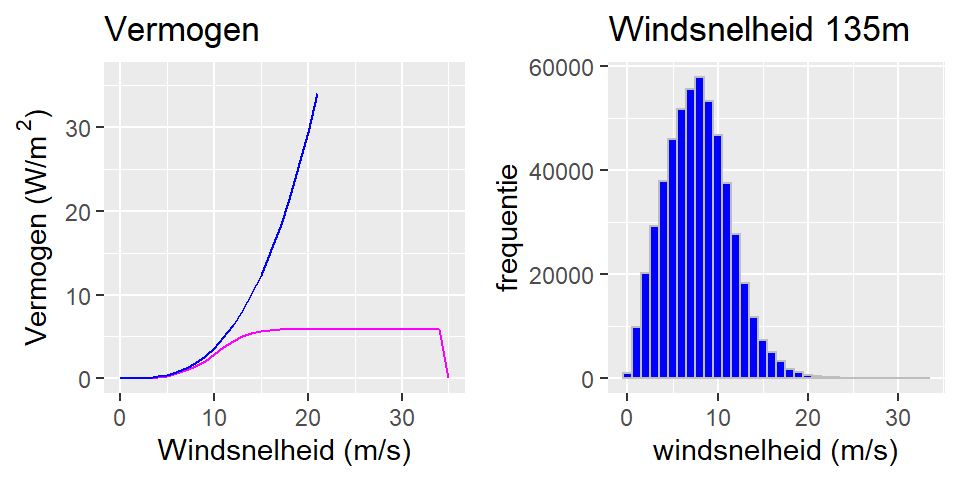
\includegraphics{08-Appendix_files/figure-latex/EnerconPowerCurve-1} \end{center}

\hypertarget{berekenen-van-opbrengst}{%
\section{Berekenen van opbrengst}\label{berekenen-van-opbrengst}}

\bigskip

Mocht dat in de toekomst wel lukken, dan geldt er echter een \emph{trade-off}. Als een windmolen het theoretisch maximum nadert, dan kan de molen per definitie beter gebruik maken van windvlagen, van hogere windsnelheden. Dat betekent ook dat daarmee de energie-opbrengst meer fluctueert. Deze fluctuaties zal men moeten opvangen. Het omgekeerde geldt ook: als een windmolen minder efficient is en minder goed energie kan halen uit hogere windsnelheden, dan zijn de fluctuaties minder. Dat gaat echter ten koste van de opbrengst en dat betekent dat men meer ruimte nodig heeft om molens te plaatsen.

\medskip

De bedoeling is hier om een realistische benadering te geven van de energie-opbrengst van een vierkante kilometer bezet met windmolens. Er worden hier twee benaderingen uitgewerkt: een theoretische en een praktische.

\medskip

Voor de theoretische benadering kan men uitgaan van de gemiddelde windsnelheid over een lange periode (zeg 10 jaar). Vervolgens kan deze worden gebruikt in de afgeleidde formule (\(P = e_s \; \frac{0.3\;v^3}{s^2}\)). Dat is de benadering die bijvoorbeeld \href{https://www.withouthotair.com/download.html}{MacKay} heeft gekozen. Voor een realistische schatting van energie-opbrengst heeft dat echter serieuze nadelen.

Volgens de formule verhoudt de opbrengst zich met de windsnelheid tot de derde macht. Het probleem met windsnelheid middelen over een langere periode is dat de opbrengst wordt onderschat. De gemiddelde windsnelheid in een maand tot de derde macht is kleiner dan de som van de dagelijkse windsnelheden tot de derde macht. Voorbeeld met twee winddagen: \(\frac{v_1^3 + v_2^3}{2} \neq (\frac{v_1+v_2}{2})^3\). Neem \(v_1=1\) en \(v_2=3\), dan volgt \(14 \neq 8\). Hoe korter de tijdsperiode is die wordt gehanteerd, hoe groter het uiteindelijke verschil is.

\medskip

Eenzelfde probleem geldt voor de praktijkbenadering waarbij wordt uitgegaan van de Enercon-126. De opbrengst wordt nu niet bepaald door een theoretische formule, maar door de windsnelheid op te zoeken in de vermogenscurve (power curve) zoals die wordt verstrekt door de leverancier van de molen. Zie ook bijlage A.2 \emph{windmolens in de praktijk}. Deze power curve heeft geen lineair verloop. Ook hier leidt het optellen van de opbrengst bij diverse windsnelheden tot een andere uitkomst dan het opzoeken van de opbrengst bij de gemiddelde windsnelheid.

\medskip

Om te komen tot een betere schatting van energie-opbrengst, wordt de opbrengst niet berekend aan de hand van de gemiddelde windsnelheid over de gehele periode, maar door tijdsvakken van 10 minuten te gebruiken. Het KNMI heeft \href{https://dataplatform.knmi.nl/dataset/cesar-tower-meteo-lc1-t10-v1-0}{data} beschikbaar die de windsnelheid iedere 10 minuten weergeeft op verschillende plaatsen en hoogten in Nederland. Aan de hand van deze data wordt voor ieder tijdsvak van 10 minuten de energie-opbrengst berekend.

\begin{table}[H]

\caption{\label{tab:datavoorbeeld1}Voorbeeld van opbrengstgegevens}
\centering
\fontsize{10}{12}\selectfont
\begin{tabular}[t]{r>{\raggedleft\arraybackslash}p{2cm}>{\raggedleft\arraybackslash}p{2cm}>{\raggedleft\arraybackslash}p{2cm}>{\raggedleft\arraybackslash}p{2cm}>{\raggedleft\arraybackslash}p{2cm}}
\toprule
Tijd & Wind (m/s) & Betz (W/m2) & Enercon-126 (W/m2) & Opbrengst Betz (kWh/km2) & Opbrengst Enercon-126 (kWh/km2)\\
\midrule
2007-04-01 00:00:00 & 12.4 & 7.00 & 4.67 & 1167.32 & 777.71\\
2007-04-01 00:10:00 & 11.7 & 5.88 & 4.23 & 980.58 & 704.44\\
2007-04-01 00:20:00 & 10.9 & 4.76 & 3.66 & 792.87 & 609.31\\
2007-04-01 00:30:00 & 10.8 & 4.63 & 3.57 & 771.25 & 595.17\\
2007-04-01 00:40:00 & 10.8 & 4.63 & 3.57 & 771.25 & 595.17\\
\bottomrule
\end{tabular}
\end{table}

\bigskip

Voor langere perioden wordt de opbrengst gesommeerd, bijvoorbeeld de dagopbrengst is gelijk aan de som van de 144 vakken van 10 minuten in die dag. De opbrengst wordt zowel berekend door gebruik te maken van de formule (hier `Betz' genoemd), als door de windsnelheid van iedere 10 minuten op te zoeken in de power curve van de Enercon-126. In tabel 1 is dat gedaan en ziet men enige uitkomsten zoals deze in de berekeningen zijn gebruikt.

\medskip

De theoretische opbrengst in W/m\textsuperscript{2}, de derde kolom (`Betz'), wordt berekend door de windsnelheid in de tweede kolom te nemen en in te vullen in \(e_s \; \frac{0.3\;v^3}{s^2}\) in \(v\) en voor \(s=7\) en \(e_s=0.6\) te nemen. De energie-opbrengst wordt berekend door W/m\textsuperscript{2} om te zetten in kWh per km\textsuperscript{2}. Voor de Enercon wordt in de power curve (zie bijlage A.2 \emph{windmolens in de praktijk}) de opbrengst in kW bij een bepaalde windsnelheid opgezocht. Dan wordt berekend wat er in kWh wordt geproduceerd op een oppervlak bezet met molens met een separatieafstand van 7 wiekdiameters. De laatste twee kolommen geven die opbrengst in kWh per vierkante kilometer weer voor `Betz' en de Enercon.

\bigskip

\begin{center}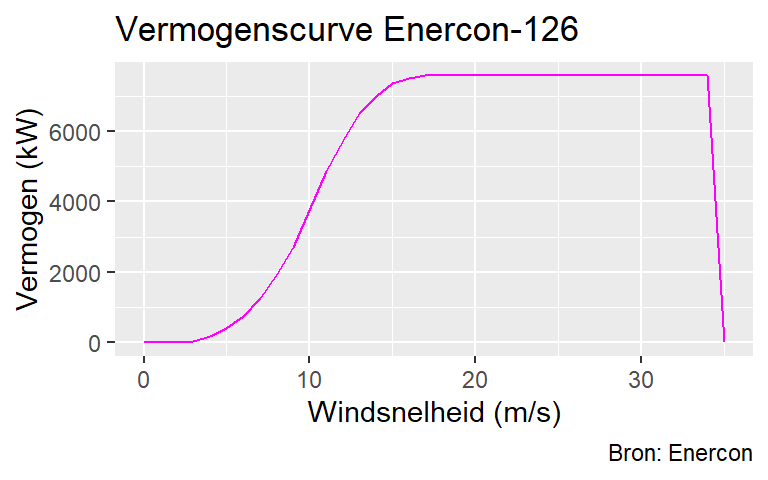
\includegraphics{08-Appendix_files/figure-latex/EnerconPowerCurve2-1} \end{center}

\hypertarget{berekenen-van-lopend-tekort}{%
\section{Berekenen van lopend tekort}\label{berekenen-van-lopend-tekort}}

\bigskip

Figuur 4 (zie tekst) geeft de maandelijkse tekorten en overschotten weer voor een windpark ten opzichte van de gemiddelde opbrengst van dat jaar. Het blijkt echter dat er grote maandelijkse verschillen zitten in de windkracht. Er zijn maanden met een overproductie t.o.v. het gemiddelde, en er zijn maanden met een tekort.

\medskip

Uit figuur 4 blijkt dat in 2007 de maand januari de meeste wind had. In deze maand zou 16,2\% van de jaaropbrengst zijn binnengekomen. De zomer daarentegen kent een periode van drie maanden achtereen met tekorten.

\medskip

In opeenvolgende maanden met tekorten stapelt het tekort zich vervolgens op, omdat de tekorten blijven aanhouden. Laten we eens kijken hoe dat in 2007 uitpakt. In 2007 was er van januari tot en met maart ruim voldoende wind voorhanden om aan de vraag te voldoen. Oktober daarentegen had een groot tekort. In die maand was er een tekort van 8,3\% - 4,6\% = 3,7\% van de jaarlijkse energiebehoefte. Dat is dus een tekort van 45\% (3,7 / 8,3 = 0,45) op maandbasis. Dat (lopende) tekort wordt de maand daarop in mei niet teruggewonnen, ondanks dat het een windrijke maand was. In juni, de maand daarna, verdiept het tekort verder. In totaal ontstaat er in 2007 zo een tekort dat oploopt tot (8,3-5,6) + (8,3-7,5) + (8,3-4,7) + (8,3-7,2) + (8,3-5,4) + (8,3-6,9) + (8,3-4,6) = 16,5\% van de opbrengst in dat jaar.

\medskip

In dit voorbeeld werden tekorten berekend aan de hand van maandopbrengsten. Een jaar heeft slechts 12 maanden, dus het blijft overzichtelijk en er valt gemakkelijk uit de grafiek te tellen. Het is wel een enigzinds grove telling zo. Naarmate het tijdsinterval afneemt zal het gemeten tekort toenemen. Immers, een maand die gemiddeld genoeg opbrengst heeft, kan best zijn begonnen met twee weken windstilte. Die windstilte blijft onzichtbaar, maar had eigenlijk bij een eventueel lopend tekort van vorige maanden moeten worden opgeteld. Om een betere benadering van het maximale tekort te krijgen worden de energietekorten elders in de tekst in tijdsvakken van 10 minuten berekend.

\hypertarget{zonne-energie-1}{%
\chapter{Zonne-energie}\label{zonne-energie-1}}

\hypertarget{berekenen-van-opbrengst-1}{%
\section{Berekenen van opbrengst}\label{berekenen-van-opbrengst-1}}

\medskip

Om de opbrengst van zonnecellen te berekenen wordt stralingsdata van het KNMI gebruikt, gemeten nabij meetmast Cabauw, midden in het land. De data geeft voor het tijdsvak van 10 minuten de gemiddelde globale straling in Watt per vierkante meter. Aan de hand van deze data wordt voor ieder tijdsvak van 10 minuten de energie-opbrengst berekend. Voor langere perioden wordt de opbrengst gesommeerd, bijvoorbeeld de dagopbrengst is gelijk aan de som van de 144 vakken van 10 minuten in die dag. In tabel B.1 ziet men enige uitkomsten zoals deze in de berekeningen zijn gebruikt.

\begin{table}[H]

\caption{\label{tab:datavoorbeeld2}Voorbeeld van opbrengstgegevens}
\centering
\fontsize{10}{12}\selectfont
\begin{tabular}[t]{r>{\raggedleft\arraybackslash}p{2cm}>{\raggedleft\arraybackslash}p{2cm}}
\toprule
Tijd & straling (W/m2) & Opbrengst zonnecel (kWh/km2)\\
\midrule
2007-04-01 09:50:00 & 575.48 & 19182.72\\
2007-04-01 10:00:00 & 589.89 & 19662.86\\
2007-04-01 10:10:00 & 597.83 & 19927.65\\
2007-04-01 10:20:00 & 608.60 & 20286.79\\
2007-04-01 10:30:00 & 620.90 & 20696.61\\
2007-04-01 10:40:00 & 630.46 & 21015.29\\
\bottomrule
\end{tabular}
\end{table}

\bigskip

In de tekst wordt uitgegaan van zonnepanelen met een rendement van 20\%. De opbrengst wordt weergegeven in kilowattuur per vierkante kilometer. De straling wordt door het KNMI in tijdsvakken van 10 minuten weergegeven in watt per vierkante meter (W/m\textsuperscript{2}). De berekeningen werken verder met de kilowattuur (kWh), dus de waarde in watt voor de 10 minuten wordt eerst omgezet naar wattuur. Daartoe wordt de waarde van de kolom straling gedeeld door 6: 575,48 W / 6 = 95,91 Wh (per 10 min). Vervolgens wordt er gedeeld door 1.000 om van W naar kW te komen en dan maal een miljoen om van vierkante meter naar vierkante kilometer te komen: (95,5 / 1.000) * 1.000.000 = 95.913,33 kWh/km\textsuperscript{2}. Dan, omdat de panelen een efficiëntie van 20\% hebben, blijft daar een vijfde van over. Daarmee wordt de uitkomst in de kolom `opbrengst' verkregen: 95.913,33 * 20\% = 19.182,72 kWh/km\textsuperscript{2}.

\end{document}
